\documentclass[12pt,a4paper,twoside,openright]{memoir}
%\usepackage[a4paper,width=140mm,top=35mm,bottom=35mm,bindingoffset=10mm]{geometry}
% Font encoding
\usepackage[T1]{fontenc}
% input encoding
\usepackage[utf8]{inputenc}
% Font package
\usepackage{kpfonts}
% Language package
\usepackage[english]{babel}
% Enhanced support for graphics
\usepackage{graphicx}
% Color addition
\usepackage[dvipsnames]{xcolor}
% Figure adding
\usepackage{subfig}
\usepackage{amsmath}
\newcommand{\norm}[1]{\left\lVert#1\right\rVert}
\usepackage{enumitem}
\usepackage{amsfonts}
\usepackage{amssymb}
\usepackage{amsthm}
\usepackage{amstext}
\newtheorem{theorem}{Theorem}[section]
\newtheorem{prop}{Proposition}[section]
\theoremstyle{definition}
\newtheorem{definition}{Definition}[section]
% Context sensitive quotation
\usepackage{csquotes}
% Algorithm package
\usepackage{algpseudocode}
\usepackage[section]{algorithm}

% Alias counters
%\usepackage{aliascnt}
% Bolding
\usepackage{bm}
% Environment package
\usepackage{verbatim}
% Multirow table
\usepackage{multirow}
% Line spacing
\usepackage{enumitem}
\setlist{nolistsep}
% Customize captions
\usepackage{caption}
\captionsetup[table]{labelfont={small,sc},font={small,sc},
labelsep=newline, justification=centering, skip=5pt, position=top}
\captionsetup[figure]{margin=10pt, font=small, labelfont=bf, labelsep=endash}
% Enumerate and itemize within paragraphs
% eps figure manipulation
\usepackage{psfrag}
\usepackage{lipsum}
% URL management
\usepackage[hyphens]{url}
% Publication quality tables
\usepackage{booktabs}
% Execute command after the next page break
\usepackage{afterpage}
% Quotation management
\usepackage[font=itshape]{quoting}
% Latex tabulars
\usepackage{tabu}
% Contol float placement
\usepackage{placeins}
% Image directory
\graphicspath{{images/}}
% Chapter style for the thesis
\chapterstyle{veelo}
\addto\extrasenglish{
\renewcommand{\chapterautorefname}{Chapter}
\renewcommand{\sectionautorefname}{Section}
\renewcommand{\subsectionautorefname}{Subsection}
\renewcommand{\subsubsectionautorefname}{Subsection}
}
% Customize header and footer
\usepackage{fancyhdr}
\pagestyle{ruled}
\DisemulatePackage{setspace}
\usepackage{setspace}
%\renewcommand{\baselinestretch}{1.15}
%\linespread{1.2}
% Bibliography management
\usepackage[backend=bibtex]{biblatex}
% Citation management
\usepackage[colorlinks = true,
linkcolor = black,
urlcolor  = black,
citecolor = black,
anchorcolor = black]{hyperref}
\usepackage{longtable}
\usepackage{booktabs}
\usepackage[export]{adjustbox}
% Glossary management
\usepackage[xindy, acronym, nomain, shortcuts, toc]{glossaries}
% Latin modern latin
\usepackage[variablett]{lmodern}
% Euro symbol
%\usepackage[gen]{eurosym}
\usepackage{indentfirst}
\makeglossaries
\loadglsentries{back_matter/acronyms}
\bibliography{back_matter/references}
% Graphic management
\usepackage{tikz}
\usepackage{makecell, tabularx}
\usepackage{rotating}
\allowdisplaybreaks
\setsecnumdepth {paragraph}
\maxtocdepth {paragraph}

\renewcommand{\thefigure}{\thechapter.\arabic{figure}} % set caption label style to 1.A
\renewcommand{\thetable}{\thechapter.\arabic{table}}
\renewcommand{\thesubfigure}{\arabic{subfigure}}
\makeatletter
\def\counterwithin@x#1#2{%
	\@ifbothcounters{#1}{#2}%
	{\@addtoreset{#1}{#2}%
		\expandafter
		\gdef\csname the#1\expandafter\endcsname\expandafter
		{\csname the#2\expandafter\endcsname\expandafter
			.\expandafter% spot the dot :(
			\@arabic\csname c@#1\endcsname}}}
\makeatother
\begin{document}
\nonzeroparskip
%-------------------------------------------------------------------------------
\frontmatter
%!TEX root = ../2019_7_Ozgumus_Semsi_Yigit.tex

\begingroup

% Page Geometry----------------------------

%------------------------------------------
\large
\thispagestyle {empty}
\addtolength {\footskip} {-4cm}
\addtolength {\textheight} {6cm}
\addtolength {\topmargin} {-1cm}
\addtolength {\leftmargin} {-1cm}
\addtolength {\hoffset} {0.75cm}
\addtolength {\textwidth} {2cm}
\enlargethispage {2cm}

\vspace* {-1.0cm}

\newcommand {\headerline} [1] {\centerline {\textsc {#1}}}

\LARGE
\begin {figure} [ht!]
  \begin {center}
    
\includegraphics [height=1cm] {polimi}
  \end {center}
\end {figure}
\vspace* {-1.3cm}
%\makebox[\linewidth]{\rule{\paperwidth*0.6}{0.4pt}}
\rule{\linewidth}{0.8pt}


\Large
\headerline {Department of }
\Large
\headerline {Electronics, Informatics and Bioengineering}
\vspace*{ 0.2cm}
\large
\headerline {M.Sc. course of Computer Science and Engineering}

\vfill

\begin {figure} [ht!]
  \begin {center}
    
\includegraphics [width=4.5cm] {logo}
  \end {center}
\end {figure}

\vfill

\begin {center}
\Large
\bfseries
	Adversarially Learned Anomaly Detection\newline
	Using Generative Adversarial Networks\newline 
\end {center}
\vfill

\newcommand {\prof} [3]
{\Large \quad #1 \textsc {#2} ---
\large #3 \hspace {8.3mm} \= \\}
\begin {tabbing}
\large Supervisor: \\
\prof {Doc.\ Giacamo} {Boracchi} {Politecnico di Milano}
%\large Co-Supervisors: \\
%\prof {Dr.\ Eugenio} {Gianniti} {Politecnico di Milano}
%\prof {Dr.\ Marco} {Lattuada} {Politecnico di Milano}
\end {tabbing}

\vfill

\begin {tabbing}
\hspace {7.0cm}\= Master of Science Thesis of: \\
\> \Large \quad Şemsi Yiğit \textsc {Özgümüş} \\
\> \quad \large Matriculation ID 893558
\end{tabbing}

\vfill

\centerline {\rule {8cm} {0.02cm}}
\centerline {\Large July 2019}

\mbox {}

\endgroup

\cleardoublepage
%-------------------------------------------------------------------------------
%!TEX root = ../2019_7_Ozgumus_Semsi_Yigit.tex

\begingroup

\thispagestyle {empty}
\par\vspace*{.3\textheight}
{\raggedleft \emph {To my fianc\'e and my family} \par}

\endgroup
%-------------------------------------------------------------------------------
%\glsresetall
%-------------------------------------------------------------------------------
\pagestyle{plain}
\chapter*{Acknowledgements}

%!TEX root = ../2019_7_Ozgumus_Semsi_Yigit.tex

\begingroup


\endgroup
%-------------------------------------------------------------------------------
\cleardoublepage
\addtocontents{toc}{~\hfill\textbf{Page}\par}
\tableofcontents
\cleardoublepage
\addtocontents{lof}{~\hfill\textbf{Page}\par}
\listoffigures
\cleardoublepage
\addtocontents{lot}{~\hfill\textbf{Page}\par}
\listoftables
%-------------------------------------------------------------------------------
\chapter{Abstract}
%!TEX root = ../2019_7_Ozgumus_Semsi_Yigit.tex

\begingroup

Anomaly detection is an increasingly popular field in computer vision and is a challenging 
problem concerning various application domains. As the methods of gathering and utilizing 
data grows, quality and the performance of the systems we benefit in our daily lives become
more dependent on the data. Considering these systems relies on the quality of data, anomaly detection 
plays a crucial role to detect abnormalities that may harm the system if left undiscovered. In scenarios where 
the abnormal data is a rare occurrence or simply costly to be observed, reconstruction based approaches 
are used to model the normal data to learn to differentiate anomalies when encountered. Generative adversarial 
networks is relatively new method that is used to generate new and unobserved data in an unsupervised way and 
its adoption to reconstruction based anomaly detection framework is promising.

This thesis provides a model to predict the anomalous regions on the Scanning Electron Microscope (SEM) images 
of nanofibrous materials using a framework based on generative adversarial networks (GAN) and encoder networks. 
Proposed solution learns the bidirectional mapping between the image and its latent dimension space using the adversarial 
training of the generator of generative adversarial network and the encoder network. 

We show that our approach produces better results than other GAN based anomaly detection frameworks trained with our 
dataset. While the performance increase is a small margin, our method shows better visual reconstructions of the data.
\endgroup
\chapter{Sommario}
%!TEX root = ../2019_7_Ozgumus_Semsi_Yigit.tex

\begingroup

L'individuazione di anomalie è un campo sempre più popolare nella visione artificiale ed è una sfida
problema riguardante vari domini applicativi. Come i metodi di raccolta e utilizzo
i dati crescono, la qualità e le prestazioni dei sistemi di cui beneficiamo nella nostra vita quotidiana diventano
più dipendente dai dati. Considerando questi sistemi si basa sulla qualità dei dati, il rilevamento delle anomalie
gioca un ruolo cruciale per aiutare le loro funzionalità. In scenari in cui i dati anormali sono un evento raro
o semplicemente costosi da osservare, gli approcci basati sulla ricostruzione sono usati per modellare i dati normali da apprendere
per differenziare le anomalie quando incontrate. Le reti del contraddittorio generativo sono un metodo relativamente nuovo
che viene utilizzato per generare dati nuovi e non osservati in modo non supervisionato e la sua adozione alla ricostruzione basata
il quadro di rilevamento delle anomalie è promettente.

Questa tesi fornisce un modello per prevedere le regioni anomale sulle immagini del microscopio elettronico a scansione (SEM)
di materiali nanofibrati utilizzando un framework basato su reti generative adversarial (GAN) e reti di encoder.
La soluzione proposta apprende la mappatura bidirezionale tra l'immagine e il suo spazio di dimensione latente usando il contraddittorio
formazione del generatore della rete generativa avversaria e della rete di encoder.

Dimostriamo che il nostro approccio ottiene risultati migliori rispetto ad altri framework di rilevamento delle anomalie basati su GAN addestrati con i nostri
set di dati. Mentre l'aumento delle prestazioni è un piccolo margine, il nostro metodo mostra una migliore ricostruzione visiva dei dati.

\endgroup
\mainmatter
\pagestyle {ruled}
\counterwithin{figure}{chapter}
%-------------------------------------------------------------------------------
\chapter{Introduction}
\label{chap:intro}
%!TEX root = ../2019_7_Ozgumus_Semsi_Yigit.tex

\begingroup
\text{\color{red}{Introduction will be written}}

\lipsum[1-3]

%%%%
This document is organized as follows:

Chapter 2 outlines the state of the art methods that is used with this type of 
dataset. Chapter 3 explains other anomaly detection methods that benefit from the
generative adversarial networks. Chapter 4 presents the anomaly detection problem 
throughly and reconstruction based approaches and the proposed approach for the 
problem. Experimental results are described in Chapter 5 and the conclusion and 
the future work is stated in chapter 6.

\endgroup
%-------------------------------------------------------------------------------
%\pagestyle {ruled}
\chapter{State of the Art}
\label{chap:sota}
%!TEX root = ../2019_7_Ozgumus_Semsi_Yigit.tex
\begingroup

This chapter is dedicated to the exploration of state of the art approaches in the fields relevant
to the thesis. The organization of the chapter is the following: Section \ref{sec:ad} will define
anomaly detection problem and explain different approaches towards its solution.  Section \ref{sec:arch_comp} will give
necessary background information about generative adversarial networks (GAN) and autoencoder
networks. First, the principles behind how GANs work will be presented then the Autoencoder Network
architecture will be explained. This section is particularly significant to relate how different
architectures that use these networks function. In section \ref{sec:gan_based_sota}, variety of architectures that is
developed for anomaly detection will be studied as state of the art. How they are implemented and
how they work in practise will be described.

\section{Anomaly Detection}
\label{sec:ad}
Anomaly detection can be defined as the task of classifying test data that differs in some respect 
from the data for the model that is availabla during training. \cite{Pimentel:2014:RRN:2588908.2589196} 
This definition correctly describes the task on the abstract level but does not clarify what anomaly 
actually is. Depending on the the application domain, anomalies can be referred to as outliers, 
novelties, discordant observations, exceptions, aberrations, surprises, peculiarities and
contaminents.\cite{Chandola:2009:ADS:1541880.1541882} Sometimes these can be used interchangeably in
the context. These distinctions in the definition are primarily relies not only on the features of
the data such as its dimensional complexity, its continuity and format, but also on what is
considered an anomaly for that specific domain. This makes it harder to conceptualize the problem of
anomaly detection with a general definition and a solution approach that can encompass all different
domains.

In the rest of this section, I will explain different use cases for anomaly detection to show its
impact on a broad spectrum of problems then the primary approach types to solve anomaly detection
problem will be introduced.

The categorization threshold to define different application domains is constantly changing 
parallel to developments in the literature but the application areas of 
anomaly detection can be categorized down to these five general fields.
\cite{Pimentel:2014:RRN:2588908.2589196}
These are:
\begin{itemize}
    \item IT Sector 
    \item Healthcare informatics, medical diagnostics and monitoring
    \item Industrial Monitoring/ maintanence and damage detection
    \item Image processing/ Video Survailance
    \item Sensor Networks
\end{itemize}

\textbf{ IT Sector}

Anomaly detection methods have a huge impact on the IT security systems, in which the objectives
include network intrusion detection and fraud detection. \cite{Pimentel:2014:RRN:2588908.2589196}
With rising use of computerized systems and the inclusion of the internet based services to
our daily lives, maintainability and the availability of these systems became much more important.
For systems like these, anomaly is considered as a priority because it indicates significant but
rare events and can prompt to critical actions to be taken in a wide range of application domains.
\cite{AHMED201619}. For example a malicious process in a server may show increased use of resource
from time to time that may be spotted as a type of anomaly in the system resource use patterns or
the unusual amount of traffic on the network may indicate an intruder attack. \cite{FERNANDES20161}
\cite{JABEZ2015338} Another aspect of the increased use of internet is its impact on the e-commerce
field and dramatically growing online payment systems. This also includes a migration to internet
banking in favor of technological convenience. As a result, insurance and credit card frauds,
scams towards phone and mobile data usage, and phishing attacks targeting financial transactions
become more and more severe. \cite{finance_anomaly} In this context, behavior of the consumer
becomes the data. Transaction history, time spent between consecutive transactions and the
geographic data can be used to construct a model to detect anomalies in the purchase patterns.

\textbf{ Healthcare}

Healthcare and medical diagnostics is another domain for anomaly detection. Detecting anomalies in
the progression of the disease symptoms is a crucial factor for treatment monitoring.
\cite{Schlegl2017UnsupervisedAD} To aid diagnostics, interpretation of the patient data is also an
important task for anomaly detection. Ability to differentiate between the instrumentation or
recording errors and the actual clinically relevant change that may indicate a symptom should also
be present in these anomaly detection systems. \cite{Pimentel:2014:RRN:2588908.2589196}. Patient
data may include tabular information like the age, weight, blood test results, heart or
respiratory rate \cite{inproceedings_medical}\cite{Markou:2003:NDR:959414.959416} or medical image data
\cite{Schlegl2017UnsupervisedAD}. 

\textbf{ Industrial Monitoring}

Novelty detection became a huge part of the industrial automation systems from the quality control
of the manufacturing progress to the performance maintenance of the equipment. Materials that have
a complicated and delicate manufacturing process like CPU wafers \cite{Kim:2012:MLN:2076800.2076903} and nanofibrous
materials \cite{Napoletano2018anomaly} may easily develop defects in the manufacturing pipeline.Therefore using
anomaly detection is a viable option to reduce the wasted material and optimize the cost of
producing the target product. Same principle also applies to the equipment used in these pipelines.
Equipment and assets have the risk of deteriorating over time due to the usage
and wear \cite{Pimentel:2014:RRN:2588908.2589196}. For example heavy extraction machines that is used in the
petroleum industry like turbo machines \cite{s150202774} needs constant supervision for damage
prevention. 

\textbf{ Image Processing}

Image processsing methods has been used with anomaly detection methods extensively to detect novelty
subjects or anomalies in the image or in a video stream. Detection in video data stream data is an
important task for the surveilance systems that is used with the purpose of traffic control,
security systems and search and rescue. \cite{image_anomaly} 

\textbf{ Sensor Networks}

With the improvements of smart devices' involvement in our daily lives and the recent but promising developments
in the field of internet of things, the definition of acquiring and processing data is evolved.
Various types of sensors, especially wireless, are heavily used to collect huge amount of data to
feed various systems such as surveillance, environmental monitoring, and disaster management.
\cite{UlIslam2018} These sensors usually used to create a network distributed over a large area with
one or depending on the scale multiple sink nodes responsible for gathering information from the
other sensors. These distributed systems are mainly used to collect and compute the gathered sensory data and predict 
target information. However the accuracy of these computations or predictions depends
primarily on the quality of the sensor measurements and with this scale the instrumentation error
is unavoidable. That's why anomaly detection tasks usually deployed on these systems to observe
sensory faults and also prevent errors caused by malicious attacks. \cite{Pimentel:2014:RRN:2588908.2589196} \cite{iot_anomaly}


Variety of approaches that belong to different sub domains of the machine learning, statistics ,
bayesian and information theory are used to solve anomaly detection problem for these aforementioned
fields. All these different approaches in general tries to build a model or a representation of the
training data which contains no anomalous samples (or very few) and assigns them an anomaly score or
a label depending on the problem. At the inference stage, deviations from the constructed normality
definition are detected using a predetermined anomaly threshold. These different approaches can be
categorized into 5 main titles. These are:

\begin{itemize}
  \item Probabilistic Anomaly Detection Methods
  \item Distance Based Anomaly Detection Methods
  \item Domain Based Anomaly Detection Methods
  \item Information Theoretic Anomaly Detection Methods
  \item Reconstruction Based Anomaly Detection Methods  
\end{itemize}

Probabilistic approaches aim to estimate the generative probability density function of the data
with the assumption that the input data is generated from an unknown probability distribution $D$,
and learning this distribution gives us an idea about the representation of normality for the input
data, training set. Anomaly (or novelty in some approaches) threshold then can be determined which has
certain probabilistic interpretation and can be used to detect the anomaly on the inference stage.
\cite{Pimentel:2014:RRN:2588908.2589196} Distance based methods are another type of modeling
technique used to model the training data with a probability density function equivalent process.
Including the K-Nearest neighbour based and clustering based methods, distance based methods rely on
distance metrics between the data points to create a representation for normality. For example
considering the K-NN approach, data points in the training dataset are identified to have close
neighbour points using the distance metrics while if a sample has greater distance to the
nearest normal point with a value above the determined anomaly threshold, that sample is identified
as an anomaly. Domain based methods works by creating a boundry based on the structure of the
training dataset. \cite{Pimentel:2014:RRN:2588908.2589196} These methods are usually insensitive to
different sampling or the density properties because instead of learning the density of
the data, the learn the boundary information to seperate the target class (anomalies) from the
normal data. Support Vector Machines (SVM) are the popular example for this approach. Information
theoretic anomaly detection methods computes the total information content that resides in the
training dataset. The main assumption is that anomalous samples present in the data significantly
modifies the information content of the assumed normal dataset. Metrics for this approach are
calculated using the entirety of the dataset and the subset that triggers the biggest discrapancy is
identified as the anomaly. 

Finally reconstruction based approaches which also is the focus of this thesis, model the underlying
representation of the data and reconstructs it. Using the original input and the reconstructed
output, these models define a reconstruction error tailored to the nature of the problem and the
type of data, and measures this error with respect to certain anomaly threshold. Since the modeled
underlying data has the features specific to the training dataset, when the anomalous sample is
fed through this pipeline, its representation and consequently its reconstruction will be made
poorly hence giving a greater reconstruction error. 

\subsection{Related Works}
\label{sec:relworks}

In this subsection, previous works and state of the art related to anomaly detection in images and proceed with
particular case of SEM images (see section \ref{sec:sem}) will be listed. Proposed methods for anomaly detection for images can be 
grouped in reference-based and reference-free ones \cite{Chandola:2009:ADS:1541880.1541882}. Reference-based methods 
compares the input image with a template image which is anomaly-free by definition and result of this 
comparison decides in run-time whether input includes anomalous component or not \cite{zontak2010defect}.
However, they are not feasible for considered SEM images where filament structures follow
randomized rather than geometric pattern \cite{carrera2016defect}. 

On the other hand, reference-free methods are more applicable because they can detect anomalies by 
using features that can consistently create varying responses for normal and anomaly regions
\cite{carrera2016defect}. This concept is also well-known as novelty detection \cite{Pimentel:2014:RRN:2588908.2589196}. 

This problem of particular dataset of SEM images previously studied in \cite{carrera2016defect},
\cite{carrera-2016-scale} and \cite{boracchi2014novelty} and these methods are based on learning a 
sparse dictionary that represents the normal regions and in run-time, if the input does not conform 
with the learned dictionary, it is detected as anomaly. Another approach that introduces convolutional 
neural networks is established by Napoletano et al. \cite{Napoletano2018anomaly}. To extract feature 
for "normality" concept, they exploit pretrained network called ResNet  which consists of residual networks 
and trained by large number of images \cite{he2016deep}. After feature extraction, for test phase, they 
create a dictionary by using K-means clustering to have the representation of normal regions.

Another powerful model for novelty detection problems is autoencoders (see section \ref{sec:ae}). Autoencoders are quite useful 
tools to learn the dynamics of a distribution defined over images and to generate examples that corresponds 
to a sample on learned distribution. Therefore, they are easily deployed for the motivations of novelty 
detection as done in \cite{an2015variational}, \cite{leveau2017adversarial} and
\cite{Pidhorskyi:2018:GPN:3327757.3327787}. Particularly, in Sabokrou et al.\cite{sabokrou2018adversarially},
leverages two staged network that is composed by auto-encoders and convolutional neural networks is explored for
the novelty detection. 

In the later sections, state of the art generative adversarial network based frameworks  will be 
introduced. How training objective is formed and the criterion for anomaly score computation will 
be explained in each framework.

\section{Architectural Components}
\label{sec:arch_comp}
This section introduces the two main network types used in the state of the art anomaly detection
frameworks in the following sections. Generative adversarial networks section will describe how the
framework is formed, the intuition behind its adversarial training scheme. Autoencoder networks
section will give an introductory information to the subject and present different kinds of
approaches that can be integrated into both the construction of the network and its training
methodology. 

\subsection{Generative Adversarial Networks}
\label{sec:gan}

One of the main objectives of the deep learning is to be able to create complex and high dimensional
models that can capture the relations amongst the fundamental types of data that we perceive and be
exposed to in our daily lives. This data can vary, it can be a visual information like an image,
symbols in natural language or audio waveforms containing speech. Then we use these models to make
machines make sense of the world we live in and exhibit what we call an intelligence
\cite{Bengio:2009:LDA:1658423.1658424}.


In the terms of statistical classification, also in machine learning ( that consequentially includes
deep learning) the main two approaches are called discriminative and generative modelling.
Discriminative models maps the rich, complex sensory data to a class label, target so to speak to
perform the desired task. They try to learn the conditional probability distribution of the input
data using the features of the data. Success behind this approach is the result of the
improvements in the training, learning and generalization of these models. Backpropagation
\cite{Widrow2008AppendixGT}, dropout \cite{Srivastava2014DropoutAS}, and rectified linear
units\cite{Glorot2011DeepSR} are some of the example concepts that contribute to this success.

Generative models in that regard did not show a considerable promise as opposed to discriminative
models mainly because of the type of problem they try to solve and computational difficulties
regards to that solution. The generative models try to estimate the joint probability distribution
of the high dimensional sensory input data to be able to generate data similar to input and its
label with some variations which can be thought as imaginative. The main difficulty resides in
the probabilistic computations that are hard to control in the maximum likelihood estimation.
\cite{Goodfellow:2014:GAN:2969033.2969125} \cite{pmlr-v5-salakhutdinov09a}

Generative Adversarial Networks (GAN) are considered as one of the most significant breakthroughs in
deep learning and generative modelling in the recent years. It is a framework that consists of two
seperate modules or network. One of them is labeled as generator and the other is the discriminator. You can
observe the example architecture in the figure \ref{fig:gan_network}. 

\begin{figure}[h!]
	\centering
	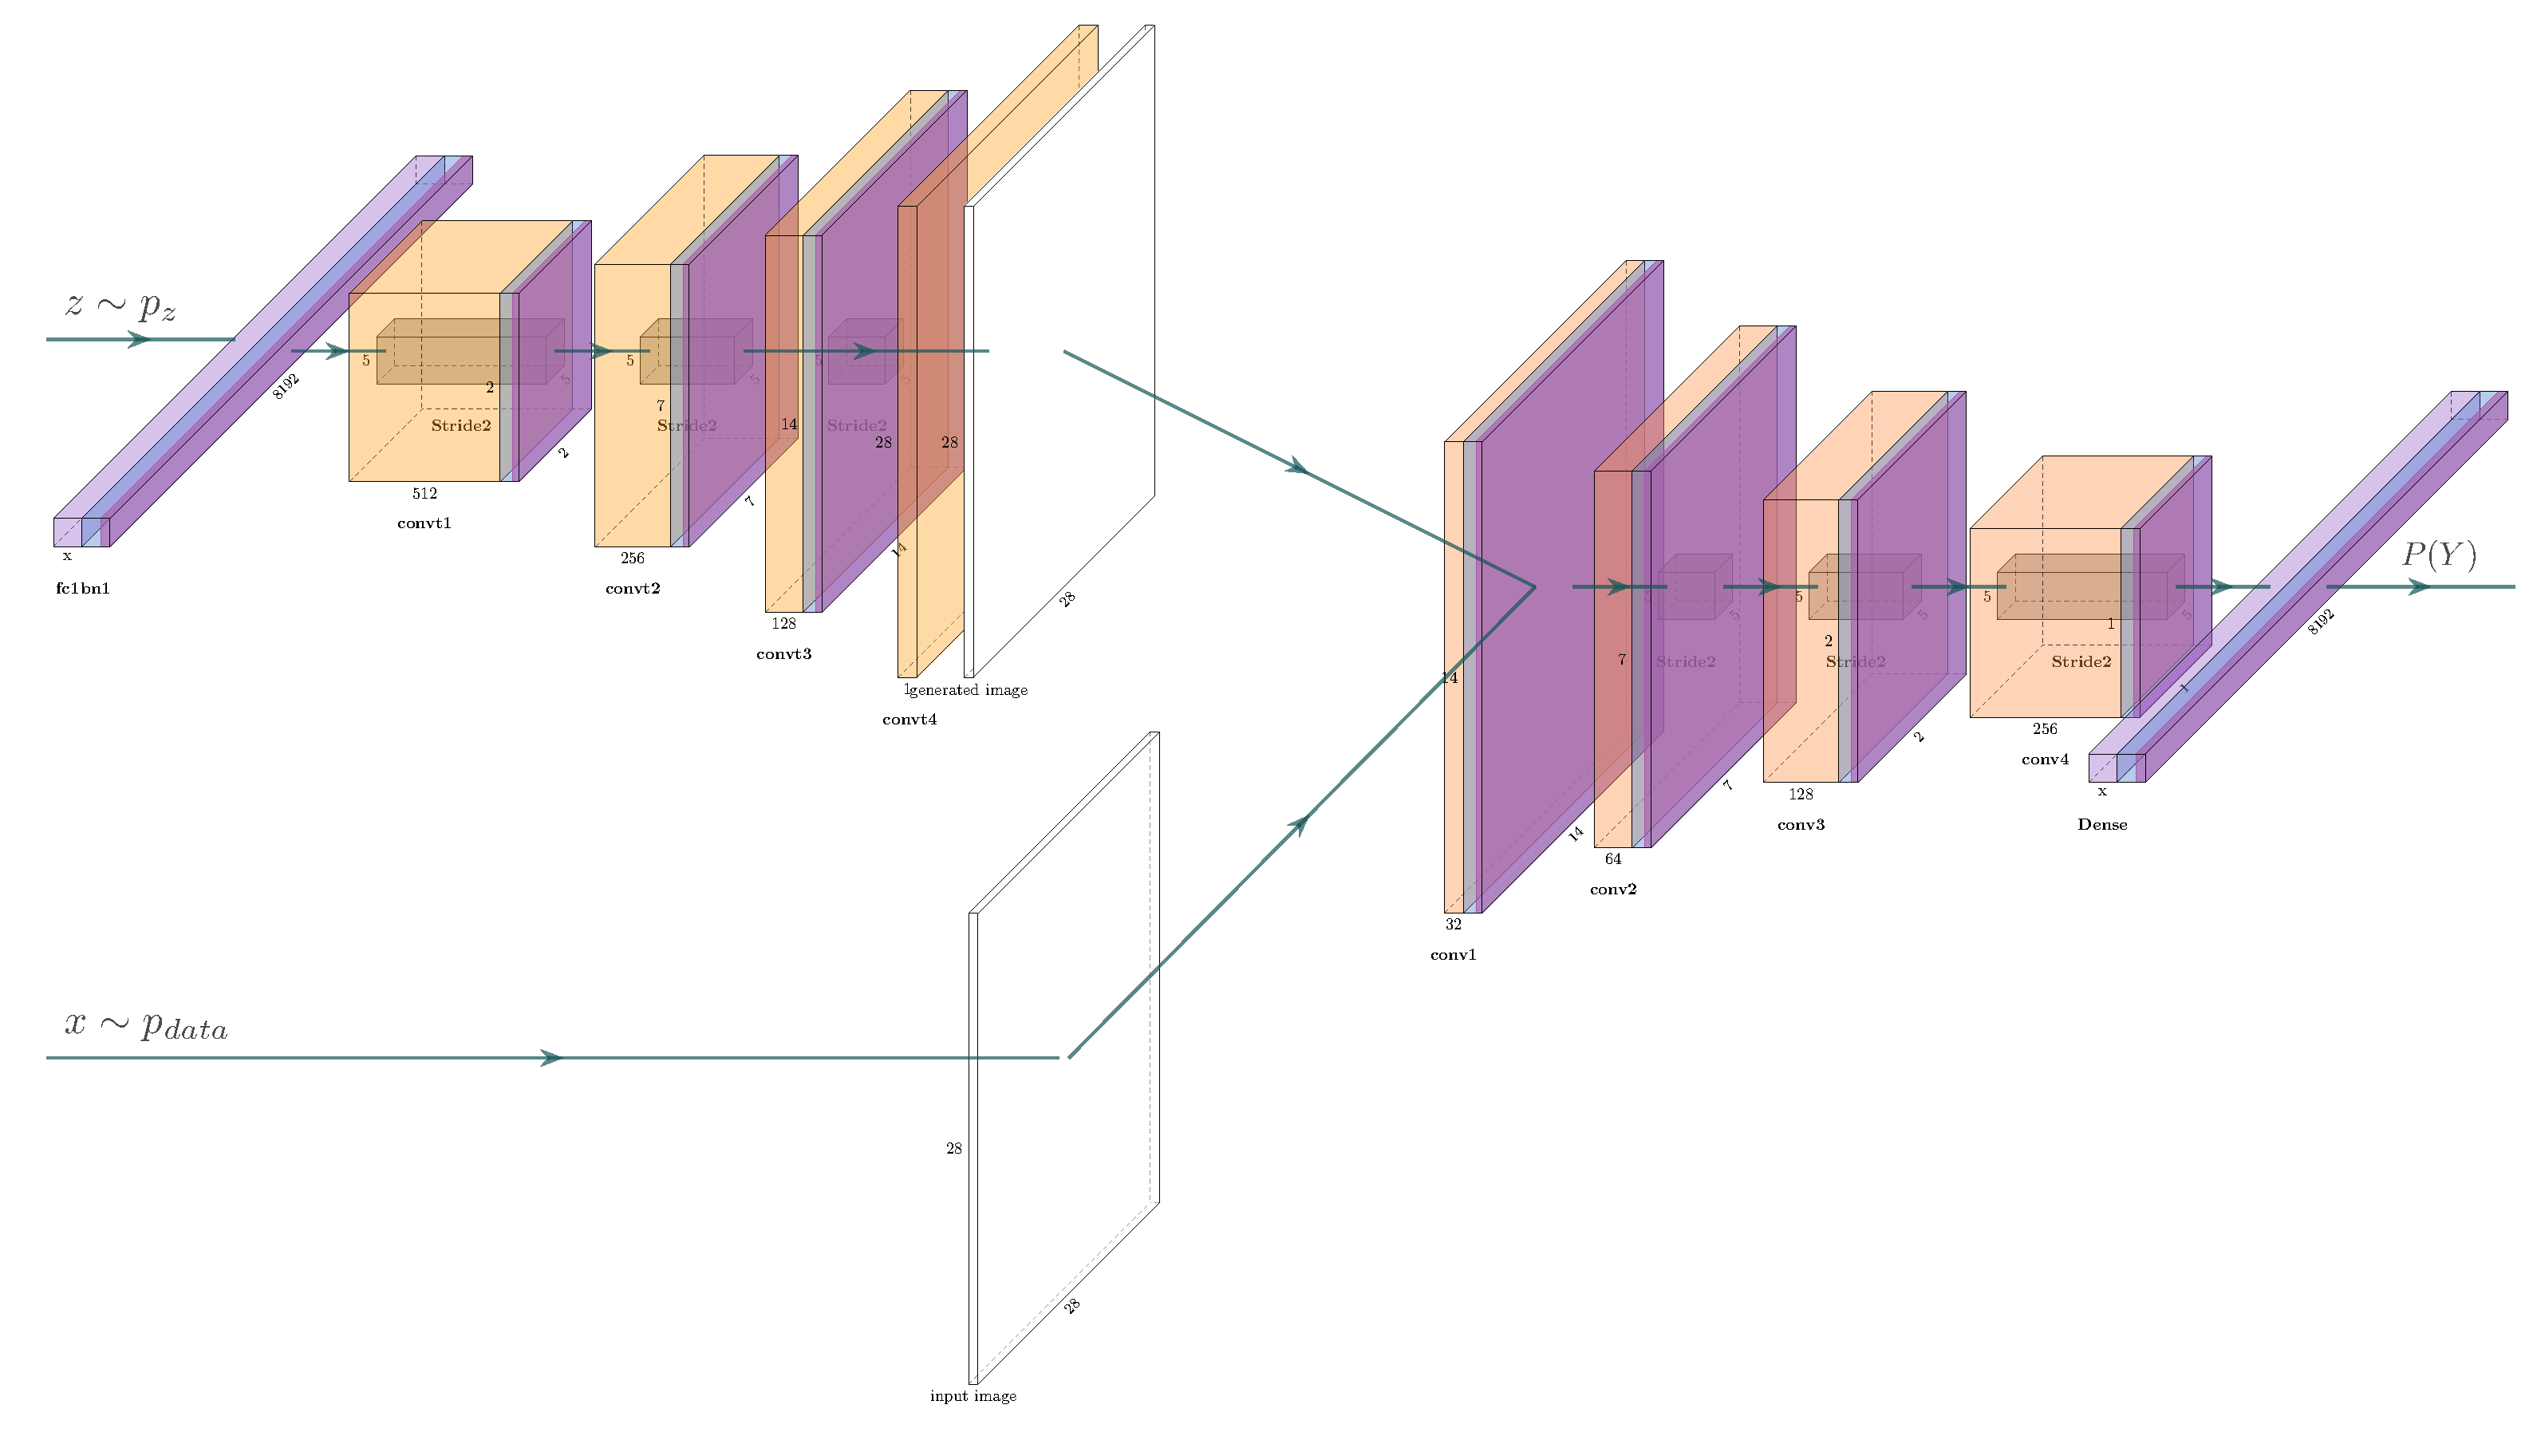
\includegraphics[width=.9\textwidth]{gan}
    \caption{GAN architecture overview}
    \label{fig:gan_network}
\end{figure}

From this point on, "image" will be used to specify the type of the input and the target data because
GAN frameworks are mainly designed to work with high dimensional spatial data like images so it will
be consistent when explaining the theorem and also the central focus of the thesis is on the spatial
data. 

The power of this framework comes from the adversarial nature of the training process. Simply put,
the goal of generator network is to create images similar to the input data by capturing the
data distribution using a probabilistic model. On the other hand discriminator tries to detect fake
(generated) images that is created by generator from the real input images. We can represent this
intuition with the following two player minimax game with the value function $V(G,D)$ in equation \ref{eqn:gan_vgd}.
\cite{Goodfellow:2014:GAN:2969033.2969125}
\begin{align}
    p_{\text{data}} (x) & : x \in \Omega_{X} \quad (\text{Distribution of the data})\\[5pt]
    p_z (z) & : z \in \Omega_{Z} \quad (\text{Distribution of the noise}) \\[5pt]
    \label{eqn:gan_vgd}
    V(G, D) &= \mathbb{E}_{\boldsymbol{x} \sim p_{\text { data }}(\boldsymbol{x})}[\log D(\boldsymbol{x})]+\mathbb{E}_{\boldsymbol{z} \sim p_{\boldsymbol{z}}(\boldsymbol{z})}[\log (1-D(G(\boldsymbol{z})))]
\end{align}

The training objective criterion for the discriminator is to maximize the expected log-likelihood of
classifying the input data as real. $p_{\text{data}}$ represents the distribution of the input.
Since generated data should be classified as fake by the discriminator, the output of the second
term is flipped. The Generator's purpose is to "fool the discriminator". Hence its objective criterion
is to minimize the expected log likelihood of discriminator classifying generated image sample as
fake. We can interpret this equation as two seperate objective functions with different training
criterions :
\begin{align}
    \min _{G} V(G, D)=& \mathbb{E}_{\boldsymbol{z} \sim p_{\boldsymbol{z}}(\boldsymbol{z})}[\log (1-D(G(\boldsymbol{z})))] \\[5pt]
    \max _{D} V(G, D)=& \mathbb{E}_{\boldsymbol{x} \sim p_{\text { data }}(\boldsymbol{x})}[\log D(\boldsymbol{x})]+\mathbb{E}_{\boldsymbol{z} \sim p_{\boldsymbol{z}}(\boldsymbol{z})}[\log (1-D(G(\boldsymbol{z})))]
\end{align}

While this equation describes the relation between two adversaries, it does not provide a
definite explanation how this training objective finds equilibrium and whether that equilibrium also
provides us with the optimal generator or not. For this analysis we will use bottom up approach and
prove the theorem depicted in the original GAN method \cite{Goodfellow:2014:GAN:2969033.2969125}.

\begin{theorem}
\label{thr:gan}
The global minimum of the virtual training criterion $C(G)$ is achieved if and only if $p_g = p_{\text{data}}$.
At that point, $C(G)$ achieves the value $-log(4)$.
\end{theorem} 
We start by defining the term expected value of a function. 

\begin{definition}
    $E(f(x))$ of some function $f(x)$ with respect to  certain probability distribution
$p(x)$ is called the expected value of a function.  
\end{definition}

It is expressed as:
\begin{equation}
    \label{eqn:ev}
    E_{x \sim p_x} = \int p(x) f(x) dx
\end{equation}

So the minimax game equation can be expressed like this: 
\begin{equation}
    \label{eqn:minmax_gan}
    V( G, D) = \int_x p_{\text{data}}(\boldsymbol{x}) log(D(\boldsymbol{x})) dx + \int_z p_z(\boldsymbol{z}) log(1 - D(G(\boldsymbol{z}))) dz
\end{equation}
    
For generator to sample an image good enough to fool the discriminator, framework needs to learn the
implicitly created sample distribution $p_g$ by the generator $G$. Framework defines a prior noise
distribution $z \sim p_z$, isotropic Gaussian distribution with zero mean and unit variance to learn
the distribution $p_g$ (Different distributions are also considered). Next we use the LOTUS theorem.

\begin{theorem}
Law of the unconscious statistician (LOTUS) theorem is used to compute the expected value of a 
function $g(x)$ of a random variable $X$  when one knows the probability distribution of $X$ but 
does not know the probability distribution of $g(x)$. \cite{ringner2009law}
\end{theorem}

The expected value of a function $g(x)$ then can be expressed like:
\begin{equation}
    \mathrm{E}[g(X)]=\sum_{x} g(x) f_{X}(x)  
\end{equation}

$f_{X}(x)$ being the probability distribution of the random variable $X$. 

Using this law we can write the equation $V(G, D)$. 
\begin{align}
    z \sim p_z , \quad G(z) &= x, \quad x \sim p_g\\ 
    V( G, D) &= \int_x p_{\text{data}}(\boldsymbol{x}) log(D(\boldsymbol{x})) + p_g(\boldsymbol{x}) log(1 - D(\boldsymbol{x})) dx
\end{align}

For the Discriminator D, the value of the training criterion should be maximized. That basically means the
function derivative of this expected value expression should be equal to zero. We write the
function by reversing the process of the equation \ref{eqn:ev}.
\begin{align}
    f( p_{\text{data}}, p_g) &= p_{\text{data}}(\boldsymbol{x}) \log(D(\boldsymbol{x})) + p_g(\boldsymbol{x}) \log(1 - D(\boldsymbol{x})) \\[5pt]
    f^{\prime} &= p_{\text{data}}(\boldsymbol{x}) \frac{1}{D(\boldsymbol{x}) \ln(C)} - p_g(\boldsymbol{x}) \frac{1}{(1- D(\boldsymbol{x})) \ln(C)} \\[5pt]
    f^{\prime} &= 0
\end{align}
\begin{align}
    p_{\text{data}}(\boldsymbol{x}) (1- D(\boldsymbol{x})) \ln(C) &= p_g(\boldsymbol{x}) D(\boldsymbol{x}) \ln(C)\\[5pt]
    (p_{\text{data}}(\boldsymbol{x}) +  p_g(\boldsymbol{x})) D(\boldsymbol{x}) &= p_{\text{data}}(\boldsymbol{x})\\[5pt]
    D^{*}_G(\boldsymbol{x}) &= \frac{p_{\text{data}}(\boldsymbol{x})}{(p_{\text{data}}(\boldsymbol{x}) +  p_g(\boldsymbol{x}))}\label{eqn:opt_d}
\end{align}

This is the optimal discriminator $D$ with the fixed $G$. By deriving this value, we show that the
maximum value the Discriminator can reach is the result of the equation \ref{eqn:opt_d}. Next, we reformulate our
$V(G, D)$ to analyze for the training criterion of the generator $G$. 

\begin{align}
    C(G) &= \max _{D} V(G, D) \\[5pt]
    & =\mathbb{E}_{\boldsymbol{x} \sim p_{\mathrm{data}}}\left[\log D_{G}^{*}(\boldsymbol{x})\right]+\mathbb{E}_{\boldsymbol{z} \sim p_{\boldsymbol{z}}}\left[\log \left(1-D_{G}^{*}(G(\boldsymbol{z}))\right)\right] \\[5pt]
    & =\mathbb{E}_{\boldsymbol{x} \sim p_{\mathrm{data}}}\left[\log D_{G}^{*}(\boldsymbol{x})\right]+\mathbb{E}_{\boldsymbol{x} \sim p_{g}}\left[\log \left(1-D_{G}^{*}(\boldsymbol{x})\right)\right] \\[5pt]
    & =\mathbb{E}_{\boldsymbol{x} \sim p_{\mathrm{data}}}\left[\log \frac{p_{\mathrm{data}}(\boldsymbol{x})}{P_{\mathrm{data}}(\boldsymbol{x})+p_{g}(\boldsymbol{x})}\right]+\mathbb{E}_{\boldsymbol{x} \sim p_{g}}\left[\log \frac{p_{g}(\boldsymbol{x})}{p_{\mathrm{data}}(\boldsymbol{x})+p_{g}(\boldsymbol{x})}\right] 
\end{align}

In the theorem, equality $ p_{\text{data}} = p_g$ is given. By applying this equality we get
$D^{*}_G(\boldsymbol{x}) = \frac{1}{2}$. By putting this to our equation we get $$C(G) =
\log(\frac{1}{2}) + \log(\frac{1}{2}) = - \log(4)$$. To verify that this value is indeed the global
point for the equation we apply the following subtraction: 
\begin{multline}
    \label{eqn:gan_optim_proof}
    \begin{split}
        C(G)-(-\log (4))  =\int p_{\text {data}}\left[\log \frac{p_{\text {data}}}{p_{\text {data}}+p_{g}}+\log 2\right]+\\ \int p_{g}\left[\log \frac{p_{g}}{p_{\text {data}}+p_{g}}+\log 2\right]
    \end{split}\\[5pt]
    C(G)-(-\log (4)) =\int p_{\text {data}}\left[\log \frac{2 p_{\text {data}}}{p_{\text {data}}+p_{g}}\right]+\int p_{g}\left[\log \frac{2 p_{g}}{p_{\text {data}}+p_{g}}\right]\\[5pt]
    C(G)-(-\log (4)) =\int p_{\text {data}}\left[\log \frac{p_{\text {data}}}{\left(p_{\text {data}}+p_{g}\right) / 2}\right]+\int p_{g}\left[\log \frac{p_{g}}{\left(p_{\text {data}}+p_{g}\right) / 2}\right]
\end{multline}

To interpret this result we introduce 2 divergence definitions.
\begin{definition}
    The Kullback-Leibler divergence is the measure of how one probability distribution is different from
    the other one.   
\end{definition}
Its general definition is:
\begin{equation}
    D_{K L}(P \| Q)=\int p(x) \log \frac{p(x)}{q(x)}
\end{equation}

More generally if $P$ and $Q$ are probability measures\footnotemark  over a dataset $X$, and measure
$P$ is absolutely continous with respect the $Q$, then the Kullback-Leibler divergence can also be
defined as in equation \ref{eqn:kl}

\footnotetext{A probability measure is a real-valued function defined on a set of events in a probability 
	space that satisfies measure properties such as \textit{countable additivity}\cite{Roussas:1614120}}
\begin{equation}
    \label{eqn:kl}
    D_{\mathrm{KL}}(P \| Q)=\int_{\mathcal{X}} \log \left(\frac{d P}{d Q}\right) d P
\end{equation}

where $\frac{d P}{dQ} (f_{PQ})$ is the Radon-Nikodym derivative \cite{Bill86}. The defining property of
Radon-Nikodym property that ties to the probability measure is that:
\begin{equation}
    \label{eqn:radon}
    P(R) = \int_{R} f_{PQ} d Q
\end{equation}

The RN derivative $f_{PQ} : \Omega \mapsto \mathcal{R}_{\geq 0}$ is defined for any measures $P$ and
$Q$ on a space $\Omega$ such that $P$ is absolutely continous with respect to $Q$. In other words,
for any $ R \subseteq  \Omega : P(R) > 0 \implies Q(R) > 0$ . \cite{Bill86}

Jensen-Shannon divergence is another measure of similarity between different probability
distributions.  Its major difference from the KL divergence is that it is always symmetric and it
always has a non-negative value. The General definition is provided in equation \ref{eqn:jsd}.
\begin{equation}
    \label{eqn:jsd}
    J S D(P \| Q)=\frac{1}{2} D_{K L}(P \| M)+\frac{1}{2} D_{K L}(Q \| M)
\end{equation}

Using this divergence measures we can rewrite our equation as this:
\begin{align}
    \label{eqn:gan_eqaul}
    C(G)&=-\log (4)+K L\left(p_{\text { data }} \| \frac{p_{\text { data }}+p_{g}}{2}\right)+K L\left(p_{g} \| \frac{p_{\text { data }}+p_{g}}{2}\right) \\
    C(G)&=-\log (4)+2 \cdot J S D\left(p_{\text { data }} \| p_{g}\right)
\end{align}

Considering Jensen-Shannon divergence is always non-negative and zero only when the distributions
are identical, we can conclude the proof by stating that the global minimum point of $C^*(G) = -
\log(4)$ is only achieved when $p_{\text{data}} = p_g$ .

Intuition behind the adversarial training of this framework is important because all the subsequent
approaches that will be discussed in the thesis that use GAN's fundamentally benefit from this
framework to train their networks. As we will see in the BiGAN (section \ref{sec:bigan}) and similar models, addition of
encoder network changes the overall minimax game played by the adversary networks but underlying
logic still depends on the value function of the GANs.

\subsection{Autoencoder Networks}
\label{sec:ae}
 
Autoencoder network is a type of neural network that is trained to copy its input data to output.
\cite{Goodfellow-et-al-2016} In its simplest form, it can be defined as a feedforward, non-
recurrent network similar to multilayer perceptrons like in figure \ref{fig:ae_simple}.
\begin{figure}[h!]
	\centering
	\includegraphics[width=.75\textwidth]{ae_simple}
    \caption{Simple Autoencoder architecture}
    \label{fig:ae_simple}
\end{figure}
Internally, it consists of a hidden layer that describes the representation (code) learned from the
input data. Connections from the hidden layer to the output layer transforms the hidden
representation into the output data with the same dimensionality as the input. Rather that trying to
reconstruct the given data, autoencoders are mainly used to learn the representation about the data
to extract meaningful features and to reduce the dimensionality of data while keeping the
relevant information as an alternative to principal component analysis. 

\begin{figure}[h!]
	\centering
	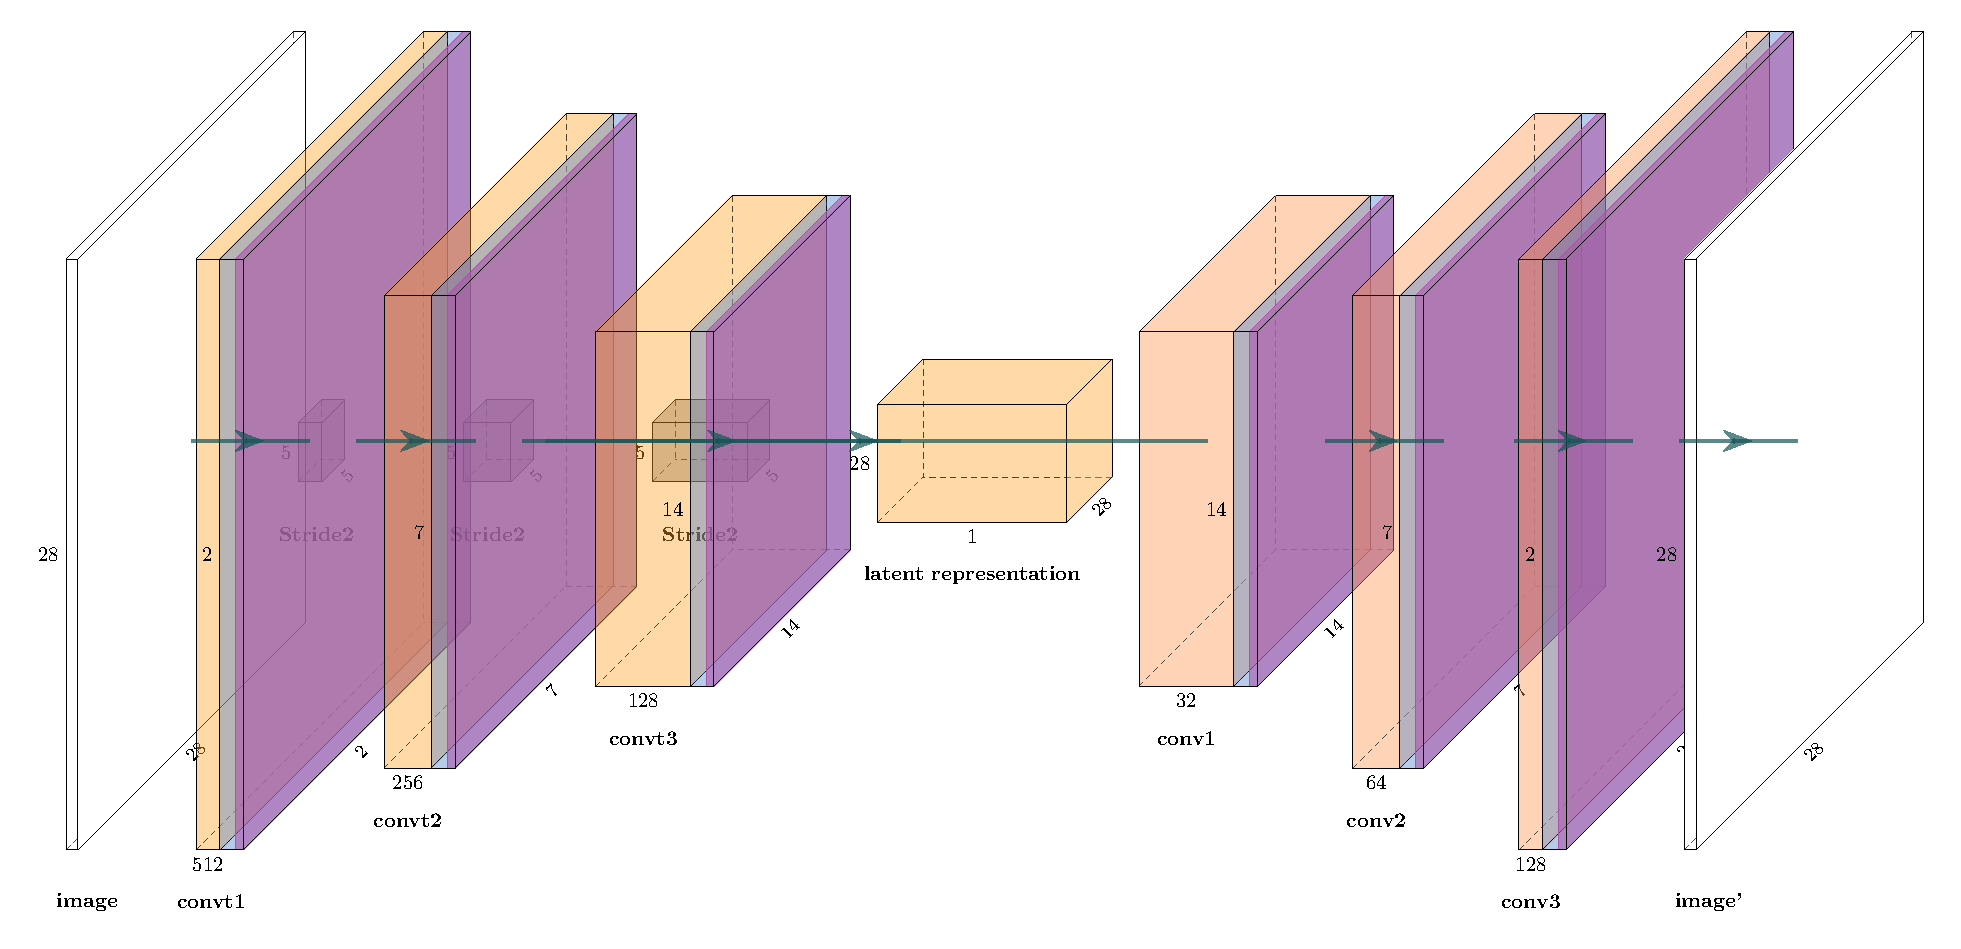
\includegraphics[width=.9\textwidth]{autoencoder}
    \caption{Stacked Autoencoder with multiple layers}
    \label{fig:ae_deep}
\end{figure}

With the increased complexity of the data present, this architecture can be extended to capture more
complex feature representations by stacking similar but varying encoder and decoder layers on top of
each other. Generally first layers learn the more basic features of the data and as the layers are
stacked, more concentrated and complex features can be learnt in the code section of the
autoencoder, end of the encoder network. These architectures are mainly referred to as deep
autoencoders because of the increased level of hidden layers present in the model depicted in figure
\ref{fig:ae_deep}, just like in deep learning.

Learning rationale of the autoencoders can be visualized with a pair of weighted layer computation
functions like in the multilayer perceptrons. Assume that we have two transition functions that
defines the relationship between the real data and the intermediate representation as the result of
the encoder network:
\begin{align*}
    \phi : X \mapsto F \\
    \psi : F \mapsto X     
\end{align*}

We can define the intermediate representation computation and the reconstruction of input data
with the following equations:
\begin{align}  
    z  &= \sigma( W x + b) ,\quad x \sim X \in \mathbb{R}^d ,\quad z \sim F \in \mathbb{R}^p \\
    x'  &= \sigma' (W' z + b') 
\end{align}

The primal training objective for the autoencoders is the reconstruction loss. Depending on the
architecture of the decoder or the desired task, the source of parameters for the objective
function can change. Autoencoder learns the representation of data by minimizing the objective function 
defined as the reconstruction loss. 
\begin{align}
    \label{eqn:ae_rec}
  \phi, \psi & = \underset{\phi, \psi}{\text{argmin}} \norm{X - (\psi \circ \phi) X} \\  
  L(x, x') & = \norm{x - x'}^2 = \norm{x - \sigma' (W' \sigma (W x + b) + b')}^2
\end{align}

With enough model capacity and training time, autoencoder might learn to copy the input perfectly.
This reduces the functionality of the encoder-decoder modules to a identity function:
$$
 x \sim X \in \mathbb{R}^d, \quad \psi(\phi(x)) = x
$$

This is generally an unwanted outcome. To overcome this problem, autoencoders are designed to learn the
representation of the data imperfectly. \cite{Goodfellow-et-al-2016} This is achieved by how the
encoder module learns to compress the data to a meaningful representation. These 3 types of
autoencoder models can give an idea about how the architecture can be changed to alter the amount of
information that can be extracted from the data. These are:

\begin{itemize}
    \item Undercomplete Autoencoders
    \item Regularized Autoencoders
    \item Denoising Autoencoders
    %\item Variational Autoencoders
\end{itemize}

Undercomplete autoencoders reduce the dimension size of the latent representation. Learning
purposefully insufficient representation forces autoencoder to keep the most salient features about
the data. Training objective function is the reconstruction loss which presented in equation
\ref{eqn:ae_rec}. If the computation of this function is linear, then the autoencoder mimics the
behaviour of a principal component analysis method. When the encoder transition $\phi$ and the
decoder transition $\psi$ is designed to have a nonlinear nature, then the autoencoder has the
ability to capture more complex reprensetation of the data, more powerful approach than known dimensionality 
reduction methods such as Principal Component Analysis. But this has the risk of again, causing 
autoencoder to replicate the input data perfectly and becoming an identity function $x' = \psi(\phi(x))$. 
Regularized autoencoders' design difference is that their latent representation layer usually has same 
or higher dimensional power (more neurons from the perspective of multilayer perceptrons). 
To acquire a similar performance like undercomplete variants, they regularize the loss function  
with the potential properties of the data distribution such as robustness to the noise or the 
sparsity of the representation. Prioritizing which aspects of the data will be used as a regularizer 
term for the objective function is a task dependent problem. \cite{Goodfellow-et-al-2016}. 
Denoising autoencoders tries to solve a different problem to achieve a good representation. 
$$
\hat{x} = x + \epsilon : x \sim X \in \mathbb{R}^d ,\quad \epsilon \sim \mathcal{N}(\mu, \sigma^2)
$$

The input data is corrupted with some kind of noise, gaussian etc. Denoising autoencoders tries to
reconstruct the data and undo this corruption by minimizing this updated loss with the difference of
$\hat{x}$
$$
L(x, \psi(\phi(\hat{x})))
$$

In the remaining part of this thesis, these networks will be referenced several times. They constitute the 
building blocks of all the models presented in the next section. Our proposed model's architecture also structured 
using these networks so their underlying logic is fundamental to understand to compose our solution.

\section{GAN Based Anomaly Detection Methods}
\label{sec:gan_based_sota}
In the field of reconstruction based anomaly detection, autoencoder architectures 
are fairly popular with spatial data \cite{baldi2012autoencoders,leveau2017adversarial,an2015variational}.
GAN based approaches in this field are relatively new compared to their other variants.
In the following subsections, we will explain the approaches that can be considered as the state of
the art for this problem in the order of their complexity and incremental improvements. Each
approach will be evaluated by their problem description, the type of data they use, model
architecture and anomaly score computation. 

\subsection{AnoGAN}
\label{sec:anogan}
 AnoGAN model is the first approach that utilizes GANs for the anomaly detection task.
\cite{Schlegl2017UnsupervisedAD} It focuses on the problem of detecting anomalous regions in optical
coherence tomography images. Images containing retinal fluid or hyperreflective foci (indicator of
disease progression in various retinal diseases) are identified as anomalous examples. The main
motivation to use GANs to obtain a model which represents normal anatomical variability of the data
is that previous supervised approaches involves training a model with a large dataset using
annotated examples of known markers. Relying on vocabulary of markers may limit the predictive power
of the model as the image contains much more relevant information than the marker and extensive
supervised training is a problem because it means that every stage of the disease requires an
extensive training with annotated examples such as labeled lesions which may decrease limit of
exploiting imaging data for treatment decisions. \cite{Schlegl2017UnsupervisedAD}.


The framework consists of 2 parts. First part is the GAN module, generator and discriminator
networks (see figure \ref{fig:gan_network}). Their architecture is inspired by the original DCGAN
\cite{Radford2016UnsupervisedRL} which contains convolutional layers instead of multi layer perceptron 
layers. The objective function of the GAN is the same of the equation \ref{eqn:gan_vgd}. 
During the training the generator enhances its ability to generate more realistic
retinal images while the discriminator learns the diagnose the real and the generated sample more
efficiently. 

The second part of the framework is about the inverse mapping of the noise to the image. We know
from the GANs training procedure that when the adversarial training is completed, the generator
network has learned the distribution $p_g$ that is theoretically very similar to the input data
distribution $p_{\text{data}}$. ( I state "theoretically" explicitly because depending on the
configuration of GAN and the data that is used, this may differ significantly in practice. This
aspect of the learning will be mentioned in the latter approaches.) Even though with the trained
generator, 
$$
G(z) = z \mapsto x,x \sim p_{\text{data}}
$$

the GAN framework does not learn the inverse mapping from the image to noise. AnoGAN framework
aims to find the noise sample $z\prime$ from the query image (normal or anomalous) such that the
generated image $G(z\prime)$ is visually the most similar one to the query image. This is essential
for the anomaly detection task. $z\prime$ is sampled randomly as initialization. Then the
$G(z\prime)$ is computed and based on the defined loss function gradients the coefficients of
$z\prime$ is updated using back propagation. This procedure is repeated for a number of epochs to
obtain the final value of the $z\prime$. 

The loss function for the inverse mapping is defined as the combination of two separate losses.
Residual loss is responsible for enforcing visual similarity between the generated image
$G(z\prime)$ and the query image $x$.
\begin{equation}
    \label{eqn:anogan_rl}
    L_R (z_{\gamma}) = \sum \norm{ x - G(z_{\gamma})}
\end{equation} 
Discrimination loss on the other hand enforces the
generated image $G(z\prime)$ to lie on the manifold $X$ of image $x$.
\begin{equation}
    \label{eqn:anogan_dl}
    L_D (z_{\gamma}) = \sum  \norm{f(x) - f(G(z_{\gamma})}
\end{equation}

There are two different implementation for the discrimination loss. One with sigmoid cross entropy
which is from the original GAN implementation \cite{Goodfellow:2014:GAN:2969033.2969125} and one
with feature matching \cite{fm} which uses the last layer of the discriminator rather than the
output to compute the loss. Using this loss allows them to use discriminator not as a classifier but
as a feature extractor. Using both residual and discrimination loss, the total loss function is
defined as :
$$L(z_{\gamma}) = (1 - \lambda ) \times L_{R}(\boldsymbol{z_{\theta}}) + \lambda \times
L_{D}(\boldsymbol{z_{\gamma}})$$

Only the coefficients of $z$ is adapted via back propagation. The trained weights of the generator
and discriminator are fixed in this stage. \cite{Schlegl2017UnsupervisedAD}

Anomaly detection task uses same loss functions to compute the anomaly score. 
$$A(x) = (1 - \lambda ) \times R(\boldsymbol{x}) + \lambda \times D(\boldsymbol{x}) $$

The $R(x)$ is the residual score value and the $D(x)$ is the discrimination score value at the last
update iteration of the inverse mapping procedure, respectively. The model outputs a larger anomaly
score $A(x)$ for anomalous samples though smaller score means that very similar image is seen during
the training of GAN. 

This model is the first model that integrates generative adversarial networks to an anomaly
detection framework. The mapping from latent representation to image data is completely dependent on
the architecture of GAN and its training parameters. The disadvantageous aspect of this approach
is the inference. For each query image framework approximates the latent representation vector using
back propagation steps which makes the whole process significantly slow compared to the other
approaches. Improvements to this framework is discussed in the Latest Developments chapter
(\ref{sec:fanogan}). The experiment results and the implementation details will be covered in
chapter \ref{chap:expres}.

\subsection{BiGAN and ALI}
\label{sec:bigan}

 BiGAN ( Bidirectional Generative adversarial Networks) \cite{Donahue2017AdversarialFL} and ALI
 (Adversarially Learned Inference) \cite{Dumoulin2017AdversariallyLI} are two models that
 independent from each other but focuses on the same problem. They investigate to acquire efficient
 inference method from data to latent space by using encoders in the adversarial training framework
 of GANs. They emphasize learning the inverse mapping for the auxiliary supervised tasks such as
 classification, segmentation and discrimination. The only difference between the models is that the
 BiGAN uses a deterministic network for the encoder while ALI uses a stochastic network. I will
 first briefly explain the original architecture of the ALI and continue to present the framework in
 detail using BiGAN instead since their explanation for the model is more consistent with the GAN
 framework. Furthermore I will discuss how this architecture can be used for anomaly detection. In
 the original papers, anomaly detection has not been explored as an auxilary supervised task but the
 later models like in section \ref{sec:alad} or in section \ref{sec:ganomaly}, used these
 architectures as a state of the art comparison in terms of both foundation and performance measure
 hence their use of anomaly detection will also be discussed.

\begin{figure}[h!]
	\centering
	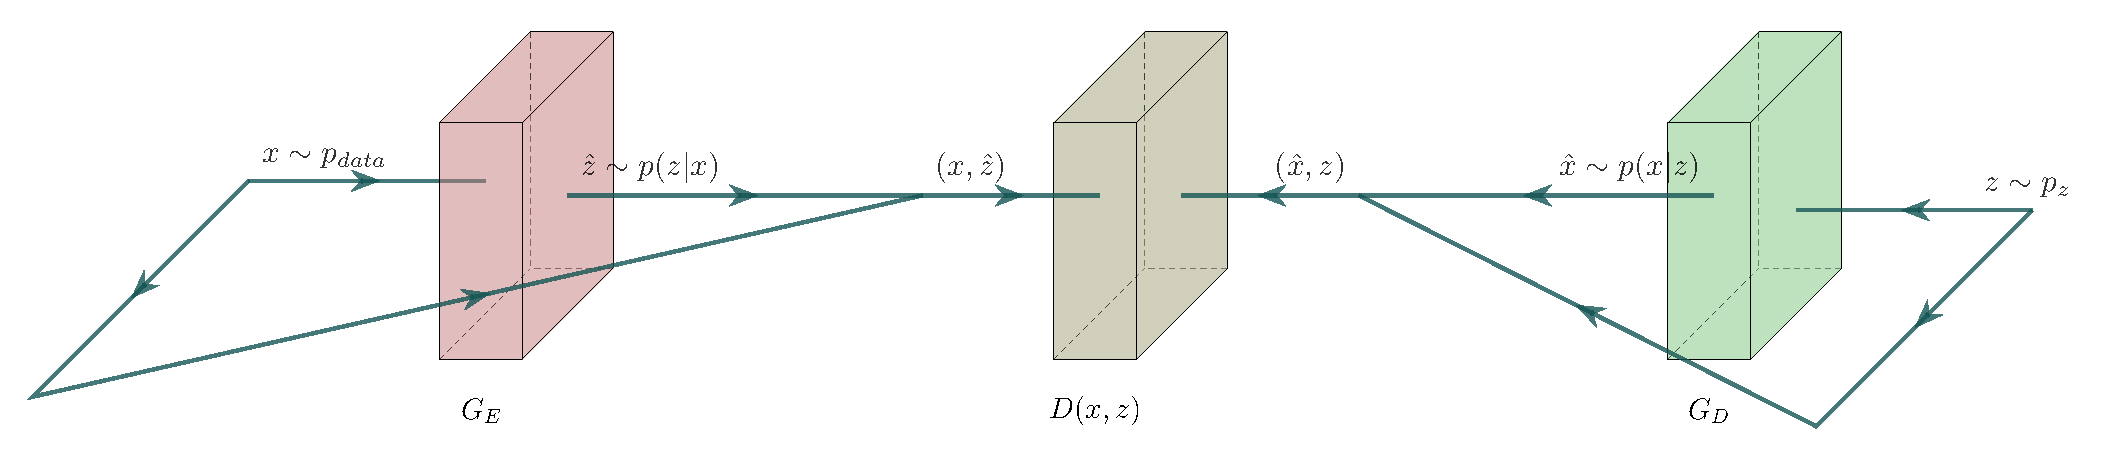
\includegraphics[width=.9\textwidth]{aligan}
    \caption{ALI architecture overview}
    \label{fig:aligan_model}
\end{figure}

Aligan architecture is depicted as a generator and a discriminator in figure \ref{fig:aligan_model}.
The significant change in ALI is that the generator is the combination of decoder network and an
encoder network. Encoder represents the joint distribution $p_{E}(x, z)$ which has the marginal
$p_{\text{data}(x)}$ and decoder represents the joint distribution $p_{D}(x, z)$ with the marginal
$p_z(z)$ which represents the factorized noise distribution (generally $\mathcal{N}(0, 1)$). The
objective function of the ALI is to match these two joint distributions. Successing in this goal
also ensures the match of marginals and conditional distributions $p(z | x)$ and $p(x | z)$
. Discriminator is also modified to support this new objective function. It is trained to
distinguish between the joint pairs  $(x, \hat{z} = G_{E}(x))$ and $(\hat{x} = G_{D}(z), z)$ as data
and noise.

\begin{figure}[h!]
	\centering
	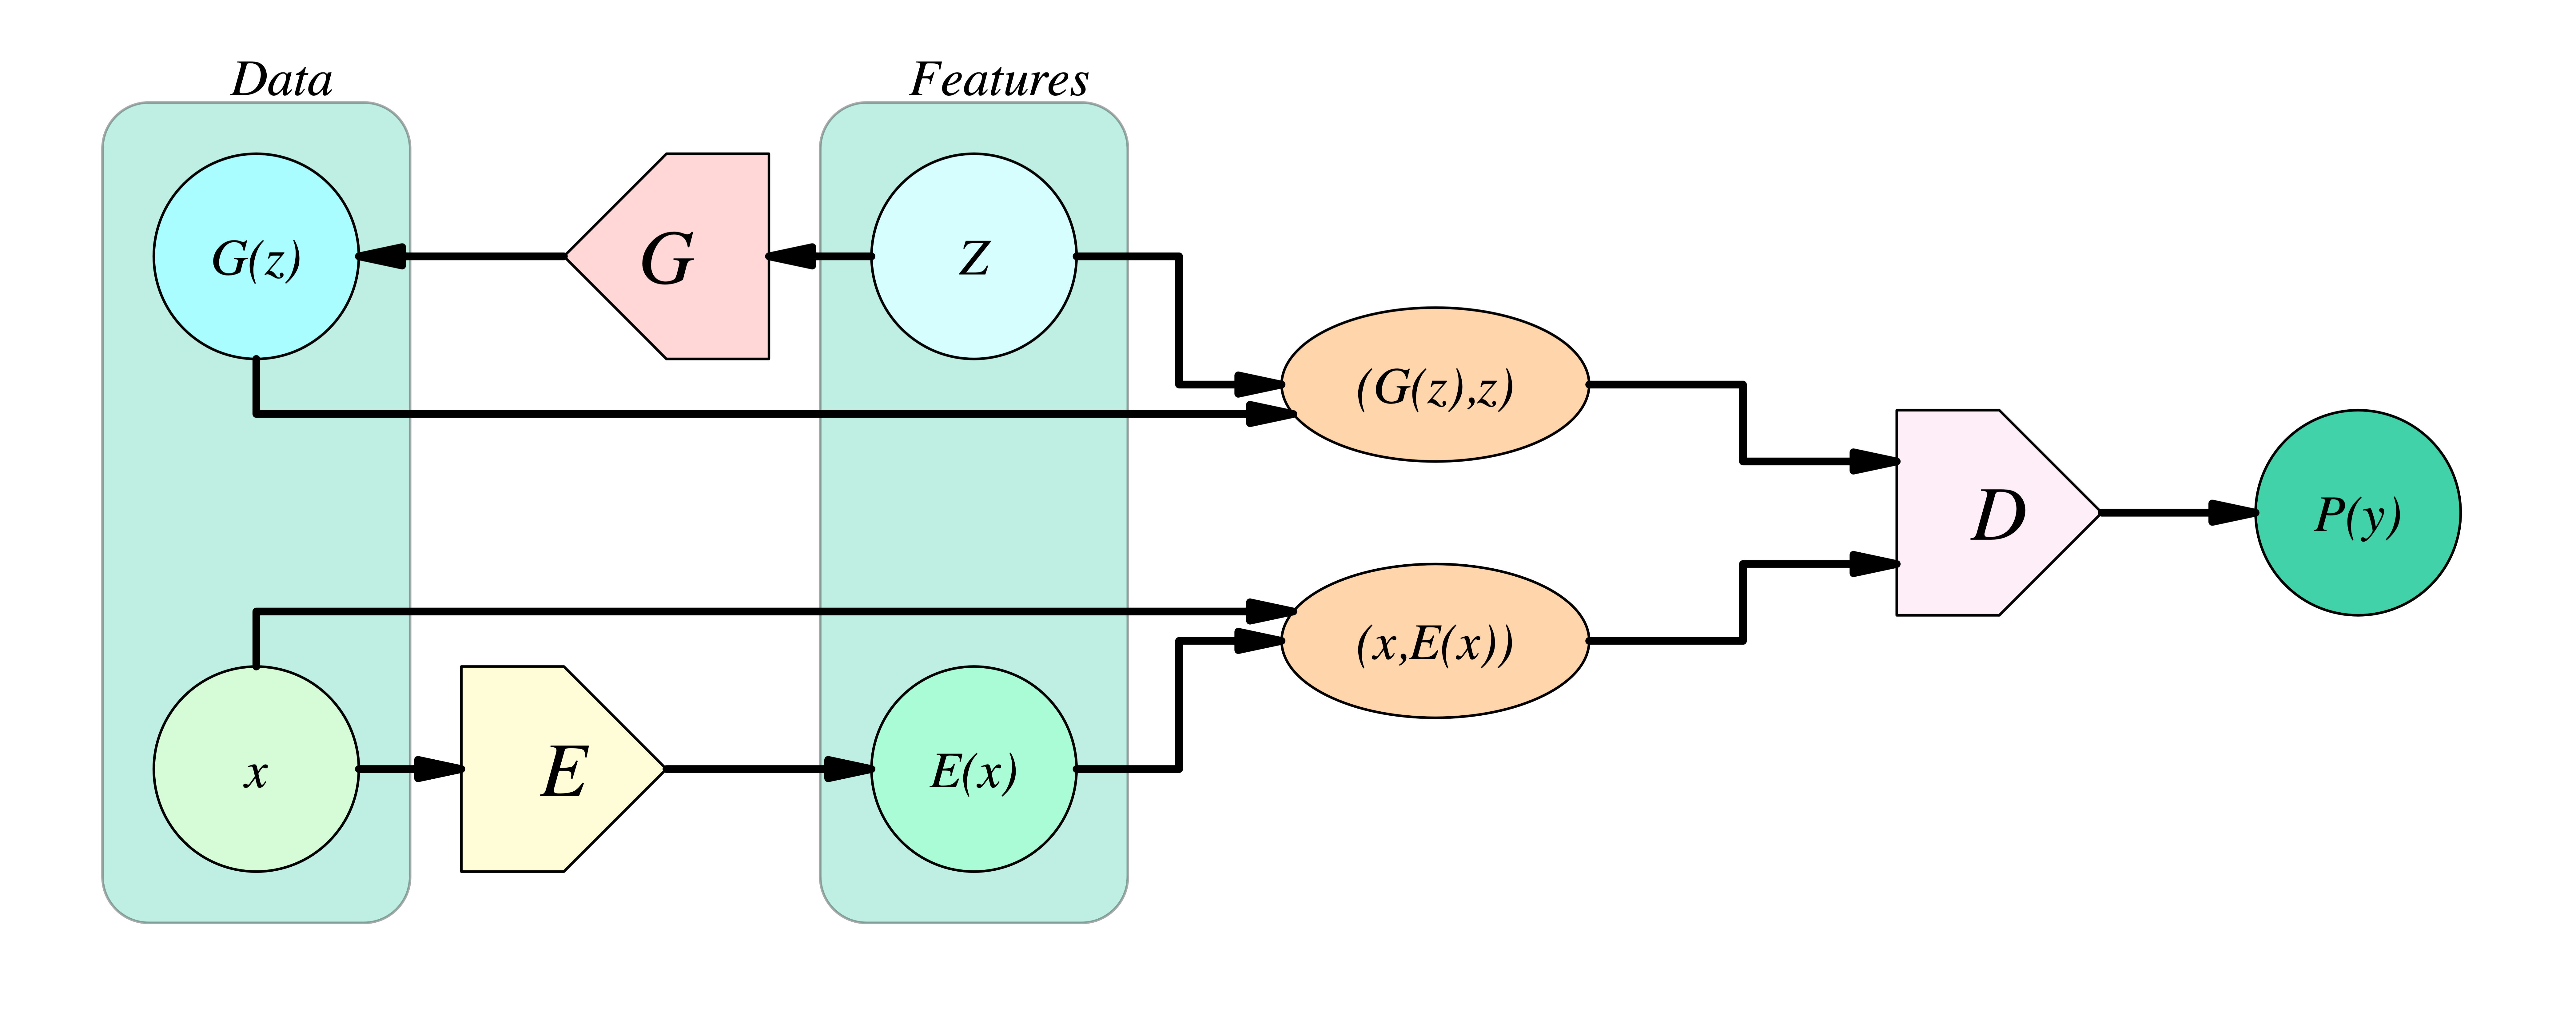
\includegraphics[width=.9\textwidth]{bigan}
    \caption{BiGAN architecture overview}
    \label{fig:bigan_model}
\end{figure}

% TODO stochastic deterministic farkini bir cumle ile acikla.
BiGAN architecture model is presented in figure \ref{fig:bigan_model}. The architectures are
theoretically identical with the exception of the encoder network choice in practise. BiGAN
experiments are conducted with a deterministic network whilst ALI framework used a stochastic
network. Apart from the generator, BiGAN also trains the encoder network in an adversarial manner.
Same objective function used in GAN provides the relationship between the generator and encoder that
$G = E^{-1}$ and vice versa. This invertibility is the key aspect of the model and other
frameworks to provide an efficient inference with reliable sampling. We Know from the section
\ref{sec:gan} that: 
$$
G : \Omega_{z} \mapsto \Omega_{x}
$$

We define the Encoder with reverse of that transition:
$$
E : \Omega_{x} \mapsto \Omega_{z}
$$

Since this framework accepts the networks as deterministic we also redefine the distributions for
generator and encoder networks:
\begin{align*}
    p_G(x | z) & = \delta (x - G(z)) \\
    p_E(z | x) & = \delta (z - E(x))
\end{align*}

The objective function of the framework can be characterized as:
\begin{equation}
    \min _{G, E} \max _{D} V(D, E, G)
\end{equation}
 
where
\begin{multline}
    \label{eqn:bigan_v}
V(D, E, G) :=\mathbb{E}_{\mathbf{x} \sim p_{\mathbf{X}}}  \underbrace{\left[ \mathbb{E}_{\mathbf{z} \sim p_{E}(\cdot | \mathbf{x})}[\log D(\mathbf{x}, \mathbf{z})] \right]}_{\log D(\mathbf{x}, E(\mathbf{x}))} + \\ \mathbb{E}_{\mathbf{z} \sim p_{\mathbf{Z}}} \underbrace{  \left[ \mathbb{E}_{\mathbf{x} \sim p_{G}(\cdot | \mathbf{z})}[\log (1-D(\mathbf{x}, \mathbf{z}))] \right]}_{\log (1-D(G(\mathbf{z}), \mathbf{z}))}
\end{multline}

To prove that the encoder is the inverse of the generator, optimal discriminator needs to be
determined.\cite{Donahue2017AdversarialFL} The joint distributions of the generator and encoder can
be illustrated as the marginals of the data and noise and related conditional probability
distributions:
\begin{align}
    \label{eqn:bigan_gz}
    p_{GZ} (x, z ) &:= p_G(x | z) p_{Z} (z) \\[5pt] 
    \label{eqn:bigan_ex}
    p_{EX} (x, z ) &:= p_E(z | x) p_{X} (x) 
\end{align}

The joint latent space and the data for the problem can also be illustrated as a joint
representation.
$$
\Omega := \Omega_{X} \times \Omega_{Z}
$$

For the region $R \subseteq \Omega$ probability
measures\cite{RePEc:eee:csdana:v:20:y:1995:i:6:p:703-702} of encoder and generator is defined in
equation \ref{eqn:prob_measure1} and \ref{eqn:prob_measure2} respectively.\cite{Donahue2017AdversarialFL}

 \begin{align}
    \begin{split}\label{eqn:prob_measure1}
    P_{E \mathbf{X}}(R)  :={}&\int_{\Omega} p_{E \mathbf{X}}(\mathbf{x}, \mathbf{z})
    \mathbf{1\footnotemark}_{[(\mathbf{x}, \mathbf{z}) \in R]} \mathrm{d}(\mathbf{x}, \mathbf{z})= \\ 
    & \quad \int_{\Omega \mathbf{x}} p_{\mathbf{X}}(\mathbf{x}) \int_{\Omega \mathbf{z}} p_{E}(\mathbf{z} | \mathbf{x})
    \mathbf{1}_{[(\mathbf{x}, \mathbf{z}) \in R]} \mathrm{d} \mathbf{z} \mathrm{d} \mathbf{x}       
    \end{split}\\
    {}&=\int_{\Omega_{\mathbf{X}}} p_{\mathbf{X}}(\mathbf{x})\left(\int_{\Omega_{\mathbf{Z}}} \delta(\mathbf{z}-E(\mathbf{x})) \mathbf{1}_{[(\mathbf{x}, \mathbf{z}) \in R]} \mathrm{d} \mathbf{z}\right) \mathrm{d} \mathbf{x} \\[5pt]
    {}& =\int_{\Omega_{\mathbf{X}}} p_{\mathbf{X}}(\mathbf{x}) \mathbf{1}_{[(\mathbf{x}, E(\mathbf{x})) \in R]} \mathrm{d} \mathbf{x} \\[5pt]
    \begin{split}\label{eqn:prob_measure2}
    P_{G \mathbf{Z}}(R) :={}&\int_{\Omega} p_{G \mathbf{Z}}(\mathbf{x}, \mathbf{z}) 
    \mathbf{1}_{[(\mathbf{x},\mathbf{z}) \in R]} \mathrm{d}(\mathbf{x}, \mathbf{z})= \\ 
    & \quad \int_{\Omega_{\mathbf{Z}}} p_{\mathbf{Z}}(\mathbf{z}) \int_{\Omega_{\mathbf{X}}} p_{G}(\mathbf{x} | \mathbf{z})
    \mathbf{1}_{[(\mathbf{x}, \mathbf{z}) \in R]} \mathrm{d} \mathbf{x} \mathrm{d} \mathbf{z} 
    \end{split}\\
    {}&=\int_{\Omega_{\mathbf{Z}}} p_{\mathbf{Z}}(\mathbf{z})\left(\int_{\Omega_{\mathbf{X}}} \delta(\mathbf{x}-G(\mathbf{z})) \mathbf{1}_{[(\mathbf{x}, \mathbf{z}) \in R]} \mathrm{d} \mathbf{x}\right) \mathrm{d} \mathbf{z} \\[5pt]
    {}& =\int_{\Omega_{\mathbf{Z}}} p_{\mathbf{Z}}(\mathbf{z}) \mathbf{1}_{[(G(\mathbf{z}), \mathbf{z}) \in R]} \mathrm{d} \mathbf{z}
\end{align}        
\footnotetext{ Indicator function is a type of characteristic function that is used to indicate a
membership on a subset $X$. It is denoted with bold \textbf{1} symbol.}  

Probability measures over regions on the image data $R_X \subseteq \Omega_{X}$ and the latent noise
$R_Z \subseteq \Omega_{Z}$ can be similarly defined.

\begin{align}
    P_{\mathbf{X}}\left(R_{\mathbf{X}}\right) :=&\int_{\Omega_{\mathbf{X}}} p_{\mathbf{X}}(\mathbf{x}) \mathbf{1}_{\left[\mathbf{x} \in R_{\mathbf{X}}\right]} \mathrm{d} \mathbf{x} \\[5pt]
    P_{\mathbf{X}}\left(R_{\mathbf{X}}\right) :=&\int_{\Omega_{\mathbf{X}}} p_{\mathbf{X}}(\mathbf{x}) \mathbf{1}_{\left[\mathbf{x} \in R_{\mathbf{X}}\right]} \mathrm{d} \mathbf{x}
\end{align}

The optimal discriminator follows the same derivation from the GAN framework
\cite{Goodfellow:2014:GAN:2969033.2969125}. The Objective equation \ref{eqn:bigan_v} can be reduced
to the Jensen-Shannon divergence between joint distributions $P_{E\mathbf{X}}$ and $P_{G\mathbf{Z}}$
with the proof of the following propositions from the BiGAN \cite{Donahue2017AdversarialFL}.

\begin{prop}
    \label{prop:bigan_1}
    For any $E$ and $G$, the optimal discriminator $D^*_{EG} := \\ \underset{D}{\text{argmax}}  V(D, E,
    G)$ is the Radon-Nikodym derivative $f_{EG} := \frac{dP_{E\mathbf{X}}}{dP_{E\mathbf{X}} +
    dP_{G\mathbf{Z}}}  : \Omega  \mapsto [0, 1]$ of measure $P_{E\mathbf{X}}$ with respect to measure
    $ dP_{E\mathbf{X}} + dP_{G\mathbf{Z}}$.
\end{prop}

\begin{prop}
    \label{prop:bigan_2}
  The encoder and generator's objective for an optimal discriminator $C(E, G):= \underset{D}{max}
  V(D, E, G) = V(D^*_{EG}, E, G)$ can be rewritten in terms of the Jensen-Shannon divergence between
  the measures $P_{EX}$ and $P_{GZ}$ as $C(E, G) = 2 D_{JS} (P_{E\mathbf{X}} \parallel P_{G\mathbf{Z}}) -
  \log 4$    
\end{prop}

Discriminator is trained with both the encoder and generator network output. Therefore it is
rational to assume that if we were to define a probability measure for discriminator . So we let $P_{EG}$
be the average of $P_{E\mathbf{X}}$ and $P_{G\mathbf{Z}}$. 
\begin{equation}
  P_{EG} = \frac{P_{E\mathbf{X}} + P_{G\mathbf{Z}}}{2}  
\end{equation}

Since both $P_{E\mathbf{X}}$ and $P_{G\mathbf{Z}}$ are continuous with respect to the $P_{EG}$, the
relationship of RN derivatives of $f_{EG}$ and $f_{GE}$ is defined accordingly:
\begin{align}
  f_{EG} :=& \frac{ d P_{E\mathbf{X}} }{ d P_{E\mathbf{X}} + d P_{G\mathbf{Z}}} \\[5pt]
  f_{GE} :=& \frac{ d P_{G\mathbf{Z}} }{ d P_{E\mathbf{X}} + d P_{G\mathbf{Z}}} \\[5pt]
  f_{EG} + f_{GE} :=   \frac{ d P_{G\mathbf{Z}} }{ d P_{E\mathbf{X}} + d P_{G\mathbf{Z}}} &+ \frac{ d P_{E\mathbf{X}} }{ d P_{E\mathbf{X}} + d P_{G\mathbf{Z}}} = \frac{ d( P_{G\mathbf{Z}} + P_{E\mathbf{X}}) }{ d( P_{G\mathbf{Z}} + P_{E\mathbf{X}} ) } = 1 
\end{align}

Using the property of RN derivative (equation \ref{eqn:radon}) we can transform the expected value
function and rewrite the objective function of the BiGAN with a single probability
measure.\cite{Donahue2017AdversarialFL} \cite{Goodfellow:2014:GAN:2969033.2969125}
\begin{equation}
    \label{eqn:transform}
    \mathbb{E}_{\mathbf{x} \sim P}[g(\mathbf{x})]=\int_{\Omega} g \mathrm{d} P=\int_{\Omega} g \frac{\mathrm{d} P}{\mathrm{d} Q} \mathrm{d} Q=\int_{\Omega} g f_{P Q} \mathrm{d} Q=\mathbb{E}_{\mathbf{x} \sim Q}\left[f_{P Q}(\mathbf{x}) g(\mathbf{x})\right]
    %\caption{expression change of expected value computation with a different distribution}
\end{equation}
We start by rewriting the original objective function with the joint probability distributions.
\begin{equation}
    V(D, E, G) = \mathbb{E}_{(\mathbf{x}, \mathbf{z}) \sim P_{E \mathbf{X}}}[\log D(\mathbf{x}, \mathbf{z})]+\mathbb{E}_{(\mathbf{x}, \mathbf{z}) \sim P_{G \mathbf{Z}}}[\log (1-D(\mathbf{x}, \mathbf{z}))] 
\end{equation}

Then the transformation described in equation \ref{eqn:transform} is applied.
\begin{equation}
    =\mathbb{E}_{(\mathbf{x}, \mathbf{z}) \sim P_{E G}}  [ \underbrace{2 f_{E G}}_{\frac{\mathrm{d} P_{E X}}{\mathrm{d} P_{E G}}}(\mathbf{x}, \mathbf{z}) \log D(\mathbf{x}, \mathbf{z})] +\mathbb{E}_{(\mathbf{x}, \mathbf{z}) \sim P_{E G}}[\underbrace{2 f_{G E}}_{\frac{\mathrm{d} P_{G Z}}{\mathrm{d} P_{E G}}}(\mathbf{x}, \mathbf{z}) \log (1-D(\mathbf{x}, \mathbf{z}))]
\end{equation}

The final stage of the equation falls into a type of function $ f(a,y) = a\log y + (1 -a) \log(1-y)$
\cite{Donahue2017AdversarialFL} which provides $\underset{y}{argmax} f(a,y) = a\ \text{ for any }\ a
\in [0,1]$. Thus the optimal Discriminator $D^*_{EG} = f_{EG}$. That proves the first proposition. 
\begin{align}
    &=2 \mathbb{E}_{(\mathbf{x}, \mathbf{z}) \sim P_{E G}}\left[f_{E G}(\mathbf{x}, \mathbf{z}) \log D(\mathbf{x}, \mathbf{z})+f_{G E}(\mathbf{x}, \mathbf{z}) \log (1-D(\mathbf{x}, \mathbf{z}))\right] \\[5pt]
    &=2 \mathbb{E}_{(\mathbf{x}, \mathbf{z}) \sim P_{E G}}\left[f_{E G}(\mathbf{x}, \mathbf{z}) \log D(\mathbf{x}, \mathbf{z})+\left(1-f_{E G}(\mathbf{x}, \mathbf{z})\right) \log (1-D(\mathbf{x}, \mathbf{z}))\right]
\end{align}

Second proposition can be proved with the same approach from
GAN\cite{Goodfellow:2014:GAN:2969033.2969125} using the connection acquired from the first
proposition. \cite{Donahue2017AdversarialFL}

First the objective equation is rewritten with the optimal discriminator and its equivalent RN
derivative. \cite{Donahue2017AdversarialFL}
\begin{align}
    C(E, G)=&\max _{D} V(D, E, G)=V\left(D_{E G}^{*}, E, G\right) \\[5pt]
    & =\mathbb{E}_{(\mathbf{x}, \mathbf{z}) \sim P_{E \mathbf{X}}}\left[\log D_{E G}^{*}(\mathbf{x}, \mathbf{z})\right]+\mathbb{E}_{(\mathbf{x}, \mathbf{z}) \sim P_{G \mathbf{Z}}}\left[\log \left(1-D_{E G}^{*}(\mathbf{x}, \mathbf{z})\right)\right] \\[5pt]
    & =\mathbb{E}_{(\mathbf{x}, \mathbf{z}) \sim P_{E \mathbf{X}}}\left[\log f_{E G}(\mathbf{x}, \mathbf{z})\right]+\mathbb{E}_{(\mathbf{x}, \mathbf{z}) \sim P_{G \mathbf{Z}}}\left[\log f_{G E}(\mathbf{x}, \mathbf{z})\right]
\end{align}

Then addition - subtraction of $\log4$ is applied following the equation \ref{eqn:gan_optim_proof}
to interpret the result as Jensen-Shannon divergence, hence proving the second proposition.
\begin{align}
    &=\mathbb{E}_{(\mathbf{x}, \mathbf{z}) \sim P_{E \mathbf{X}}}\left[\log \left(2 f_{E G}(\mathbf{x}, \mathbf{z})\right)\right]+\mathbb{E}_{(\mathbf{x}, \mathbf{z}) \sim P_{G} \mathbf{z}}\left[\log \left(2 f_{G E}(\mathbf{x}, \mathbf{z})\right)\right]-\log 4 \\[5pt]
    & =\mathrm{D}_{\mathrm{KL}}\left(P_{E \mathbf{X}} \| P_{E G}\right)+\mathrm{D}_{\mathrm{KL}}\left(P_{G \mathbf{Z}} \| P_{E G}\right)-\log 4 \\[5pt]
    &=\mathrm{D}_{\mathrm{KL}}\left(P_{E \mathbf{X}}| | \frac{P_{E \mathbf{X}}+P_{G \mathbf{Z}}}{2}\right)+\mathrm{D}_{\mathrm{KL}}\left(P_{G \mathbf{Z}}| | \frac{P_{E \mathbf{X}}+P_{G \mathbf{Z}}}{2}\right)-\log 4 \\[5pt]
    & =2 \mathrm{D}_{\mathrm{JS}}\left(P_{E \mathbf{X}} \| P_{G \mathbf{Z}}\right)-\log 4 . \square
\end{align}

The proposition \ref{prop:bigan_2} allows us to characterize the objective function of the BiGAN in
terms of the Jensen-Shannon divergence but implicitly it also proves just like in equation
\ref{eqn:gan_eqaul} that the global minimum of the training criterion is only achieved with the
equality of the probability measures $P_{E\mathbf{X}}$ and $P_{G\mathbf{Z}}$. Consequentially this
gives the optimal condition for both encoder and generator. 

\begin{theorem}
    \label{th:bigan_inv}
    if $E$ and $G$ are an optimal encoder and generator, then $E = G^{-1}$ almost everywhere; that is,
    $G(E(x)) = x$ for $P_X$ almost every $x \in \Omega_x$, and $E(G(z)) = z$ for $P_z$, almost every
    $z \in \Omega_z$. \cite{Donahue2017AdversarialFL}
\end{theorem}

The inversion property of the BiGAN framework is dependent on the factor of $P_{E\mathbf{X}}$ being
equal to $P_{G\mathbf{Z}}$ in the optimal state. Let $R_{X}^{0}$ be the region that the
reconstructed image from the encoded noise is not equal to the input image and let $R^{0}$ be the
region for the data, noise pairs which the data is also a member of the $R^{0}_{X}$. Using the
optimal encoder and decoder, it can be proven that the probability measure for the region
$R^{0}_{X}$ is zero, meaning that for almost every $x$ in the region $\Omega_x$, $G(E(x)) = x$ and
vice versa.


\begin{align}
    R^{0}_{X} :=& \{x \in \Omega_x : x \neq G(E(x))\} \\[5pt]
    R^{0} :=& \{(x,z) \in \Omega : \mathbf{z} = E(x) \land x \in R^{0}_{X}\}\\[5pt]
    P_{\mathbf{X}}\left(R_{\mathbf{X}}^{0}\right) &=\int_{\Omega_{\mathbf{X}}} p_{\mathbf{X}}(\mathbf{x}) \mathbf{1}_{\left[\mathbf{x} \in R_{\mathbf{x}}^{0}\right.} ] \mathrm{d} \mathbf{x} \\[5pt]
    &=\int_{\Omega_{\mathbf{X}}} p_{\mathbf{X}}(\mathbf{x}) \mathbf{1}_{\left[(\mathbf{x}, E(\mathbf{x})) \in R^{0}\right]} \mathrm{d} \mathbf{x} \\[5pt]
    & =P_{E \mathbf{X}}\left(R^{0}\right)\\[5pt]
    & =P_{G \mathbf{Z}}\left(R^{0}\right)\\[5pt]
    & =\int_{\Omega_{\mathbf{Z}}} p_{\mathbf{Z}}(\mathbf{z}) \mathbf{1}_{\left[(G(\mathbf{z}), \mathbf{z}) \in R^{0}\right]} \mathrm{d} \mathbf{z}\\[5pt]
    & =\int_{\Omega_{\mathbf{Z}}} p_{\mathbf{Z}}(\mathbf{z}) \mathbf{1}\left[\mathbf{z}=E(G(\mathbf{z})) \wedge G(\mathbf{z}) \in R_{\mathbf{X}}^{0}\right] \mathrm{d} \mathbf{z}\\[5pt]
    & =\int_{\Omega_{\mathbf{Z}}} \underbrace{p_{\mathbf{Z}}(\mathbf{z}) \quad \mathbf{1}_{[\mathbf{z}=E(G(\mathbf{z})) \wedge G(\mathbf{z}) \neq G(E(G(\mathbf{z})))]}}_{=0 \text { for any } \mathbf{z}, \text { as } \mathbf{z}=E(G(\mathbf{z})) \Longrightarrow G(\mathbf{z})=G(E(G(\mathbf{z})))} \mathrm{d} \mathbf{z}\\[5pt]
    &= 0. \square  \\[5pt]
\end{align}

Training of BiGAN framework is implemented using the same adversarial process of GANs. Encoder and
generator network are trained together since they both try to minimize the objective. Each iteration
is divided into two parts. First the discriminator is trained using the outputs from the encoder and
generator with fixed weights, pushing the gradient of the function towards a positive step. Also the
parameters of discriminator $\theta_D$ is updated. Then $\theta_E$ and $\theta_G$ the parameters of
encoder and generator are updated concurrently with a negative direction in the gradient of the
objective function. \cite{Donahue2017AdversarialFL}

Loss functions for the training optimization and Anomaly score computation differs in terms of the
type of approach, different from AnoGAN\cite{Schlegl2017UnsupervisedAD}. AnoGAN framework used the
combination of the reconstruction loss (equation \ref{eqn:anogan_rl}) and the discrimination loss
(equation \ref{eqn:anogan_dl}) both to infer $z$ from the query image and to compute the anomaly
score. BiGAN framework's encoder is trained with the kind of function that is used to train the
generator, sigmoid cross entropy. The advantage of the BiGAN is the reduced inference time to
compute the anomaly score because the inferred noise from the query image $\hat{x}$ is the output
from the generator $\hat{z} = E(\hat{x})$. 

Anomaly score computation of BiGAN however, is the same approach used in AnoGAN. It uses a
combination of the discriminaton loss and a reconstruction loss. The degree of norms used in the
computation differs in the experiment stage to observe the behavior of the anomaly score. The
Anomalous samples of the test dataset is determined by accepting the anomaly score that is greater
then a predetermined threshold. This varies depending on the type of dataset and the dimensional
complexity of the dataset the framework trained on.
% model implementation -> Later
The implementation of this model contains the same generator and discriminator implementations as AnoGAN model.
Details of the architecture can be found in the appendix section. (see \ref{app:bigan})


\subsection{ALAD}
\label{sec:alad}

Adversarially Learned Anomaly Detection, or ALAD \cite{DBLP:journals/corr/abs-1812-02288} is a
framework designed for the anomaly detection task. It builds upon the idea of AnoGAN, using the base
architecture from the AliGAN and BiGAN with additional improvements incorporated to increase the
stabilization of the adversarial training in both  discriminator module and encoder, generator pair.
I will first describe the improvements introduced to the adversarial training framework and discuss
their potential advantages over the previous approach. Then I will explain the ALAD architecture in
detail. Lastly, learning of the model and the anomaly score computation choices will be discussed. 

\subsubsection{Spectral Normalization}
\label{sec:alad_sn}

Even tough the training of GAN works in practice, it may easily become unstable in certain
conditions. For example, in high dimensional space, density ratio estimation of the discriminator
network is often inaccurate and this results in generator networks fail to learn the dimensional
structure of the target data distribution. \cite{methods} Consequently, when the support of the model
distribution and the target distribution is disjoint, then the discriminator may become decently
efficient classifying real data from the generated data sample. In this scenario, the generator
fails to learn to improve sample fake image data. Spectral Normalization is one of the recent
proposed improvement methods to stabilize the weights of the discriminator network by bounding its
gradients using Lipschitz continuity. \cite{inproceedings_sn} 

Consider the optimal discriminator of $D(\boldsymbol{x}, \theta)=\mathcal{A}(f(\boldsymbol{x}, \theta))$ in equation \ref{eqn:opt_d}. It takes the form :
\begin{multline}
    D_{G}^{*}(\boldsymbol{x})=\frac{q_{\text { data }}(\boldsymbol{x})}{q_{\text { data }}(\boldsymbol{x})+p_{G}(\boldsymbol{x})}=\operatorname{sigmoid}\left(f^{*}(\boldsymbol{x})\right), \\ \text { where } f^{*}(\boldsymbol{x})=\log q_{\text { data }}(\boldsymbol{x})-\log p_{G}(\boldsymbol{x}) 
\end{multline}

Where $\mathcal{A}$ is an activation function corresponding to the divergence of distance measure of the
user’s choice (usually a sigmoid). With the derivative of: 

\begin{equation}
    \nabla_{\boldsymbol{x}} f^{*}(x)=\frac{1}{q_{\mathrm{data}}(\boldsymbol{x})} \nabla_{\boldsymbol{x}} q_{\mathrm{data}}(\boldsymbol{x})-\frac{1}{p_{G}(\boldsymbol{x})} \nabla_{\boldsymbol{x}} p_{G}(\boldsymbol{x})  
\end{equation}

This gradient function can be unbounded or even incomputable depending on the distribution. Spectral
normalization is applied to introduce regularity condition to derivative $f(\boldsymbol{x})$.
\cite{inproceedings_sn} 

Discriminator function can be modified to apply this regularization to the objective function: 
    
\begin{equation}
\begin{array}{l}{\text { arg max } V(G, D)} \\ {\|f\|_{\mathrm{Lip}} \leq K}\end{array} 
\end{equation}

Where $\|f\|_{\mathrm{Lip}}$ is depicted as the smallest value $M$ such that: 

\begin{equation}
    \left\|f(\boldsymbol{x})-f\left(\boldsymbol{x}^{\prime}\right)\right\| /\left\|\boldsymbol{x}-\boldsymbol{x}^{\prime}\right\| \leq M 
\end{equation}
for any $x$, $x'$ with the norm being the $l_2$ norm. $x_2$ in $X$,\cite{sohrab2011basic}

Using the computation of the K-Lipschitz function of the each layer in discriminator, the spectral
norm of each layer weight matrix can be normalized so the updated weights of the discriminator after
each epoch of training becomes:

\begin{equation}
    \overline{W}_{\mathrm{SN}}(W) :=W / \sigma(W) 
\end{equation}

Overall implementation of the spectral normalization addition to batch normalization proved useful for the performance of 
ALAD, particularly in the stabilization of the discriminator training. Model also employed this reparameterization in their 
architecture as well. As we will see in the chapter \ref{chap:expres}, addition of spectral normalization is also tested on our model.

\subsubsection{Conditional Entropy (ALICE Framework)}
\label{sec:alad_alice}

The BiGAN framework in section \ref{sec:bigan} aims to learn both the mapping from the input image
data to a latent representation with its encoder module and the inverse of that mapping relation
with its generator module. It acquires these mappings by training its encoder and generator modules
together in an adversarial manner to learn a joint distribution depicted in equation
\ref{eqn:bigan_ex} and \ref{eqn:bigan_gz}. The problem suggested by the ALICE
framework\cite{Li2017TowardsUA} is that learning the joint distribution alone doesn't help the model
to reconstruct images necessarily faithful to the reproductions of the input data.
\cite{Li2017TowardsUA} This is because the objective function is built only to match joint
distributions of image and noise pairs at the same time potential dependency structures or
correlations between two random variables within each joint representation is not specified or
constrained. \cite{Li2017TowardsUA}

In order to reduce identifiable issues associated with the objective of BiGAN, the
conditionals $P_{G}(x|z)$ and $P_{E}(z|x)$ needs to be constrained and be under supervision using a
paired samples from the domain $\Omega_{x}$ and $\Omega_{z}$. Information-theoretic measure
conditional entropy is used to provide this regularization. 

Conditional entropy quantifies the amount of information needed to describe the outcome of a random variable 
$Y$ given that the value of another random variable $X$ is known \cite{Cover:2006:EIT:1146355}  under the joint distribution 
$$
\pi(x ,y ) ,\quad x \in X , y \in Y
$$ 
For the BiGAN framework the conditional entropies are defined below:

\begin{align}
    H^{\pi}(\boldsymbol{x} | \boldsymbol{z}) \triangleq-\mathbb{E}_{\pi(\boldsymbol{x}, \boldsymbol{z})}[\log \pi(\boldsymbol{x} | \boldsymbol{z})] \\[5pt]
    H^{\pi}(\boldsymbol{z} | \boldsymbol{x}) \triangleq-\mathbb{E}_{\pi(\boldsymbol{x}, \boldsymbol{z})}[\log \pi(\boldsymbol{z} | \boldsymbol{x})] 
\end{align}

The Conditional entropy defined above is dependent on the underlying distribution of the random
variables, in this case the distribution of the encoder and generator modules $p_{G}(x)$ and
$p_{E}(z)$. In practice this value is intractable because we don't have access to the saddle points
of the objective function beforehand. As an alternative, the approximation of the conditional
entropy is calculated by bounding CE to the criterion of cycle-consistency \cite{Zhu2017UnpairedIT}

Cycle consistency is the similarity of the reconstruction to the input data. Denoting the
reconstruction of $x$ as $x'$, the cycle can be defined as: 

\begin{equation}
  x' = G(z'), \quad z' = E(x),\quad x \in \Omega_{x},\quad x' \approx G(E(x)) 
\end{equation}

In other gan frameworks like Cycle-GAN\cite{Zhu2017UnpairedIT}, Disco-GAN \cite{Kim2017LearningTD}
and Dual-GAN \cite{Yi2017DualGANUD} cycle consistency constraint is implemented leveraging
$\ell_{k}$ losses with $k=1,2$. Using $\ell_2$ based pixel-wise loss functions to reconstruct the samples
leads to blurry images during inference \cite{Larsen2016AutoencodingBP}\cite{Li2017TowardsUA}.
To enforce a better constraint and to improve the quality of the reconstructed samples, this
framework suggests using the feature layer of the discriminator to compute the loss for the
conditional entropy constraint. The objective function to approximate this constraint is given
below:
\begin{multline}
    \label{eqn:alice}
     \min _{\boldsymbol{E}, \boldsymbol{G}} \max _{\boldsymbol{D}}
\mathcal{L}_{\mathrm{Cycle}}(E,G,D)
=\mathbb{E}_{\boldsymbol{x} \sim p_{\text{data}}(\boldsymbol{x})}\left[\log
\sigma\left(f_{\boldsymbol{D}}(\boldsymbol{x}, \boldsymbol{x})\right)\right] \\
+\mathbb{E}_{\hat{\boldsymbol{x}} \sim p_{\boldsymbol{G}}(\hat{\boldsymbol{x}} | \boldsymbol{z}),
\boldsymbol{z} \sim p_{\boldsymbol{E}}(\boldsymbol{z} | \boldsymbol{x})} \log
\left(1-\sigma\left(f_{\boldsymbol{D}}(\boldsymbol{x}, \hat{\boldsymbol{x}})\right)\right) ] 
\end{multline}

This additional adversarial training is implemented into the ALAD architecture to enforce a
constraint to improve the quality of reconstructed noise and the image. Its addition is explained in
the next part of the section. 

\subsubsection{ALAD Architecture}
\label{sec:alad_arc}

Training of the framework shares the same adversarial approach with BiGAN
(\ref{sec:bigan}).Generator module simultaneously learns the mapping from input data to a latent
representation while the encoder module learns the opposite. Model also incorporates the mentioned
improvements to increase the stabilization of the training procedure.  The architecture overview is
illustrated in figure \ref{fig:alad_model}

\begin{figure}[h!]
	\centering
	\includegraphics[width=.9\textwidth]{alad}
    \caption{ALAD architecture overview}
    \label{fig:alad_model}
\end{figure}

Formally the ALAD architecture tries to match the joint distributions 
\begin{equation}
    p_{E} (x, z) = p_{E}(z | x) p_{\text{data}}(x) \\[5pt]
    p_{G} (x, z) = p_{G}(x | z) p_{Z}(z)
\end{equation}

and tries the separate the data, noise pairs $(x, E(x))$ and $(G(z), z)$ with an adversarial
discriminator module D. For this framework we refer to the main discriminator as $D_{xz}$. The core
objective function with the updated terms is :
\begin{equation}
\begin{aligned} V\left(D_{x z}, E, G\right) &=\mathbb{E}_{x \sim p_{\text{data}}}\left[\log D_{x z}(x, E(x))\right] \\ &+\mathbb{E}_{z \sim p_{Z}}\left[1-\log D_{x z}(G(z), z)\right]
 \end{aligned}
\end{equation}

Section \ref{sec:alad_alice} explains the convergence problem of the joint distribution. Because of
the lack of constraints imposed on the $p_{\text{data}}$ and $p_{Z}$, the objective function may not
converge properly and this consequentially decreases the quality of the reconstructed samples,
namely $x' \approx G(E(x))$. In addition to the image reconstruction, to enforce a constraint on the
noise encoding from the input image, $z' \approx (E(G(z)))$, ALAD architecture also adds a second
objective function to the overall adversarial training loop to regularize the conditional
distributions. The CE term for the image and for the noise is defined below.
\begin{align}
    H^{\pi}(x | z)=-\mathbb{G}_{\pi(x, z)}[\log \pi(x | z)] \\[5pt]
    H^{\pi}(z | x)=-\mathbb{E}_{\pi(x, z)}[\log \pi(z | x)] 
\end{align}

As explained in the previous section, since the saddle points beforehand can't be obtained for the
computation, these terms can be approximated with the discriminators $D_{xx}$ and $D_{zz}$
respectively. The training of these discriminators is added to the main adversarial training loop as
a part of the discriminator module training. Their objective functions are defined in equation
\ref{eqn:alad_discs}

\begin{align}
    \label{eqn:alad_discs}
\begin{split} V\left(D_{x x}, E, G\right) ={}&\mathbb{E}_{x \sim p_{\text{data}}}\left[\log D_{x x}(x, x)\right] \\ &+\mathbb{E}_{x \sim p_{\text{data}}}\left[1-\log D_{x x}(x, G(E(x)))\right] \end{split}  \\[5pt]
\begin{split} V\left(D_{z z}, E, G\right) ={}&\mathbb{E}_{z \sim p_{\mathcal{Z}}}\left[\log D_{z z}(z, z)\right] \\ &+\mathbb{E}_{z \sim p_{\mathcal{Z}}}\left[1-\log D_{z z}(z, E(G(z)))\right] \end{split}    
\end{align}

Putting it all together, ALAD framework solves the following combination of value function during the adversarial
training. 
\begin{equation}
\begin{array}{l}{\min _{G, E} \max _{D_{x z}, D_{x x}, D_{z z}} V\left(D_{x z}, D_{x x}, D_{z z}, E, G\right)=} \\ {V\left(D_{x z}, E, G\right)+V\left(D_{x x}, E, G\right)+V\left(D_{z z}, E, G\right)}\end{array} 
\end{equation}

During the training, the generator and the encoder are updated simultaneously. In the
second part of the adversarial training, all the discriminators update their weights to both
regularize the reconstructions and to converge to equilibrium for the main value function. Spectral
normalization is used in every convolutional layer of the discriminators. Framework also implemented
them to the layers of the encoder network with the purpose of  further increasing the quality of the reconstructed
samples. \cite{DBLP:journals/corr/abs-1812-02288}.The
result of the training and its analysis will be discussed in chapter \ref{chap:expres}.

The Anomaly score computation of the framework is based on the quality of the reconstructed query
samples. If the reconstructed query image is distant to the original input it will obtain a greater
anomaly score. ALAD framework suggests that because of the nature of the spatial data, even though
there are similarities, obtained noise during reconstruction may mask potential feature
similarities, preventing their detection. The suggested approach of the framework is to compute the
anomaly score using the feature layer of the $D_{xx}$ discriminator shown in equation
\ref{eqn:alad_an}.
\begin{equation}
  \label{eqn:alad_an}
  A(x)=\left\|f_{x x}(x, x)-f_{x x}(x, G(E(x)))\right\|_{1} 
\end{equation}

In this equation, $f(\cdot, \cdot)$ represents the vector of activations of the layer before the
output of the $D_{xx}$ discriminator \cite{DBLP:journals/corr/abs-1812-02288}. Anomaly score
$A(\cdot)$ captures the confidence such that the given image is well encoded and reconstructed by
the generator and therefore it is from the real data distribution.
\cite{DBLP:journals/corr/abs-1812-02288} However different kinds of anomaly score computations are
also considered for the sake of comparison. 

These are (including the one discussed ):

\begin{equation}
\begin{aligned} \bullet L_{1} & : A(x)=\left\|x-x^{\prime}\right\|_{1} \\ \bullet L_{2} & : A(x)=\left\|x-x^{\prime}\right\|_{2} \\ \bullet \text { Logits } & : A(x)=\log \left(D_{x x}\left(x, x^{\prime}\right)\right) \\ \bullet \text { Features } & : A(x)=\left\|f_{x x}(x, x)-f_{x x}\left(x, x^{\prime}\right)\right\|_{1} \end{aligned}
\end{equation}

Overall this framework aims to improve the generator and encoder learning with improvements such as spectral
normalization and conditional entropy discriminators. Its performance with our dataset and ways to
improve the adversarial training will be discussed in chapter \ref{chap:expres}.

\subsection{GANomaly \& Skip-GANomaly}
\label{sec:ganomaly}

GANomaly framework \cite{Akay2018GANomalySA} and Skip-GANomaly \cite{Akay2019SkipGANomalySC} are the
most recent models that focuses on the anomaly detection using adversarial training. 
Their performance on the benchmark datasets like CIFAR-10
\cite{cifar10} and SVHN \cite{Netzer2011ReadingDI} exceeds the previous mentioned frameworks. This
section will explain their structure and their differences in terms of one another.

GANomaly and Skip-Ganomaly models differ with a significant change in the model itself. Both 
models contain a generator and discriminator modules but generator module is actually composed of an
adversarial autoencoder network. Details of the both architecture will be discussed in order.

Generator module of the GANomaly framework composed of an encoder-decoder network as can be seen in
figure \ref{fig:ganomaly_model}. The third module is the encoder network for the generated samples.
Generator network takes the image data as an input and sequentially it creates the latent
representation of the image and reconstruction from the latent representation then the second
encoder network encodes the latent representation of the reconstructed sample. Discriminator network
shares the same functionality as in GAN framework. \cite{Goodfellow:2014:GAN:2969033.2969125}
\begin{figure}[h!]
	\centering
	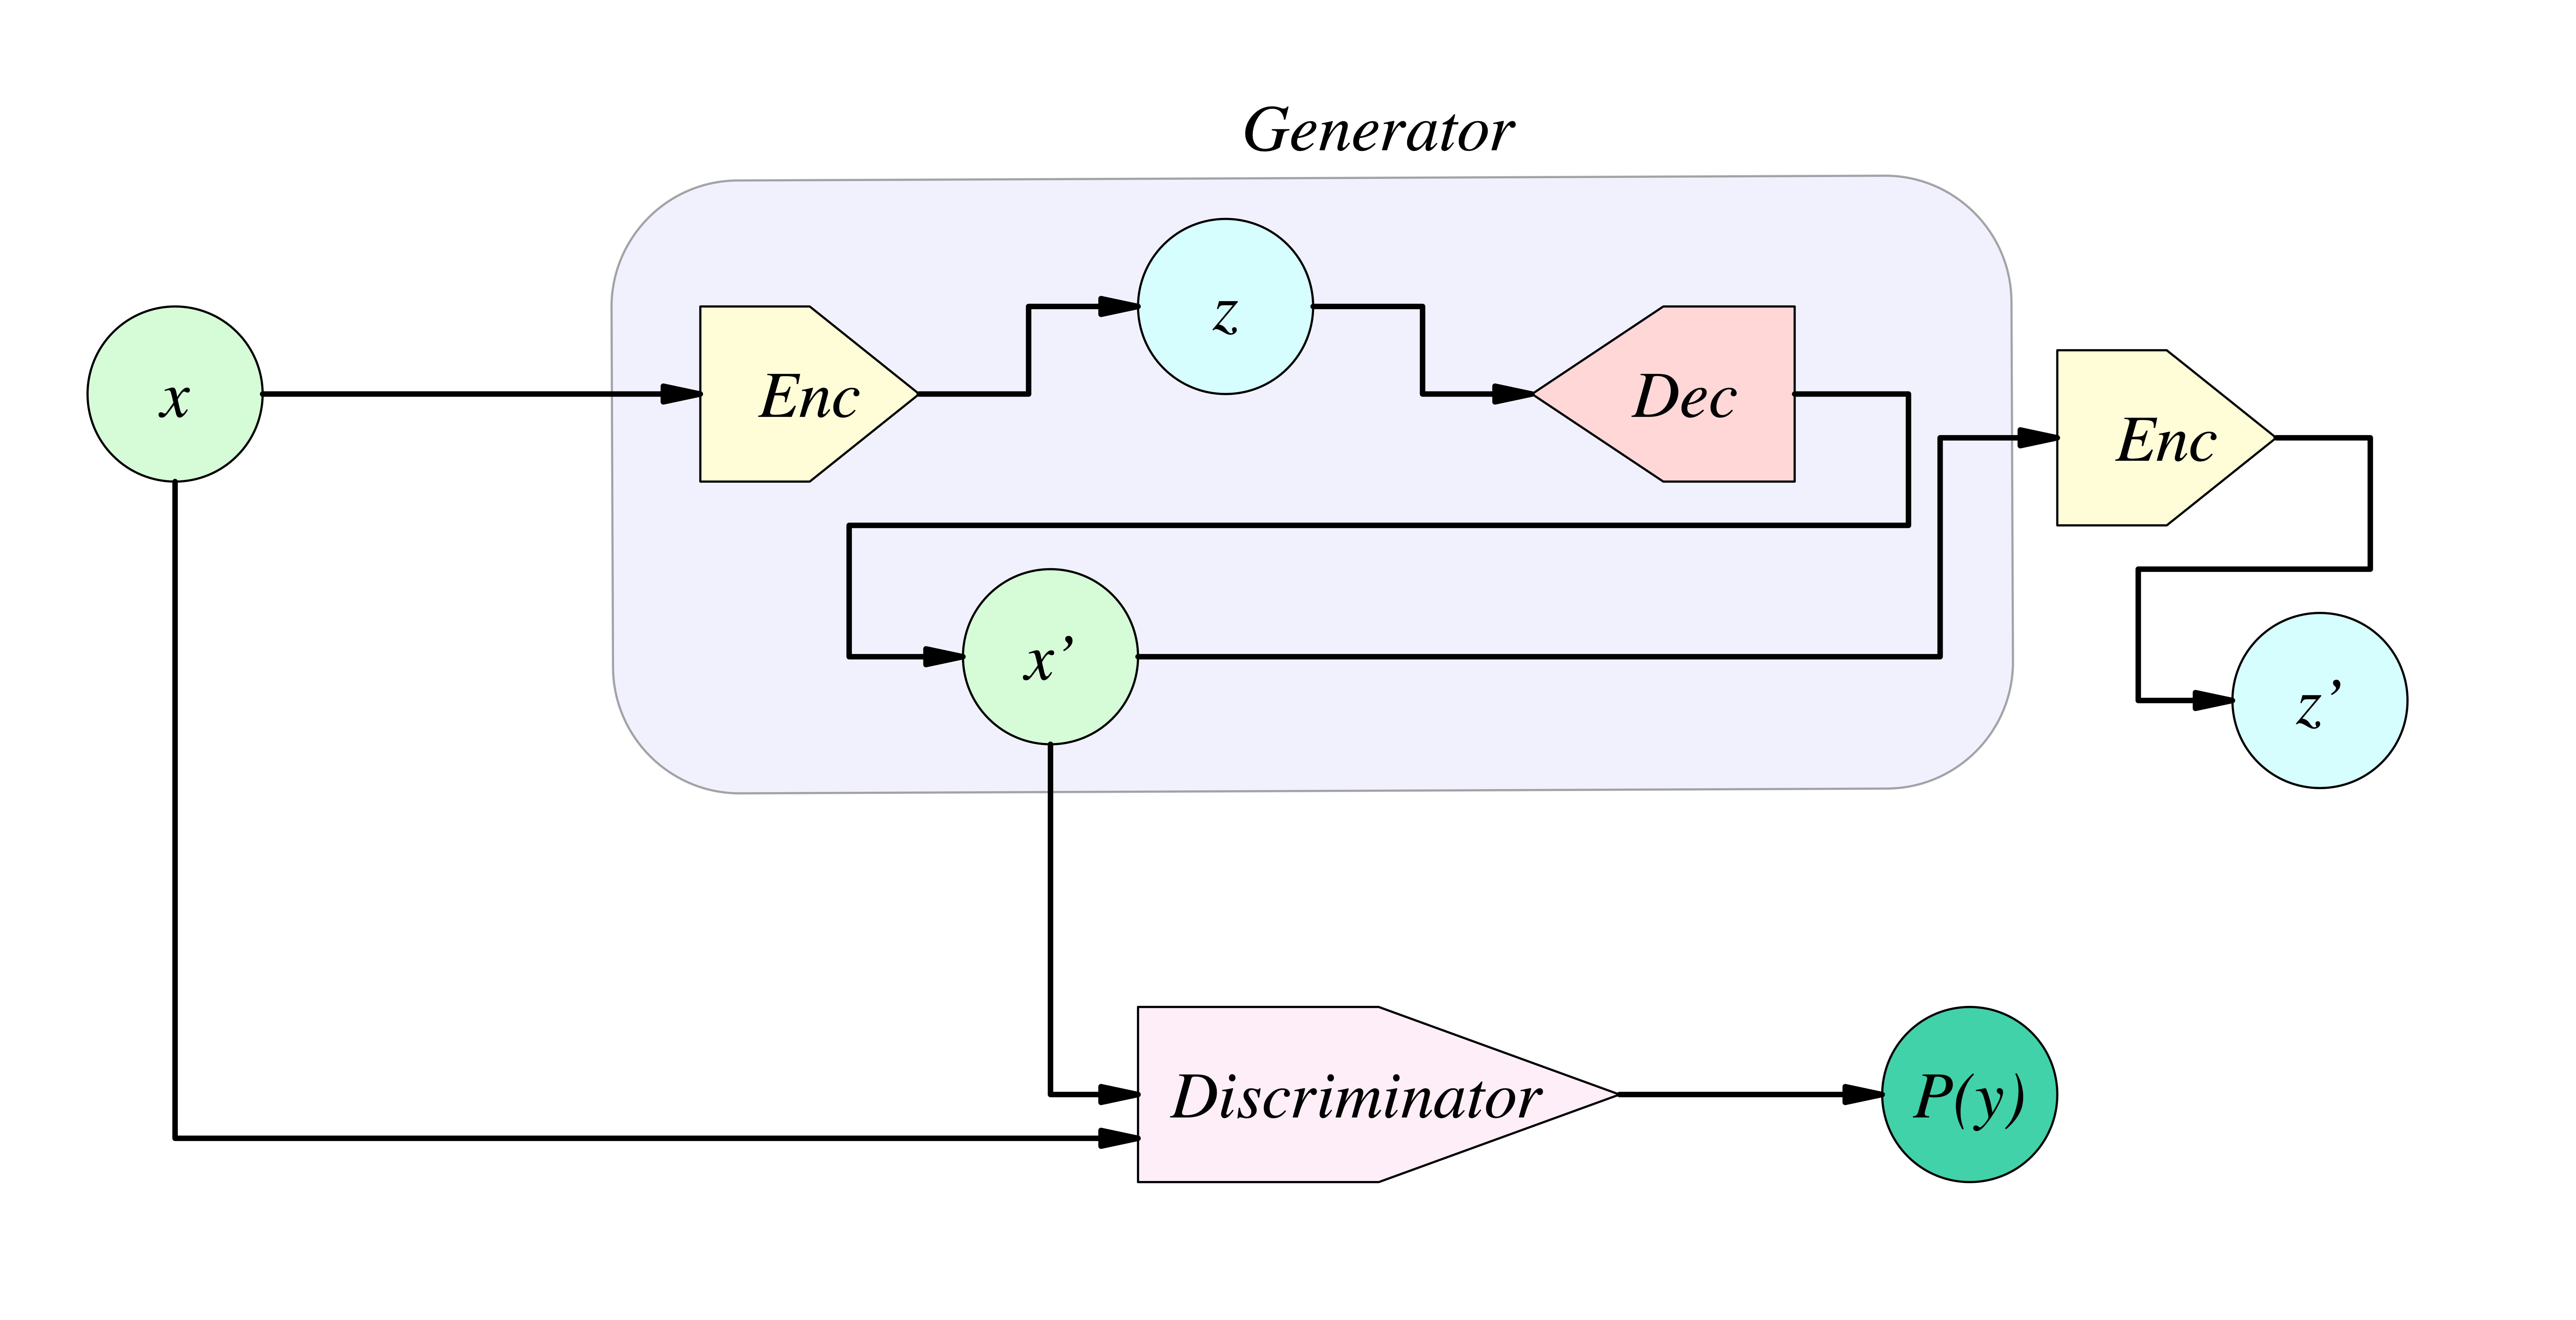
\includegraphics[width=.9\textwidth]{ganomaly}
    \caption{GANomaly architecture overview}
    \label{fig:ganomaly_model}
\end{figure}

 With the use of the adversarial autoencoders, framework obtains a superior reconstruction ability
compared to the previous models. But in doing so, its generative sub-module decoder is not a true
generative component from the perspective of the generative adversarial networks. With the change of
the model architecture its training objective also changes. GANomaly framework uses adversarial
training scheme but its generator module loss is the combination of 3 separate loss functions. These
are:
\begin{itemize}
   \item Adversarial Loss
   \item Contextual Loss
   \item Encoder Loss 
\end{itemize} 

Adversarial loss represents the loss function component for the adversarial training of the
framework. Instead of maximizing the probability of discriminator's attaining generated image as
real, it has a loss function derived from the \cite{fm} that uses feature matching. The main purpose
of this type of loss function is to reduce the instability in the GAN training. Adversarial loss
depicted in equation \ref{eqn:ganomaly_adv} is the $\mathcal{L}_{2}$ distance of the feature
representation of the original and the generated image, respectively. \cite{Akay2018GANomalySA}
Feature layer is extracted from the activation layer before the output of the discriminator.  
\begin{equation}
    \label{eqn:ganomaly_adv}
    \mathcal{L}_{a d v}=\mathbb{E}_{x \sim p_{\mathbf{x}}}\left\|f(x)-\mathbb{E}_{x \sim p_{\mathbf{x}}} f\left(G(x) \|_{2}\right.\right. 
\end{equation}

Only adversarial loss does not help to optimize the generator towards reconstructing images similar
to the input data. To this end, contextual loss is also added to the generator loss function.
According to \cite{Isola2017ImagetoImageTW}, using $\mathcal{L}_1$ instead of $\mathcal{L}_2$
decreases the blurriness in the generated images, so the following contextual loss that measures the
distance between original image and the generated one is added to the to the total generator loss.
\begin{equation}
    \mathcal{L}_{c o n}=\mathbb{E}_{x \sim p_{\mathbf{X}}}\|x-G(x)\|_{1} 
\end{equation}

Additional encoder loss is also added to the generator to improve the encoding of the latent
representation of the reconstruction. This loss function aims to minimize the distance between the
encoded latent representation of the input image and the reconstruction. The Loss function is
depicted below.
\begin{equation}
    \mathcal{L}_{e n c}=\mathbb{E}_{x \sim p_{\mathbf{X}}}\left\|G_{E}(x)-E(G(x))\right\|_{2} 
\end{equation}

Overall, the objective loss function of the generator is defined in equation
\ref{eqn:ganomaly_oall} where the weight parameters $w_{adv}, w_{con} \text { and } w_{enc}$
are used to change the impact of individual losses.
\begin{equation}
    \label{eqn:ganomaly_oall}
    \mathcal{L}=w_{a d v} \mathcal{L}_{a d v}+w_{c o n} \mathcal{L}_{c o n}+w_{e n c} \mathcal{L}_{e n c} 
\end{equation}

GANomaly framework uses encoder loss function also as an anomaly score measure.  
\begin{equation}
\label{eqn:ganomaly_as}
    \mathcal{A}(\hat{x})=\left\|G_{E}(\hat{x})-E(G(\hat{x}))\right\|_{1}  
\end{equation}

Skip-GANomaly framework\cite{Akay2019SkipGANomalySC} is the continuation of the GANomaly architecture with changes mainly to the
generator network. As can be seen from figure \ref{fig:sganomaly_model}, encoder and decoder
networks inside the generator framework is connected using skip connections. 
\begin{figure}[h!]
	\centering
	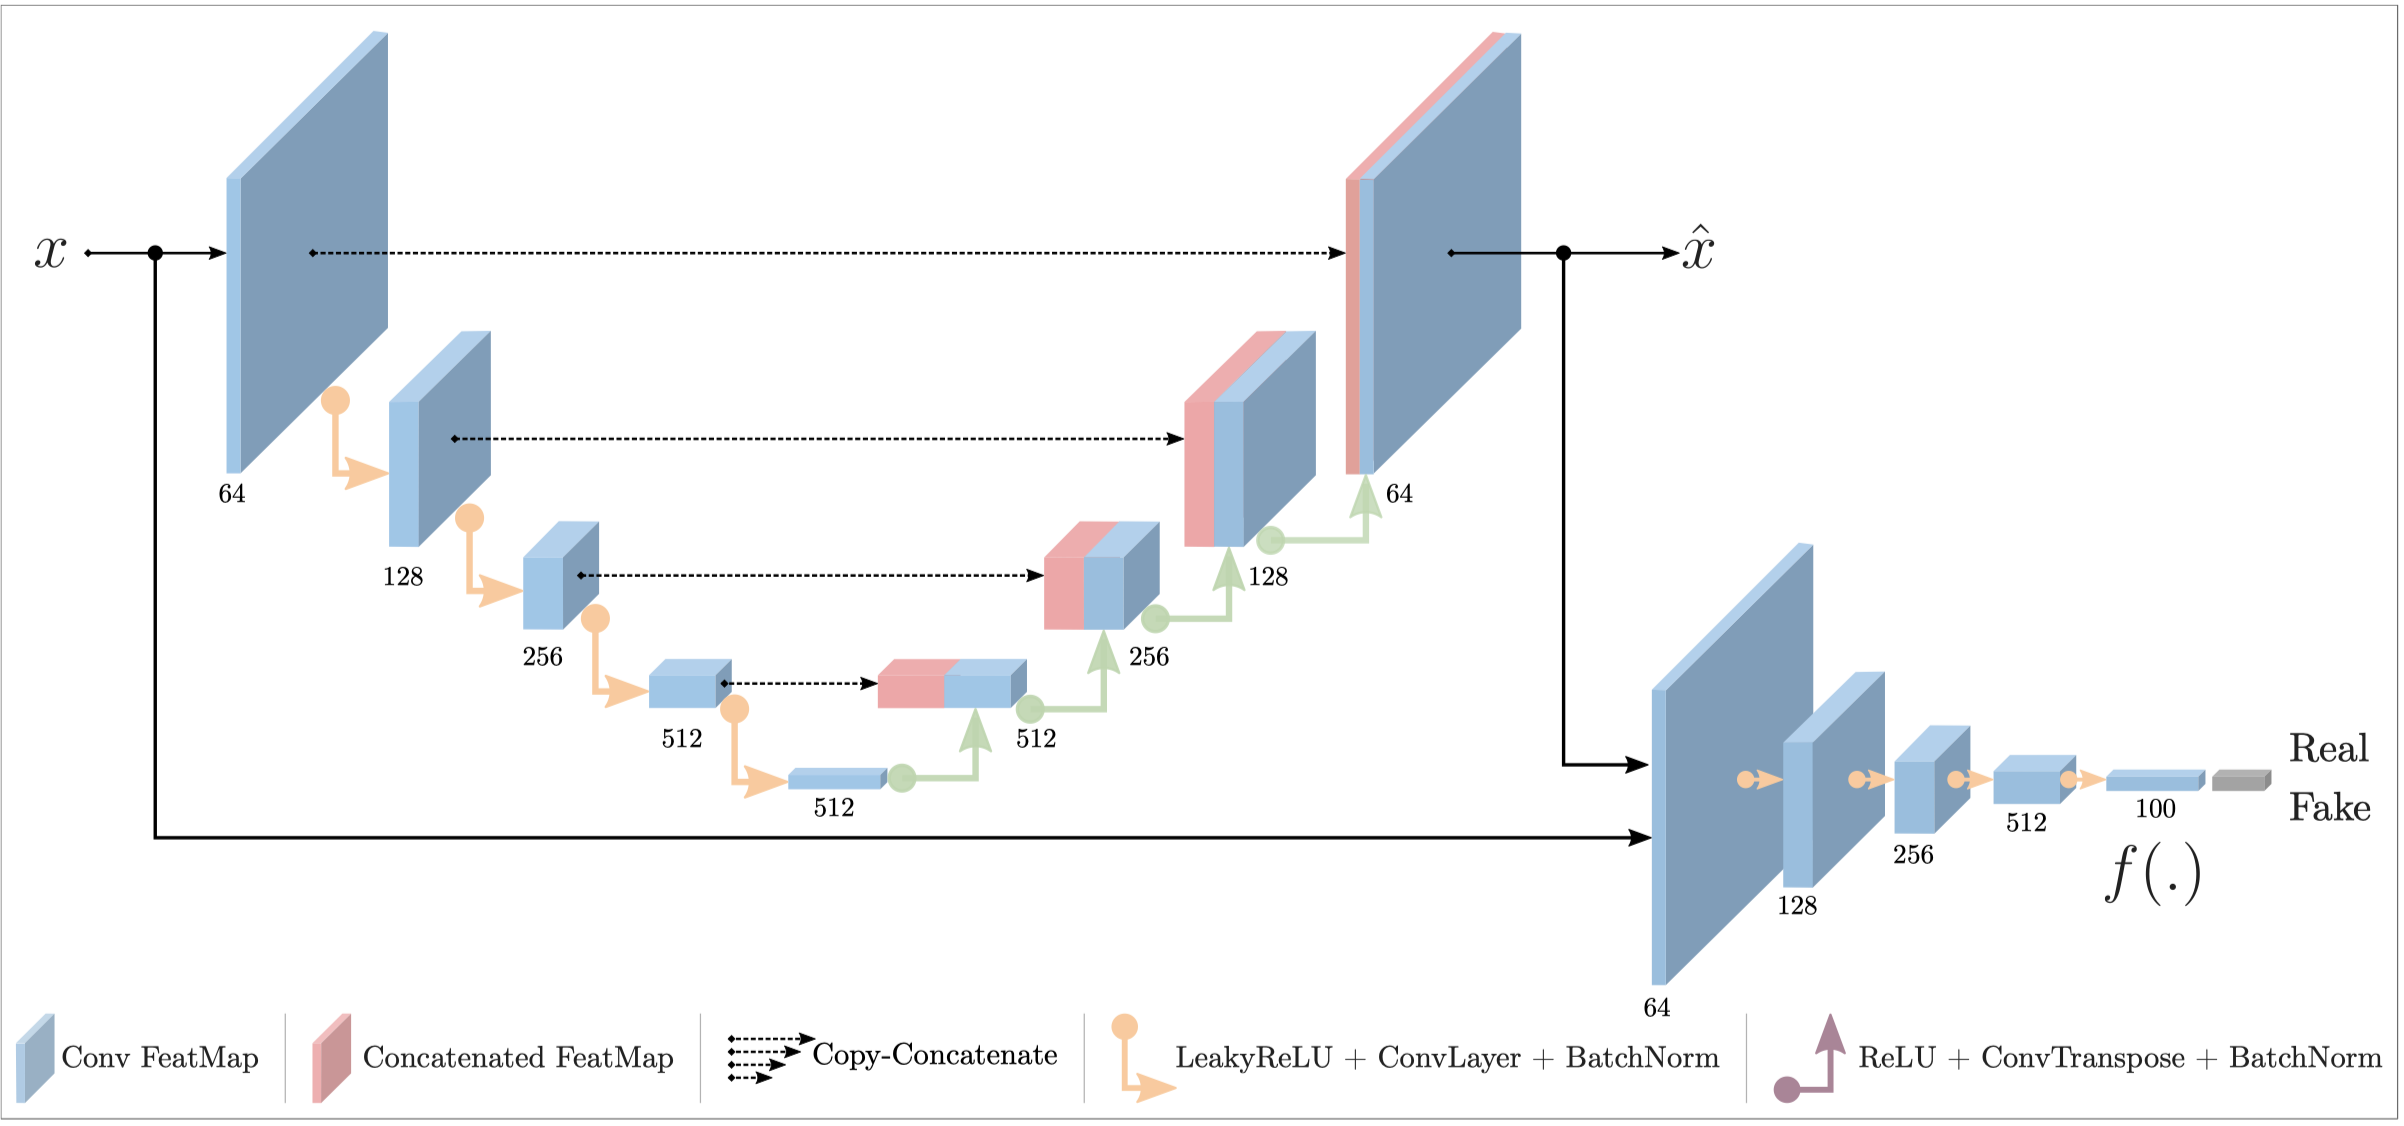
\includegraphics[width=.9\textwidth]{skip_ganomaly}
    \caption{Skip GANomaly architecture overview \cite{Akay2019SkipGANomalySC}}
    \label{fig:sganomaly_model}
\end{figure}

At each layer of the encoder, convolutional feature map is concatenated to the corresponding decoder
layer. Addition of skip connections provides a better reconstruction capability to the generator
than the GANomaly framework. \cite{Akay2018GANomalySA}. Generator objective function is built using
the same logic. Because of the exclusion of the secondary encoder network, the encoder loss is
obtained using the feature layer of the discriminator. 
\begin{equation}
    \mathcal{L}_{enc}=\underset{x \sim p_{x}}{\mathbb{E}}|f(x)-f(\hat{x})|_{2}  
\end{equation}

To find anomalies during the inference stage, Skip-GANomaly framework combines the encoder loss with
the use of contextual loss. 
\begin{equation}
	\label{eqn:sganomaly_as}
    \mathcal{A}(\dot{x})=\lambda R(\dot{x})+(1-\lambda) L(\dot{x})  
\end{equation}

$R(\dot{x})$ represents the contextual loss with the reconstruction term and $L(\dot{x})$ represents
the encoder loss with the latent representation term. Term $\lambda$ is used to adjust the impact of
the loss functions to the overall anomaly score.

Both GANomaly and Skip-GANomaly uses adversarial encoder architecture in their generator networks
and therefore have superior reconstruction capabilities compared to the previous 3 framework. The
primal problem with their architecture is that they don't adapt the true distribution of the input
data. They learn the underlying latent representation well to reconstruct the input and detect
anomalies. However their generator network represents the scenario where  generator has learnt the
input data distribution fairly well. In order to improve the results of a GAN based anomaly
detection framework, insights gained from these 2 networks are significantly important. Their
contribution to the improved framework and their performance analysis regards to other models will
be explored in chapters \ref{chap:arim} and \ref{chap:expres} respectively. 
\endgroup

% %-------------------------------------------------------------------------------
\chapter{Latest Developments}
\label{chap:latdel}
%!TEX root = ../2019_7_Ozgumus_Semsi_Yigit.tex

\begingroup

\begingroup
{
	\color{Green}

This chapter presents the developments in the field of anomaly detection and generative adversarial
networks. Although the models introduced in Chapter \ref{chap:sota} deliver certain level of
performance, potential improvements are still a possibility. These improvements are related to both
adversarial training of the generator and discriminator networks and applying different training strategy to 
stabilize the training of encoder network presented in the overall model. Section \ref{sec:fanogan} and 
\ref{sec:ebgan} presents some of these improvements that are later adopted by our model. Their contribution
to solve the disadvantages we observed in the previous model will be discussed. 

\section{F-AnoGAN }
\label{sec:fanogan}

AnoGAN \cite{Schlegl2017UnsupervisedAD} is considered as the first moel that uses generative
adversarial networks for an anomaly detection task. The main problems with this model, are the
stabilization issues of the adversarial training, and inference stage of the model that
maps from the latent representation to the input data distribution
as the inverse mapping of generator network. Model used back propagation to approximate the latent
representation for every query image to compute the anomaly score which resulted a very poor
performance in terms of the computation time. This was the main disadvantage of the model
because it is very challenging to integrate into a real life application with an implausible
inference time. F-AnoGAN (Fast AnoGAN ) model \cite{pub.1111824956} aims to eliminate the inference computation time 
problem by implementing an encoder network with a new training strategy. It also uses a new objective function for the adversarial
training to further stabilize the generator discriminator performance. In the rest of this section,
F-AnoGAN model, its training strategies and anomaly detection methods will be discussed.

Architecture of F-AnoGAN is very similar to the BiGAN \cite{Donahue2017AdversarialFL}
model. It consists of a generator discriminator for the adversarial learning and an encoder
network to learn the inverse mapping from latent representation to the input image data.
\begin{figure}[h!]
	\centering
	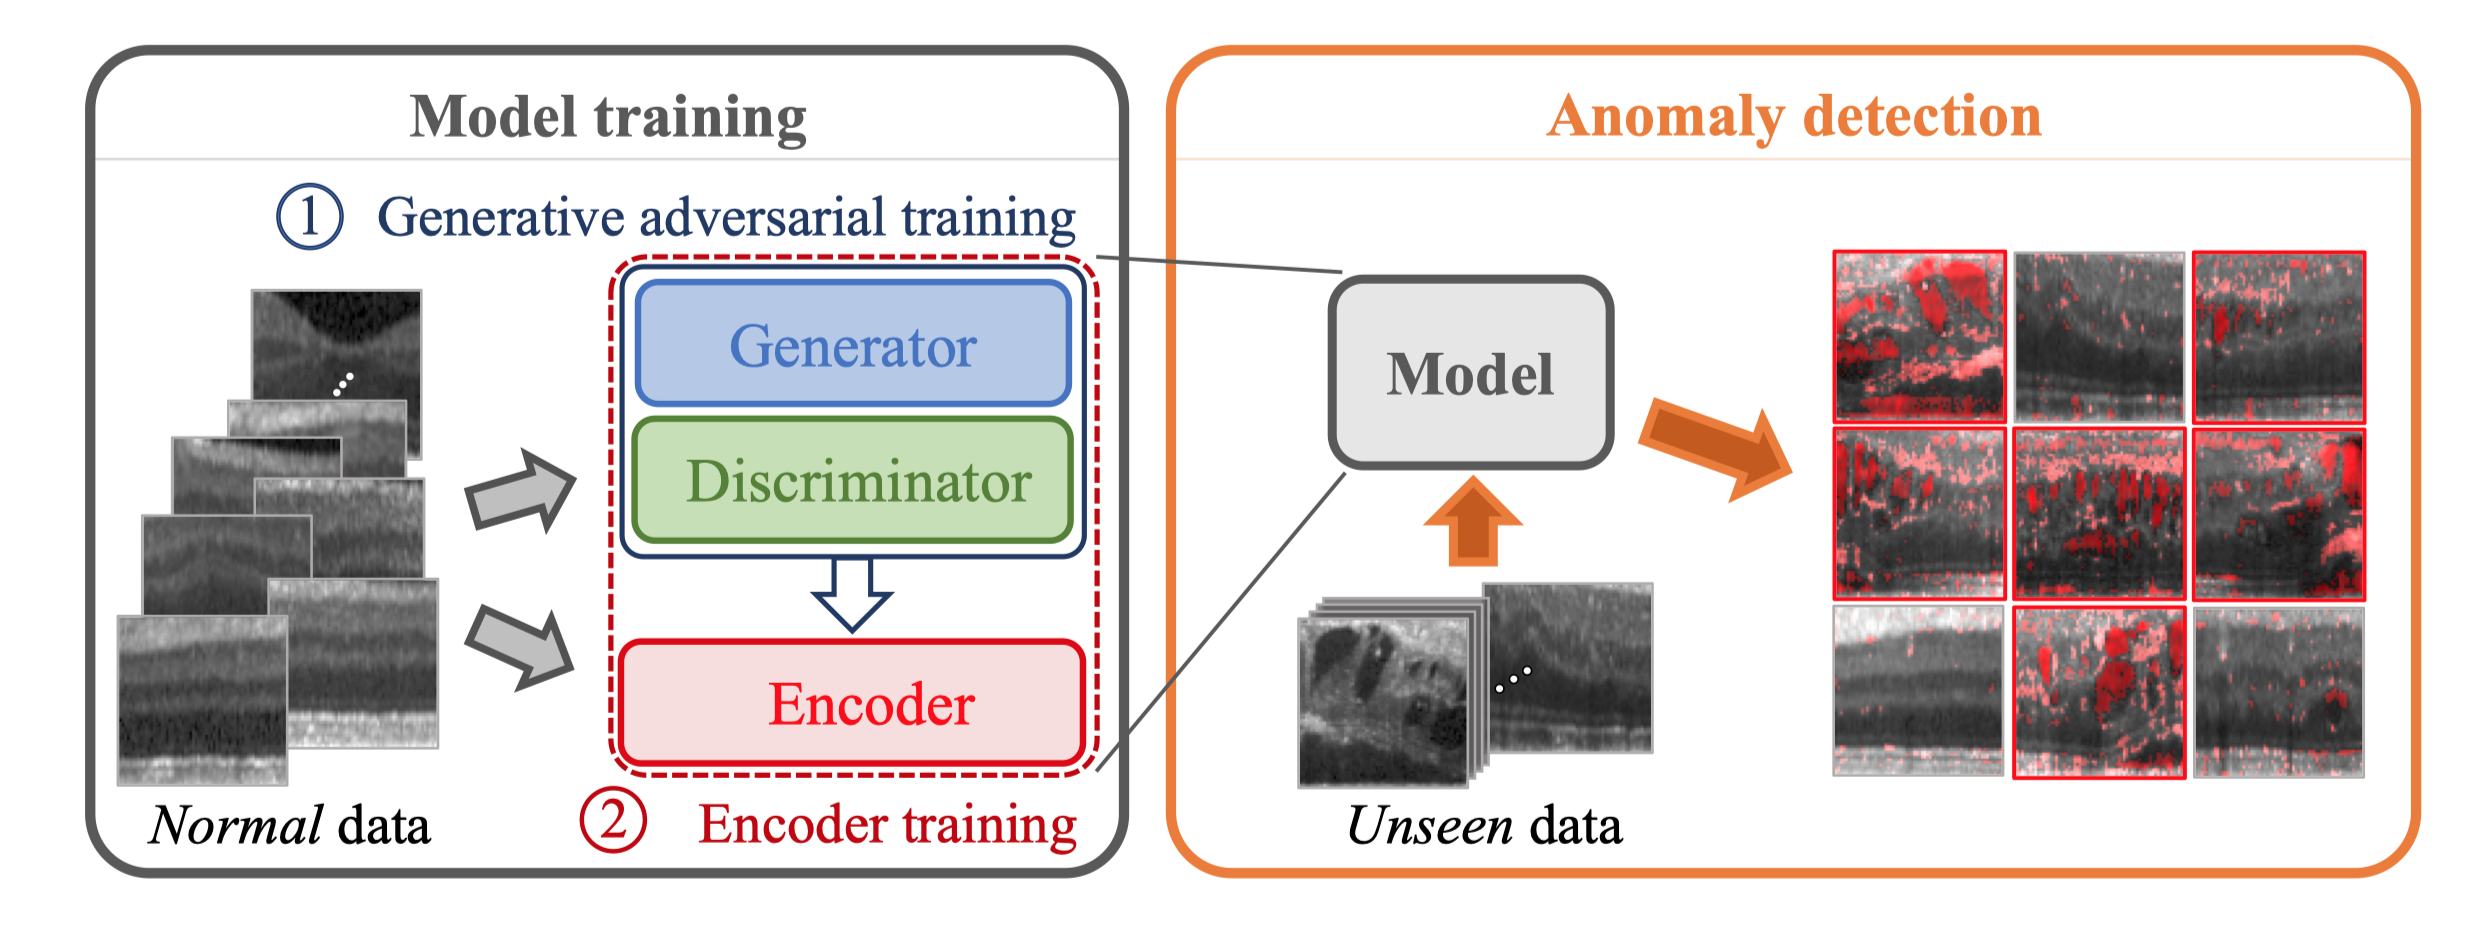
\includegraphics[width=.9\textwidth]{fanogan_framework}
	\caption{F-AnoGAN Model Overview \cite{pub.1111824956}}
	\label{fig:fanogan_network}
\end{figure}

The first improvement is the change of training style of the whole model. In BiGAN approach,
encoder and generator networks are trained simultaneously to fool the discriminator. Hence discriminator is
modified to classify the pairs of noise (latent representation) and images instead of the single
image approach used in the GAN. It tries to distinguish samples from a joint
distribution which explained in Section \ref{sec:bigan}. Including encoder to the adversarial setup
also introduces instability issues which ALAD model \cite{DBLP:journals/corr/abs-1812-02288}
tried to mitigate with additional discriminators that approximate conditional entropy. (see Section
\ref{sec:alad_alice}). F-AnoGAN model addresses this issue by separating the training of
encoder network $E$ from the generator discriminator networks. New model can be seen in Figure
\ref{fig:fanogan_training}. 
\begin{figure}[h!]
	\centering
	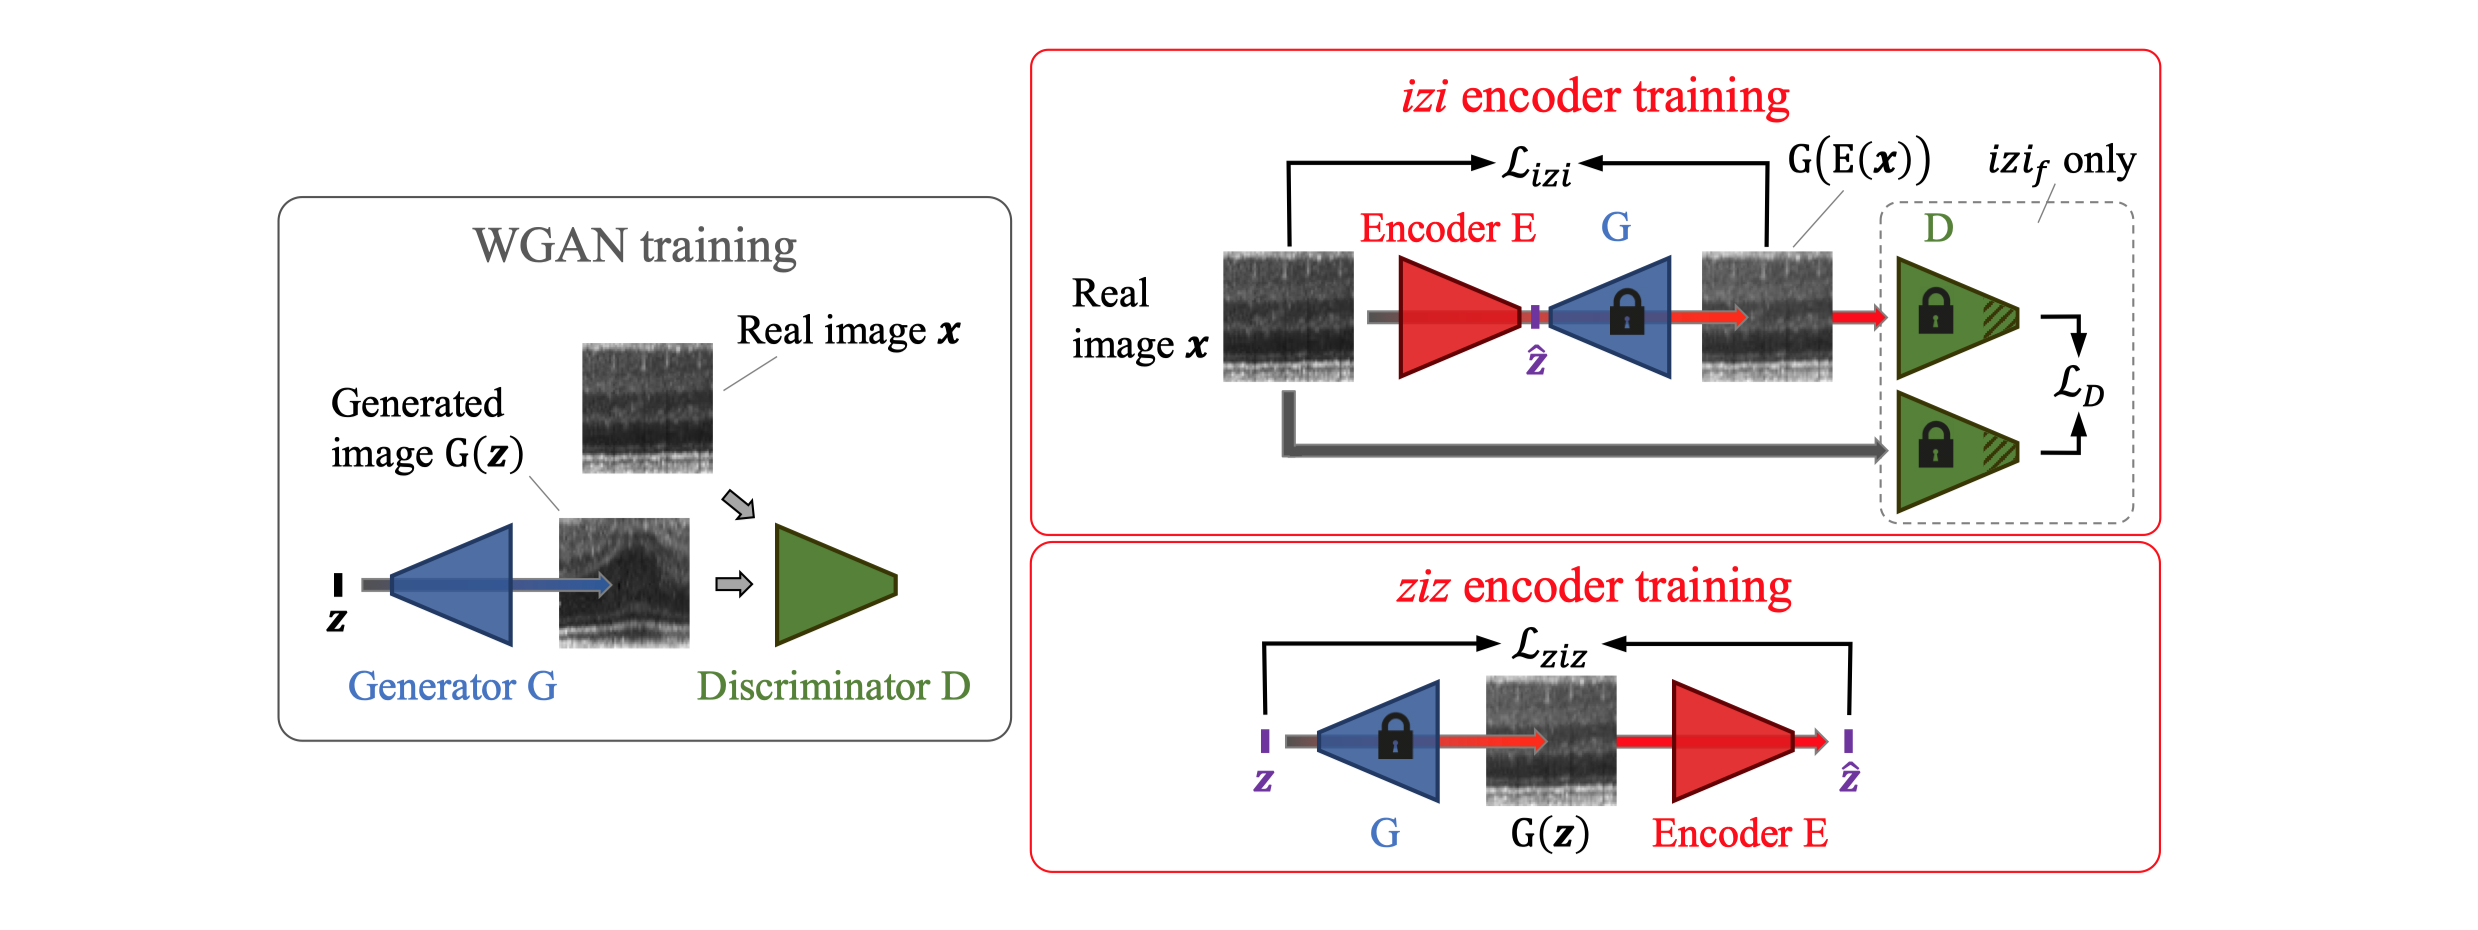
\includegraphics[width=.9\textwidth]{fanogan_training}
	\caption{F-AnoGAN Training Strategies \cite{pub.1111824956}}
	\label{fig:fanogan_training}
\end{figure}

This new training scheme comprises of two stages. In the first stage GAN model is trained.
Objective function for the adversarial training is also replaced with the Wasserstein GAN's
objective function \cite{Arjovsky2017WassersteinG} 
% appendix explanation ?
although training of the GAN can be performed with other training methods (including the
original GAN) according to the \cite{pub.1111824956}.

In the second stage, encoder network is trained using generator and discriminator networks with fixed
weights. Two separate pipelines are used to measure the performance of the encoder network. These are $IZI$
(image-noise-image) and $ZIZ$ (noise-image-noise) respectively. 

\textbf{IZI Encoder Training}

$IZI$ method follows the standard autoencoder network architecture. Generator network with fixed
weights acts as a decoder network. During the training, same image dataset used in the first stage
for training GAN is mapped to a latent space $z$ by a trainable encoder and then reconstructed
using the fixed generator network. Training objective for this setup is to minimize MSE (Mean
Squared Error) based reconstruction error of the input image $x$ and the reconstructed image
$G(E(x))$. 
\begin{equation}
	\mathcal{L}_{i z i}(\mathbf{x})=\frac{1}{n}\|\mathbf{x}-G(E(\mathbf{x}))\|^{2}
\end{equation}
where $n$ is the total dimension size of the data.
This approach has an important drawback regarding to latent representation. Since the distribution
of the latent representation of the input image is not known, the encoder is trained only using a
form of contextual loss which enforce the similarity only in the image space. Without the
sufficient information about the latent space, encoder may map images to a representations such
that the reconstructions are not convincing enough for the discriminator to evaluate as real
\cite{pub.1111824956}. Therefore model suggests including a latent space based loss
function derived from the feature layer of the discriminator network to guide the encoder network 
training. Improved $IZI_{f}$ training objective is defined below.
\begin{equation}
	\mathcal{L}_{i z i_{f}}(\mathbf{x})=\frac{1}{n} \cdot\|\mathbf{x}-G(E(\mathbf{x}))\|^{2}+\frac{\kappa}{n_{d}} \cdot\|f(\mathbf{x})-f(G(E(\mathbf{x})))\|^{2}
\end{equation}

where the $f(\cdot)$ represents the feature layer of the discriminator as an additional statistics, $n_{d}$ is
the dimensionality of the intermediate feature representation $f$ and $\kappa$ denotes the weighting
factor for the inclusion of the discriminator guidance.

\textbf{ZIZ Encoder Training}

This method reverses pipeline created on $IZI$ training and forms a decoder
encoder architecture. A random sampled noise from the latent $z$ space is mapped to the image space using the
fixed generator and then generated sample is encoded using the trainable encoder network. Loss
for the training objective is defined as the MSE based reconstruction of the noise which depicted in Equation
\ref{eqn:ziz} where $d$ is the total dimension of the latent representation.
\begin{equation}
\label{eqn:ziz}
	\mathcal{L}_{z i z}(\mathbf{z})=\frac{1}{d}\|\mathbf{z}-E(G(\mathbf{z}))\|^{2}
\end{equation}

Main shortcoming of this approach is that even though the encoder network is trained with a loss that will
enforce a similarity in latent space, encoder sees only images that are generated by the generator network.
It doesn't see any image samples from the training dataset which affects the contextual similarity
of the reconstruction of learned latent space distribution. 

\begin{figure}[h!] 
	\subfloat[Anomaly Score computation scheme for izi and $izi_f$ method]{
		\begin{minipage}[c][0.5\width]{0.5\textwidth}
			\centering
			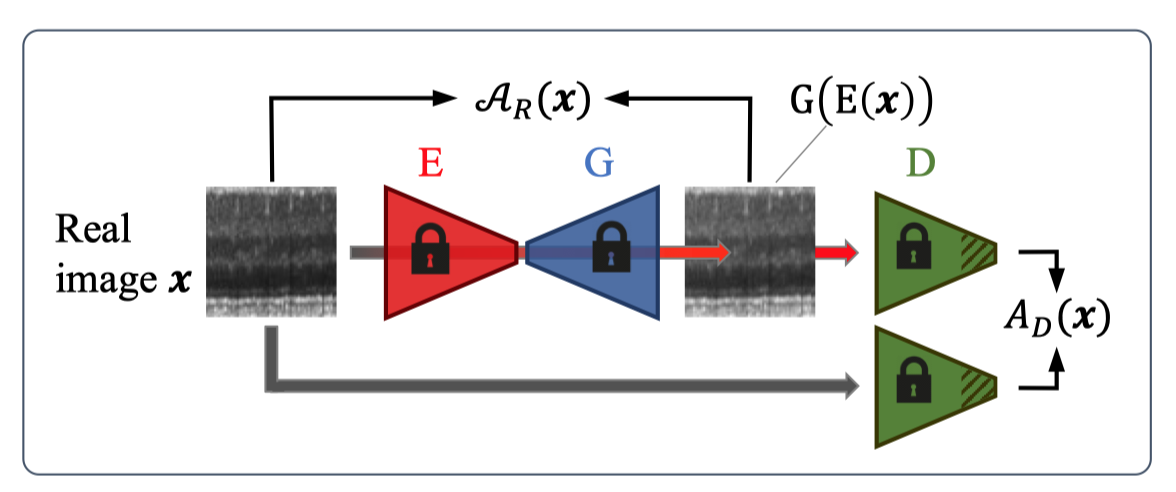
\includegraphics[width=1\textwidth]{fanogan_anomaly_1}
	\end{minipage}}
	\hspace*{\fill}%
	\subfloat[Anomaly Score computation scheme for ziz architecture]{
		\begin{minipage}[c][0.5\width]{0.5\textwidth}
			\centering
			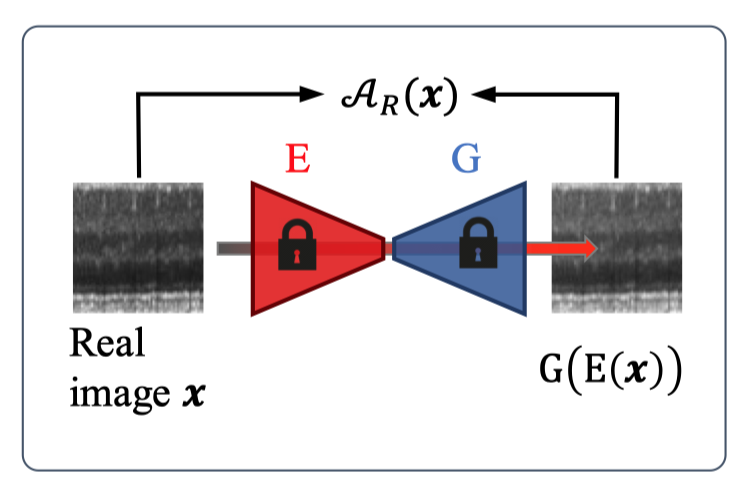
\includegraphics[width=0.6\textwidth]{fanogan_anomaly_2}
	\end{minipage}}
	\caption{Anomaly Score computations for both training methods \cite{pub.1111824956}}
	\label{fig:fanogan_anomaly_score}
\end{figure}

To calculate the anomaly score for inference, deviation of the query images from their
reconstructions are quantified. Figure \ref{fig:fanogan_anomaly_score} represents the anomaly score
computations for both training methods.

 $IZI_f$ method uses the same loss functions for the computation of the anomaly score. Anomaly score
 for image $x$ is defined as:
\begin{align}
	\mathcal{A}(\mathbf{x})&=\mathcal{A}_{R}(\mathbf{x})+\kappa \cdot \mathcal{A}_{D}(\mathbf{x}) \\[5pt]
	\mathcal{A}_{R}(\mathbf{x})&=\frac{1}{n} \cdot\|\mathbf{x}-G(E(\mathbf{x}))\|^{2} \\[5pt]
	\mathcal{A}_{D}(\mathbf{x})&=\frac{1}{n_{d}} \cdot\|f(\mathbf{x})-f(G(E(\mathbf{x})))\|^{2}
\end{align}

where $\mathcal{A}_R (x)$ represents the reconstruction based loss and $\mathcal{A}_{D} (x)$ represents the 
latent loss that uses feature layer of discriminator network.
For $IZI$ and $ZIZ$ method, the computation of the anomaly score reduces down to
$\mathcal{A}_{R}(\mathbf{x})$ function only. Both training methods yields a similar anomaly score
computation for the anomalous samples. Since the models are trained with a dataset that doesn't
contain any anomalies, query images that have anomalous regions results in poorer reconstruction
hence a higher anomaly score while the normal images produce a more similar reconstructions to the
original sample.
 
Significance of this model is that it separates the training of encoder network from the
adversarial setting of the GAN's while preserving the inverse mapping functionality for the
inference and keeping the inference time of the model relatively short. Chapter 
\ref{chap:arim} will explain its contribution to the proposed model.

} %%%%%%%%% CONTROL POINT
%%%%%%%%%%%%%%%%%%%%%%%%%%
\section{Energy Based Generative Adversarial Networks}
\label{sec:ebgan}

Training a GAN perhaps the most sensitive part of working with them. There has been an
extensive amount of research to improve the stabilization of the adversarial training or perhaps
offer a new methodology. \cite{fm} and \cite{methods} offer number modifications to the original
adversarial training setup to improve the generation performance ,increase the stabilization and
prevent issues such as mode collapse\footnotemark. \cite{Arjovsky2017WassersteinG} and
\cite{Gulrajani2017ImprovedTO} offers a new method to compute the loss and ways to stabilize it.
Mainly because of its adversarial setting, training of GANs will always be a topic of
interest. Energy based generative adversarial networks \cite{Zhao2016EnergybasedGA} offers a new
training method by redefining the loss functions and the functionality of the discriminator network.
This section will introduce the architecture and how it works.

\footnotetext{Mode collapse is the scenerio where generator learns enough information to fool the 
	discriminator very early. It finds a generation that fools the discriminator and does not learn 
	anything else from the discriminator. Because of that all the generated samples from the generator 
	look the same, defeating the purpose of generating from the distribution of the data.\cite{methods}}

Energy based models measures the current state of the model by assigning a scalar predefined energy
as a degree of compatibility \cite{LeCun06atutorial}. Training energy based models consists of
mapping low energy outputs to the samples with the "correct" class, and mapping higher energy
outputs to the "incorrect" class. From the perspective of GANs, EBGAN model is trained to ouput
lower energy for the real data, while the generated data (fake images) outputs a higher energy. The
model architecture can be seen in figure \ref{fig:ebgan_model}.

\begin{figure}[h!]
	\centering
	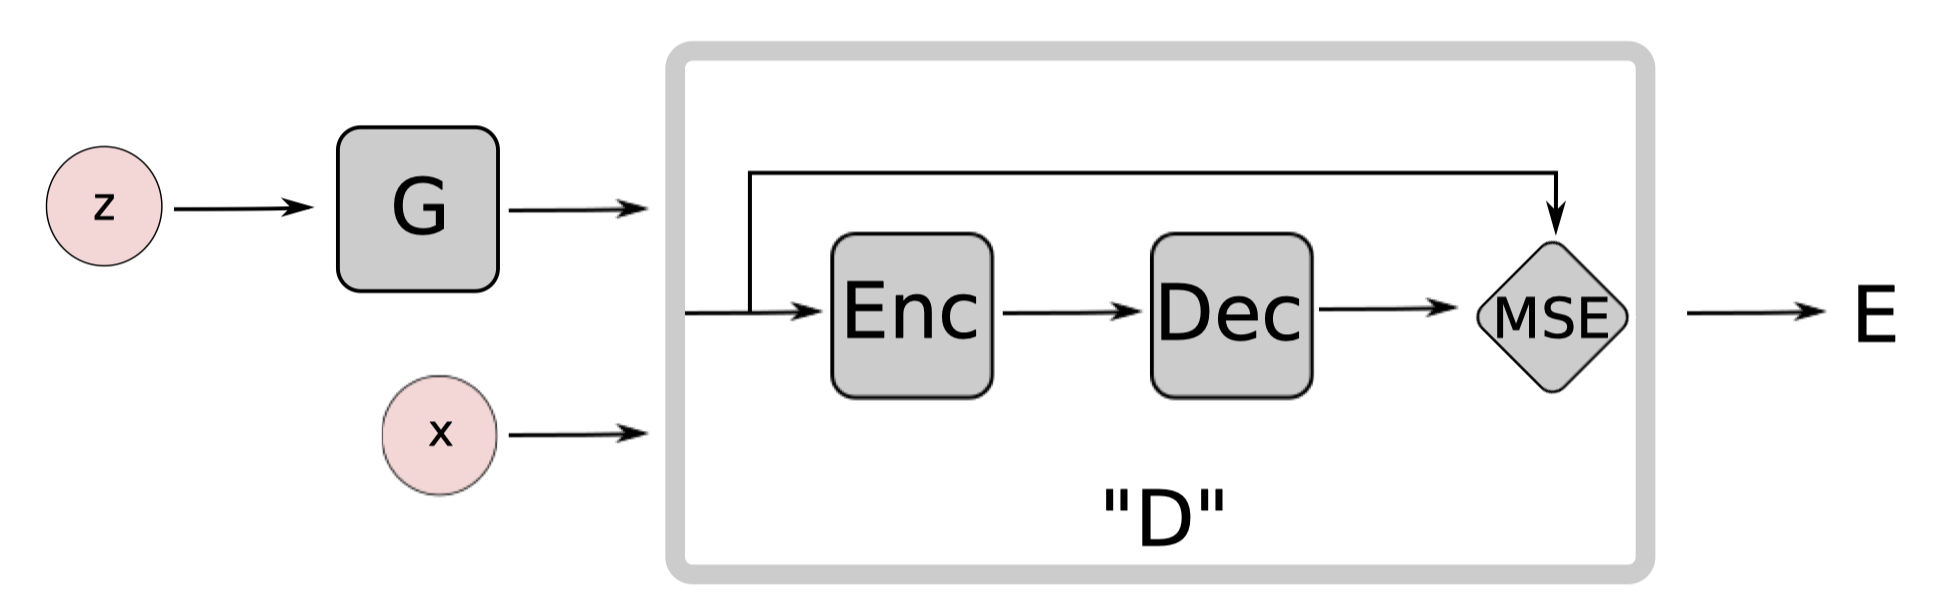
\includegraphics[width=1.0\textwidth]{ebgan_model}
	\caption{EBGAN Model Structure \cite{Zhao2016EnergybasedGA}}
	\label{fig:ebgan_model}
\end{figure}

The main structural difference of this framework from the other ones is that discriminator is
defined as an auto encoder network to provide the reconstruction of the inputs. The energy value
function is defined as the margin loss of the input and the reconstructed sample
\cite{Zhao2016EnergybasedGA} as a reconstruction error. 

Formally a margin is used to create an energy gap between the correct output and the incorrect
output. For data sample $x$, and a generated sample $G(z)$ with $z$ being sampled from a known
distribution $p_z$, The discriminator loss $\mathcal{L}_{D}$ and the generator loss
$\mathcal{L}_{G}$ are formally defined in equation \ref{eqn:ebgan_formal}.

\begin{equation}
\label{eqn:ebgan_formal}
\begin{aligned}D(x)&=\|\operatorname{Dec}(E n c(x))-x\|\\ \mathcal{L}_{D}(x, z) &=D(x)+[m-D(G(z))]^{+} \\ \mathcal{L}_{G}(z) &=D(G(z)) \end{aligned}
\end{equation}

where $D(x)$ is the reconstuction loss and  $[\cdot]^{+}=\max (0, \cdot)$. Minimizing
$\mathcal{L}_{G}$ with respect to the generator is similar to maximizing the second term of the
$\mathcal{L}_{D}$. Instead of calculating the probability of the input being real or fake,
discriminator is responsible for attaining the correct amount of energy to the input images. 

Using autoencoder network as a discriminator brings additional advantages to the training setting.
Rather than using a single target information to train the model, reconstruction based output offers
a more diverse targets for the discriminator \cite{Zhao2016EnergybasedGA}. One of the reasons that causes
stabilization issues in the adversarial training is that discriminator might provide gradients not
useful enough for generator to improve the quality of the generated samples. Having a reconstruction
loss output might provide a better gradient in terms of different directions as opposed to binary
logistic loss\cite{Zhao2016EnergybasedGA}. Another advantage is that even though they are trained with an adversarial setting,
autoencoder networks might prove useful to learn the underlying energy manifold of the data without
supervision or negative examples when they are trained using a proper regularization constraint.
This means that in this setting generated samples and input data are both used to model the
underlying energy manifold of the data. 

EBGAN argues that, the discriminator network is regularized by exposing generated samples
from the generator  which it should output higher reconstruction energies
\cite{Zhao2016EnergybasedGA}. The benefit of this regularization is that instead of a hand crafted
predefined one, the regularization term can also be trained along with the discriminator.
Adversarial training allows a direct connection between learning the energy function and producing
contradictive samples in that regard. 

EBGAN also adds additional penalty called pulling away term (PT) that run at a
representation level to prevent mode collapse depicted in equation \ref{eqn:ebgan_pt}.
\begin{equation}
\label{eqn:ebgan_pt}
	f_{P T}(S)=\frac{1}{N(N-1)} \sum_{i} \sum_{j \neq i}\left(\frac{S_{i}^{\top} S_{j}}{\left\|S_{i}\right\|\left\|S_{j}\right\|}\right)^{2}
\end{equation}

 $S$ is the feature output from the encoder for generated images. Pulling-away term measures the
 cosine similarity among all generated images features $S$ in a minibatch. If the mode collapses,
 the feature vectors will thereupon be similar, i.e. the angles are close to zero and the cosine
 will max-out. Therefore, it will add a high penalty if there are too similar.
 \cite{Zhao2016EnergybasedGA}
 
 EBGAN offers a more flexible approach to train the discriminator and generator network. 
 Transition from convolutional based discriminator to autoencoder network also provides a potential inclusion 
 for the computation of the anomaly score. Its impact on the proposed model will be discussed in the next chapter. 

\endgroup

%-------------------------------------------------------------------------------
\chapter{Architectural Improvements}
\label{chap:arim}
%!TEX root = ../2019_7_Ozgumus_Semsi_Yigit.tex

\begingroup

This chapter presents the modifications applied to aforementioned approaches to improve the
performance of the anomaly detection. All the discussed models measures its performance metric on
well known datasets, such as CIFAR-10 \cite{cifar10} and SVHN \cite{Netzer2011ReadingDI}. The
dataset used in this thesis presents additional challenges to this problem we aim to solve. The
first section will introduce its dataset to the reader and will give examples. Next section will
discuss the shortcomings of the previous approaches regarding the interpretation of the dataset and
detection of the existent anomalies. Sections \ref{sec:encebgan} and \ref{sec:sencebgan} will
explain the modified architecture and the significance of the changes.

\section{SEM Image Dataset}
\label{sec:sem}

Nanofibrous materials acquired increasingly significant demand from variety of fields in the
Industry. It constitutes a foundation material for a lot of products including areas in medicine,
filtration, sensors and manufacturing applications. \cite{carrera2016defect}. Despite the demand and
continuous research development towards its production, manufacturing nanofibrous materials is still
challenge for scaled of mass production. Several techniques for producing nanofibers have been
presented in the literature. \cite{carrera2016defect}. Electrospinning method is the focus of this
anomaly detection task. It produces a structure which consists of filaments woven in with randomized
geometric pattern. You can see one of the images of the material produced without any anomalies in
figure \ref{fig:data_norm}.

\begin{figure}[h!]
	\centering
	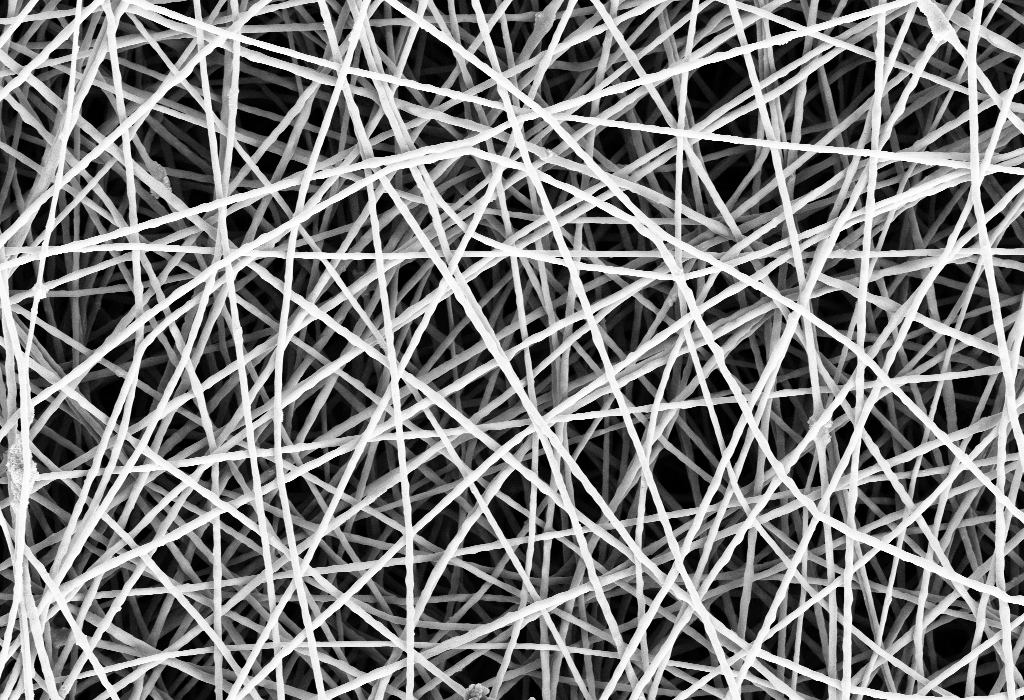
\includegraphics[width=0.75\textwidth]{dataset}
	\caption{Part of Training Dataset from the SEM Image Dataset \cite{sem}}
	\label{fig:data_norm}
\end{figure}

Dataset consists of 5 images with no anomalies and 40 sample images that have various types of
anomalous regions. To preserve computational efficiency without sacrifising from performance,
training dataset and testing dataset is sampled from SEM image dataset.
\begin{figure}[h!] \subfloat[Normal regions]{
		\begin{minipage}[c][0.8\width]{0.5\textwidth}
			\centering
			\fbox{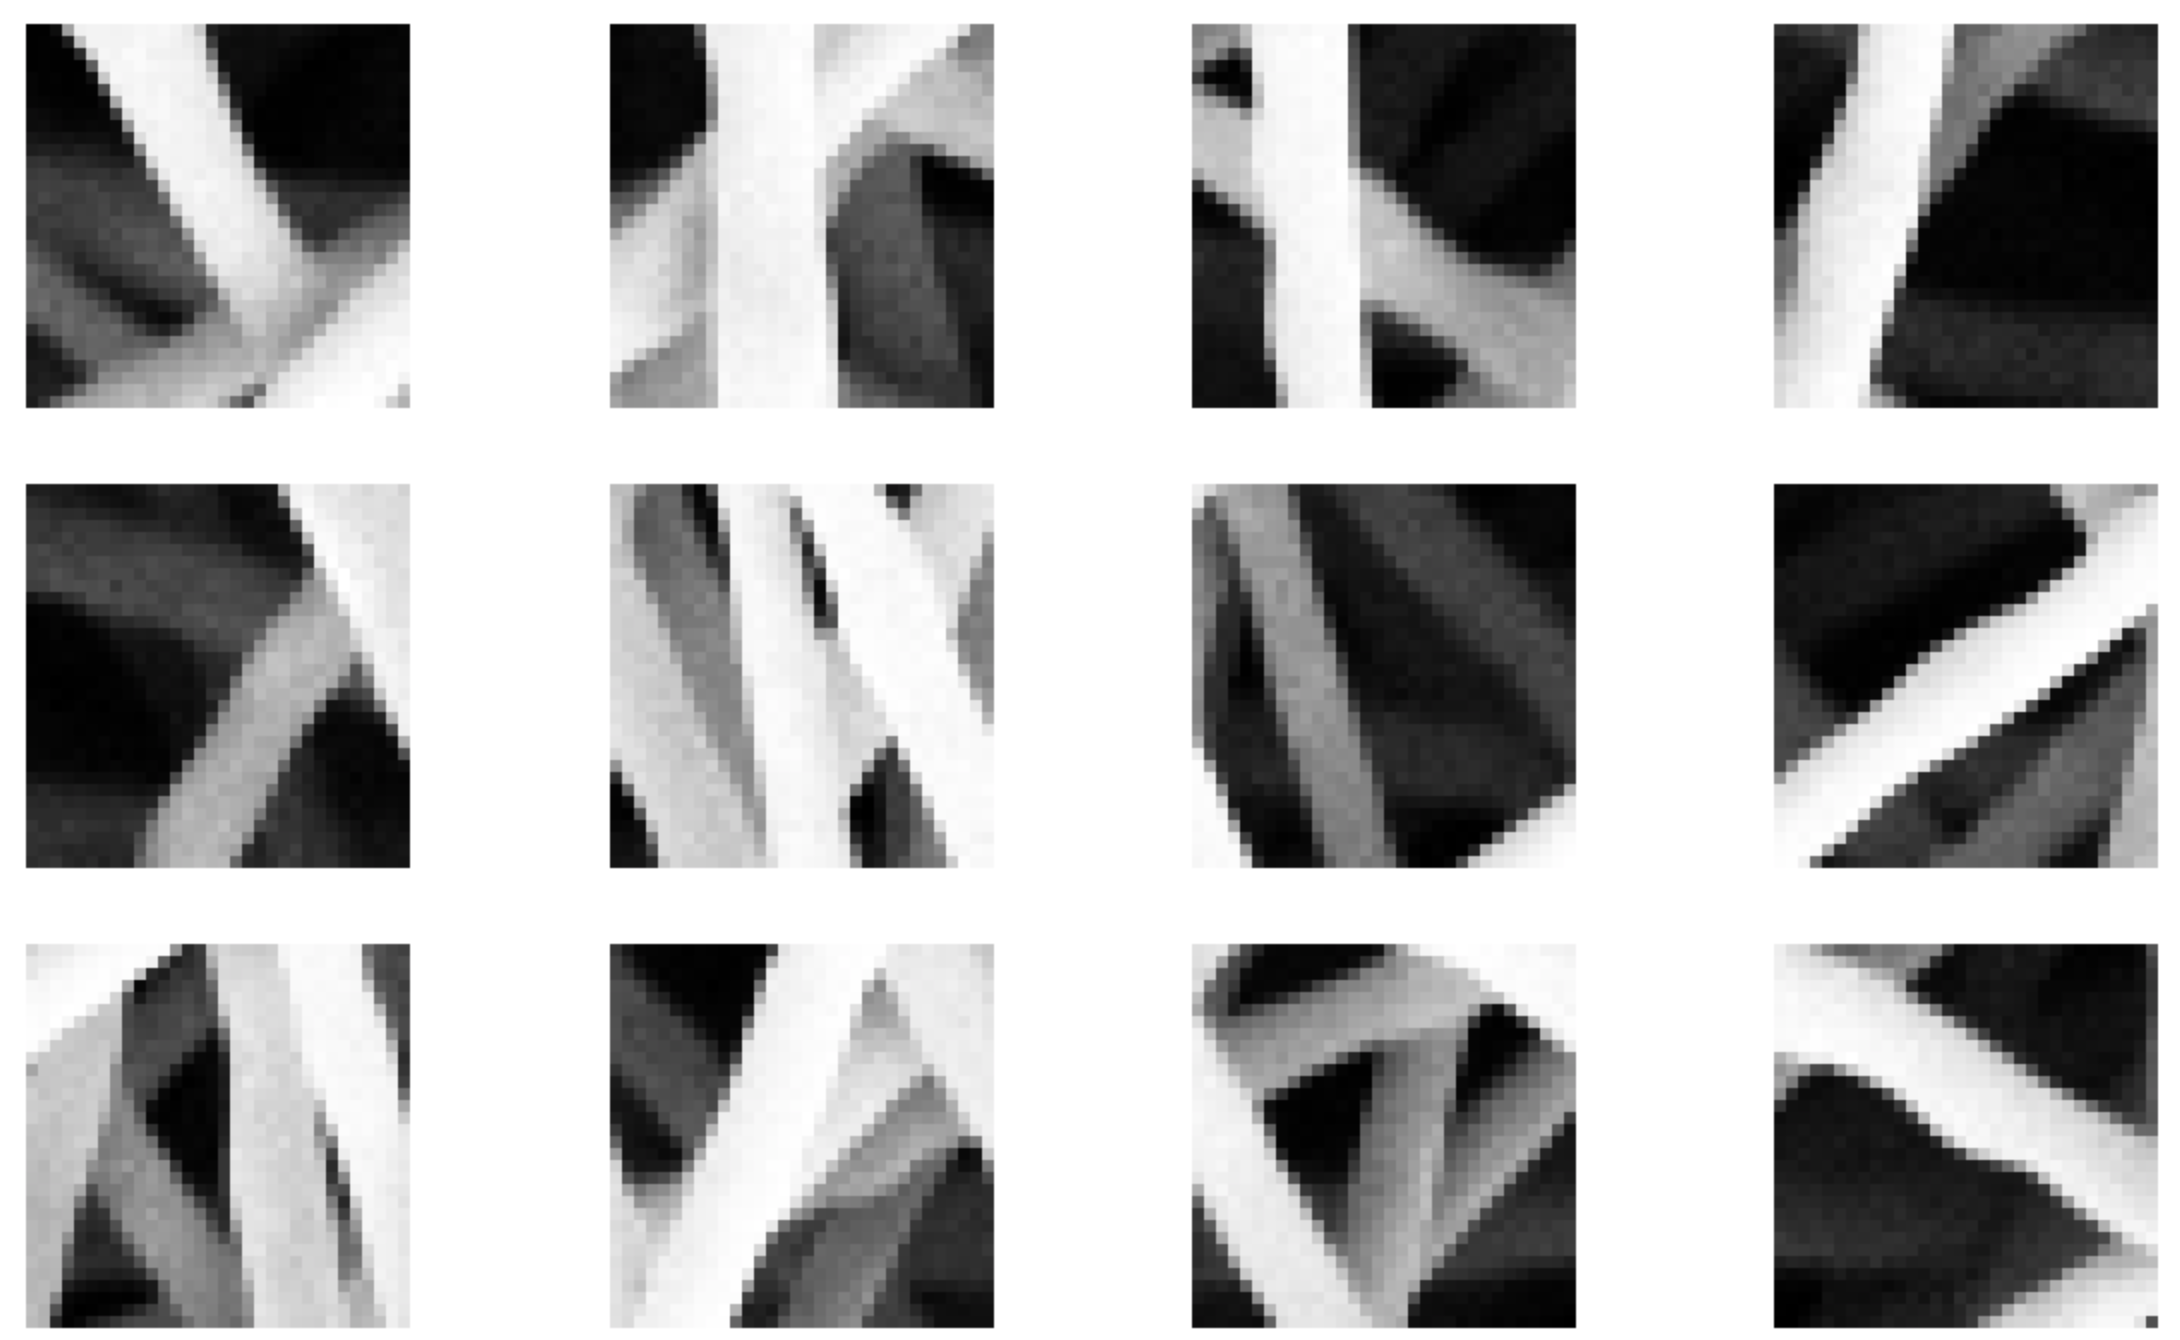
\includegraphics[width=1\textwidth]{sample_normal}}
			\label{fig:data_sample_normal}
	\end{minipage}}
	\hspace*{\fill} \subfloat[Anomalous regions]{
		\begin{minipage}[c][0.8\width]{0.5\textwidth}
			\centering
			\fbox{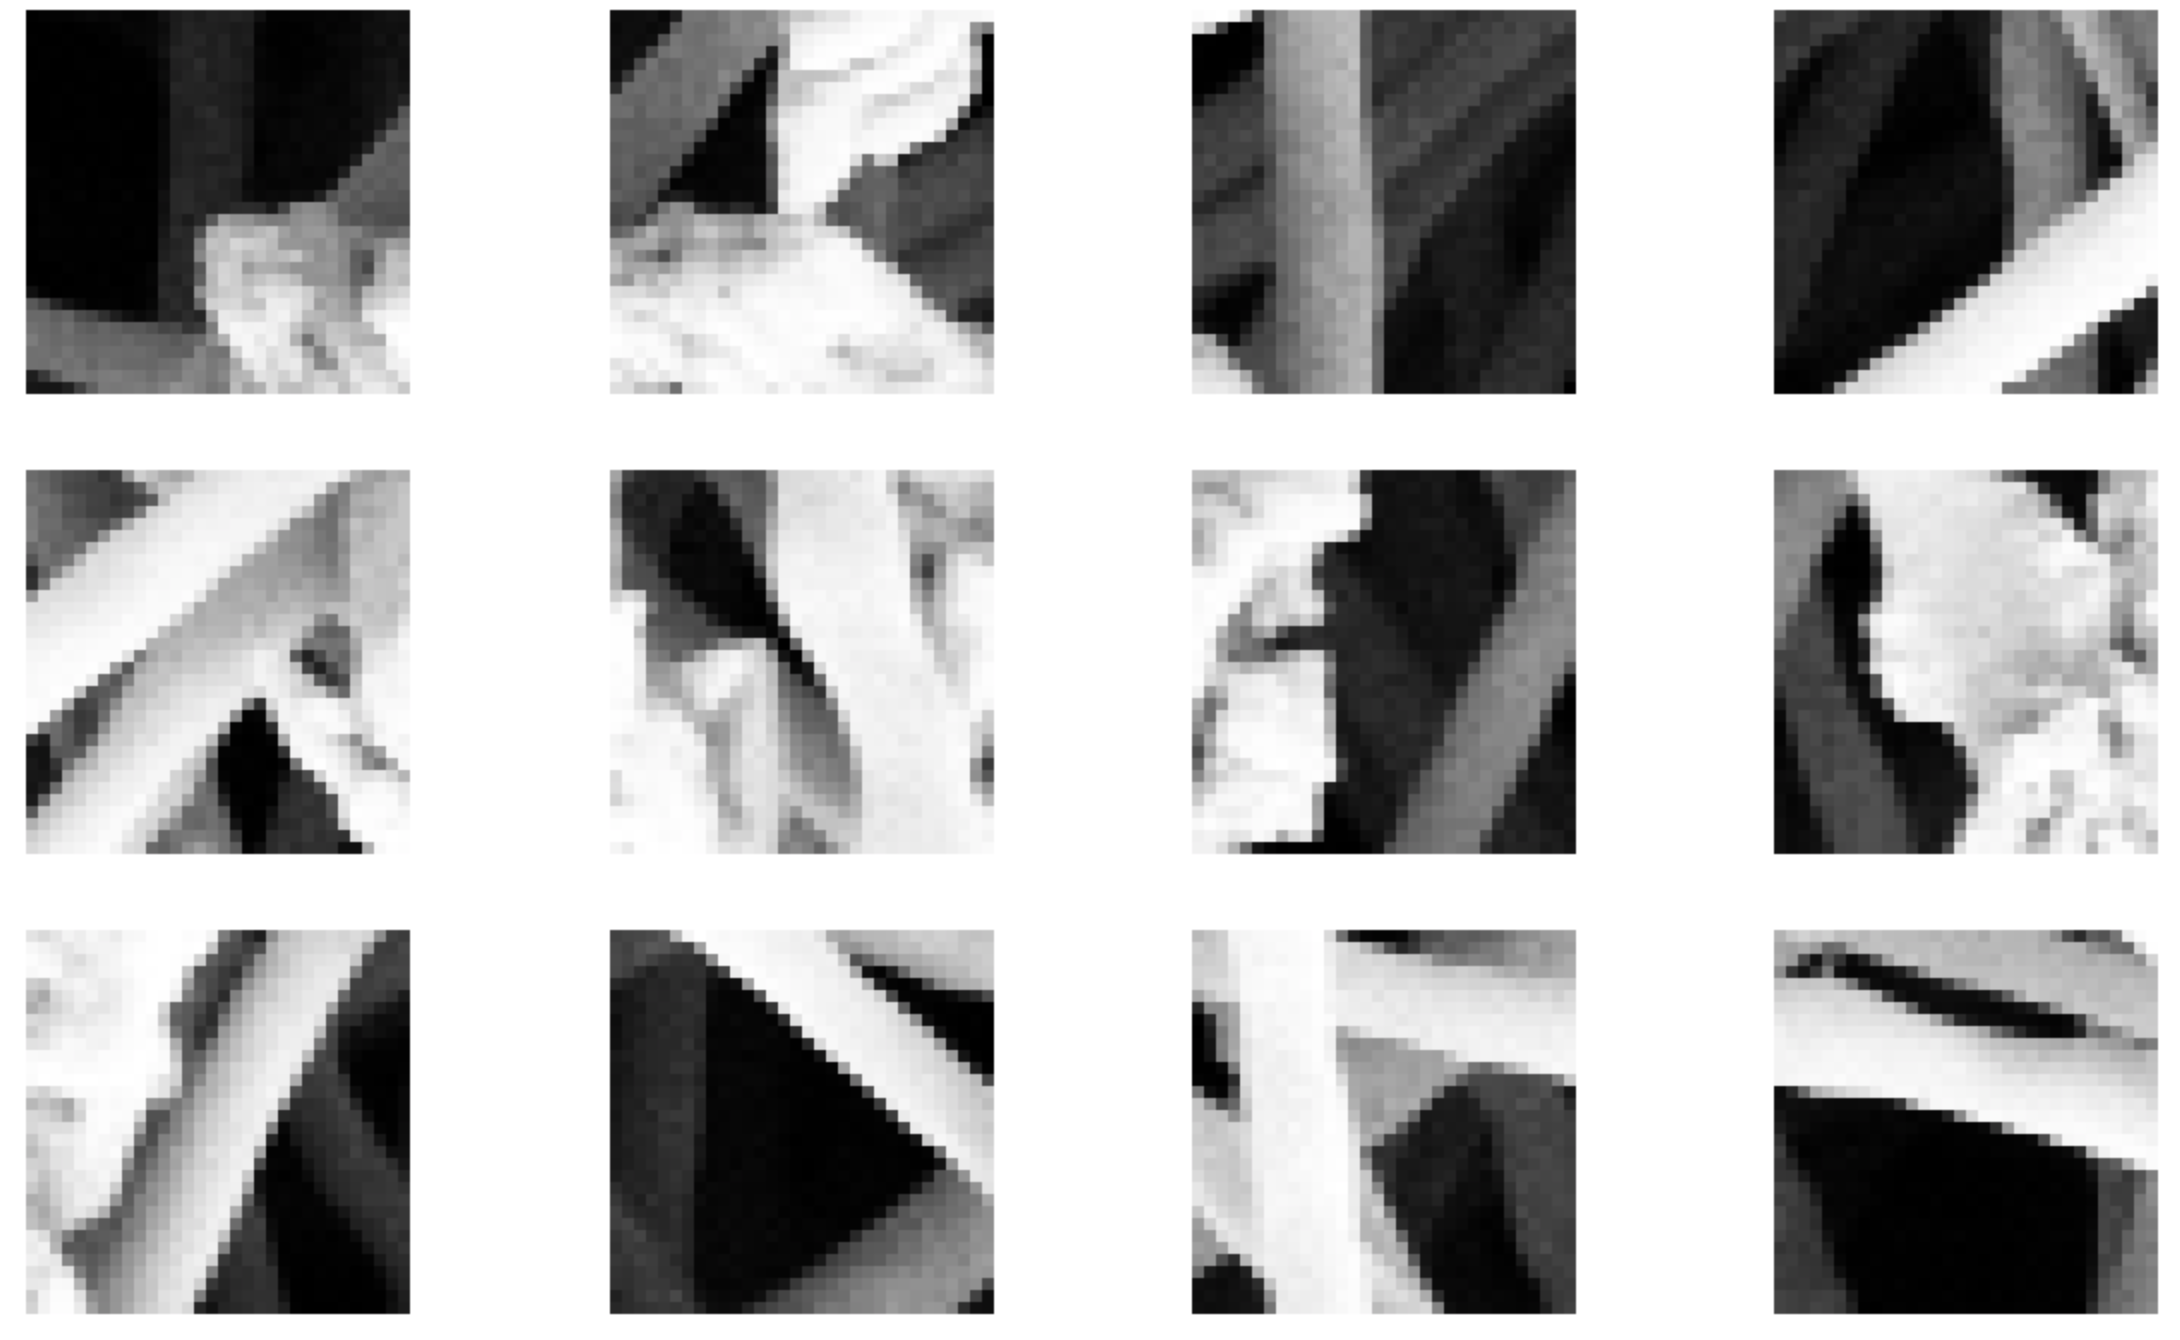
\includegraphics[width=1\textwidth]{sample_anomaly}}
			\label{fig:data_sample_anomaly}
	\end{minipage}}
	\caption{Normal and Anomalous region patches for the training and testing}
	\label{fig:data_samples}
\end{figure}

$32 \times 32$ patches are selected as the image size as if proposed framework prove useful for the
anomaly detection, testing the model with other known datasets such as CIFAR10 \cite{cifar10} and
SVHN \cite{Netzer2011ReadingDI} would be more convenient. $28 \times 28$ patch size is also
considered but choosing $28 \times 28$ image size forced model to have less transposed convolution
layers (see chapter \ref{chap:imp_details} for model details) and GAN models designed with that
architecture experienced model collapse frequently in the preliminary experiments. Figure
\ref{fig:data_sample_normal} shows the example patches used for the training phase. Training dataset
consists of patches which contains no anomalies. Figure \ref{fig:data_sample_anomaly} shows the
anomalous samples which are used in the inference stage. The Anomalous regions can reside in both
the topmost layer or can be hidden in deep in the woven structure.

\section{Analysis of Aforementioned Approaches}
\label{sec:analysis_before}

This section presents an analysis on the performance of GAN based state of the art anomaly detection
methods presented in section \ref{sec:gan_based_sota} and a discussion to identify the shortcomings
of these methods. Stabilization issues in the adversarial training stage, reconstruction problems
related to the encoding of latent representation and the method of computing the anomaly score will
be discussed. While discussing these issues, the proposed model will be introduced incrementally by
addressing the modifications and measures to mitigate the affect of these shortcomings to the
performance.

Proposed methods in chapter \ref{chap:sota} can be further divided into 2 seperate categories with
respect to their generator structure. 
\begin{itemize}
	\item Pure GAN ( AnoGAN (\ref{sec:anogan}), BiGAN (\ref{sec:bigan}) and ALAD (\ref{sec:alad}))
	\item Autoencoder Variants (GANomaly and Skip-GANomaly (\ref{sec:ganomaly}))
\end{itemize}

First group has a generator that accepts the noise as an input and uses adversarial training to
match the generated sample distribution to the input data distribution. The latter uses an
autoencoder based decoder in favor of the generator but still employs adversarial training to learn
the latent representation. During the analysis of the first two observations, autoencoder variants
will not be considered for discussion since their generator network does not suffer from the
stabilization issues of GANs.

\subsection{Stabilization of Adversarial Training}

Generator and discriminator's objective function stabilization is still an important issue in GAN
training. Various approaches and modifications are experimented to further improve the training of
the GANs and prevent non convergent scenerios. \cite{methods} and \cite{fm} proposed additional
stabilization "tricks" to improve the convergence properties of the objective function and prevent
mode collapse. These include adding noise with a decay over time to both input image and generated
sample before putting through discriminator to add a factor of robustness to the discriminator,
using soft labels to define the true and fake member class instead of the binary truth values and
flipping labels of the true and generated images to fool the discriminator even more and provide
higher gradient flow to generator early on in the training to help it learn to generate images
better \cite{fm}.

In the training phase of an generative adversarial network, loss values of generator does not
portray a traditional convergence line in plots. Adversarial minimax game prevents the losses of the
player networks to converge to a certain limit. If the loss is reaching zero in any case, it
indicates a problem in the learning capacity of one of the networks. If discriminator loss converges
to zero too quickly, it means that it learned to discriminate between the real images and the ones
generated by the generator network. On the other hand if the generator loss converges to zero early
in the training  it indicates a mode collapse but situation may arise in even normal looking
training sessions. The problem is at some point in the training generator generates an image that
perfectly fools the discriminator. If gradients obtained from this loss computation is high enough,
generator might stop learning from the gradient flow of discriminator and start to generate the same
sample in each iteration. This sample also may not be visually similar to the target distribution.
This eliminates the purpose of having a generator network.

To mitigate these shortcomings, ablation study is performed on all Pure GAN models which consists of
previously mentioned training improvements with same model capacity and training hyperparameters to
create an equal environment for the models. Despite models proving a certain performance standard on
the benchmark datasets (\cite{cifar10,Netzer2011ReadingDI}), they performed poorly on the SEM image
dataset (\cite{sem}). More importantly, the training of the networks were unstable enough to prevent
to obtain a consistent performance benchmark. Obtaining a stable GAN for generating reconstructions
is fairly important because it is the first step of the anomaly detection framework. Figure
\ref{fig:arim_training} presents the generator/discriminator learning graphs and their generation
samples from the final training epoch.

% Figure with bigan alad anogan graphs and reconstructions
\begin{figure}[h!]
\def\tabularxcolumn#1{m{#1}}
\begin{tabularx}{\linewidth}{@{}XXX@{}}
	\begin{tabular}{ccc}
		\subfloat[AnoGAN generator training]{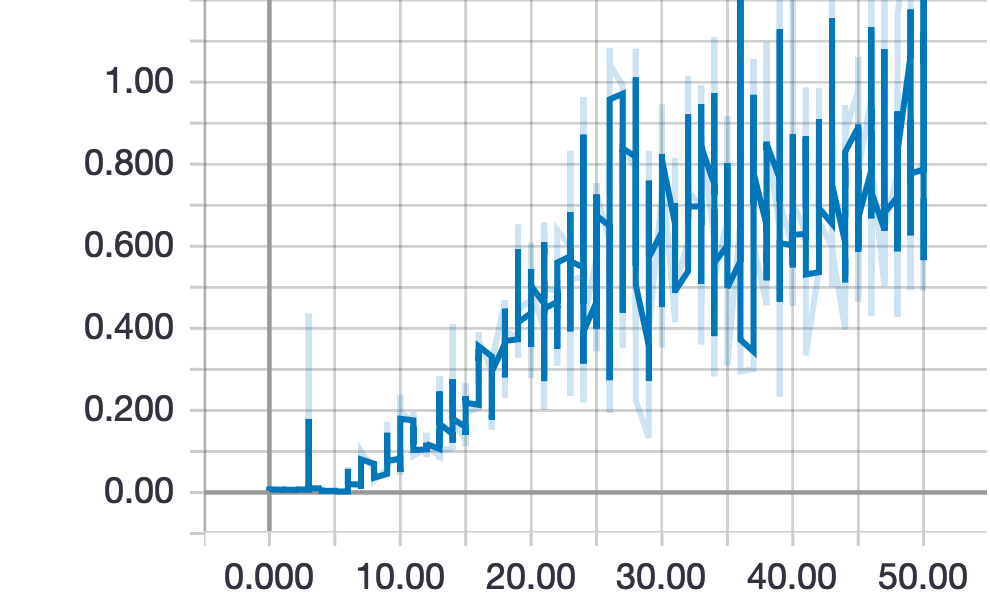
\includegraphics[width=0.3\textwidth]{arim/gan_training/anogan_loss_generator}} 
		& \subfloat[BiGAN generator
		training]{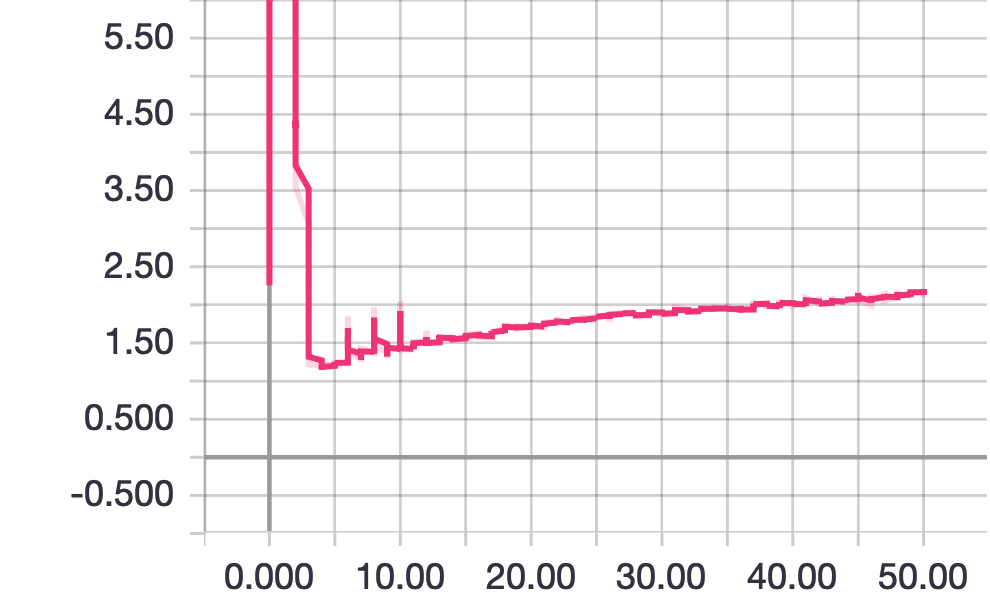
\includegraphics[width=0.3\textwidth]{arim/gan_training/bigan_loss_generator}} &
		\subfloat[ALAD generator
		training]{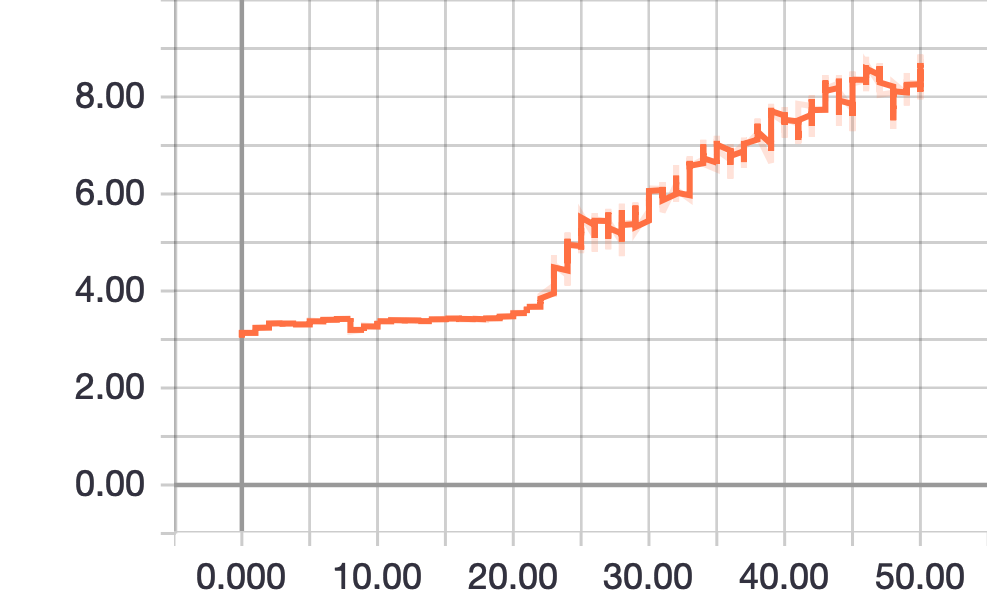
\includegraphics[width=0.3\textwidth]{arim/gan_training/alad_loss_generator}} \\
		\subfloat[AnoGAN discriminator training]{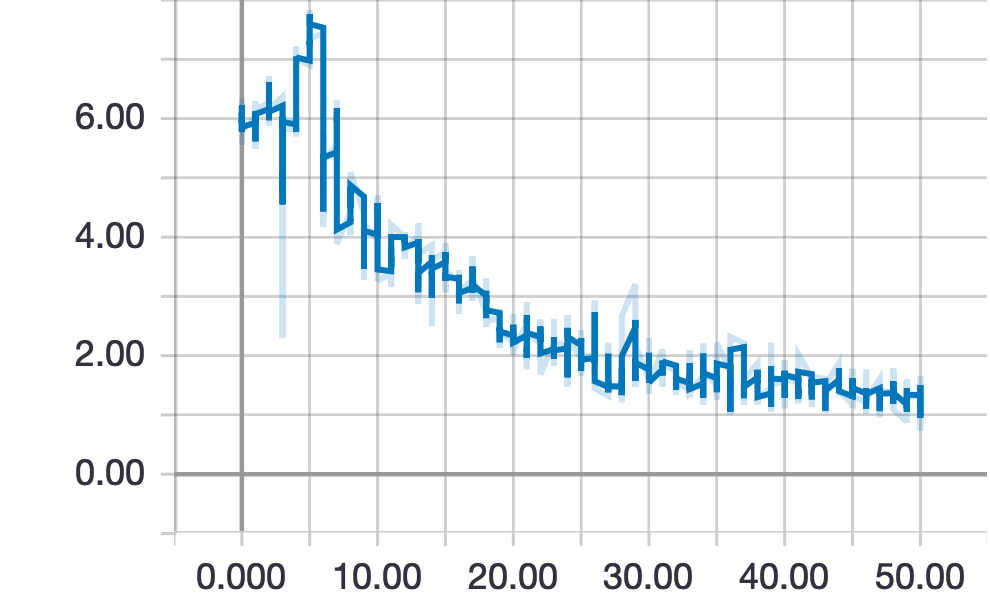
\includegraphics[width=0.3\textwidth]{arim/gan_training/anogan_loss_discriminator}} 
		& \subfloat[BiGAN discriminator
		training]{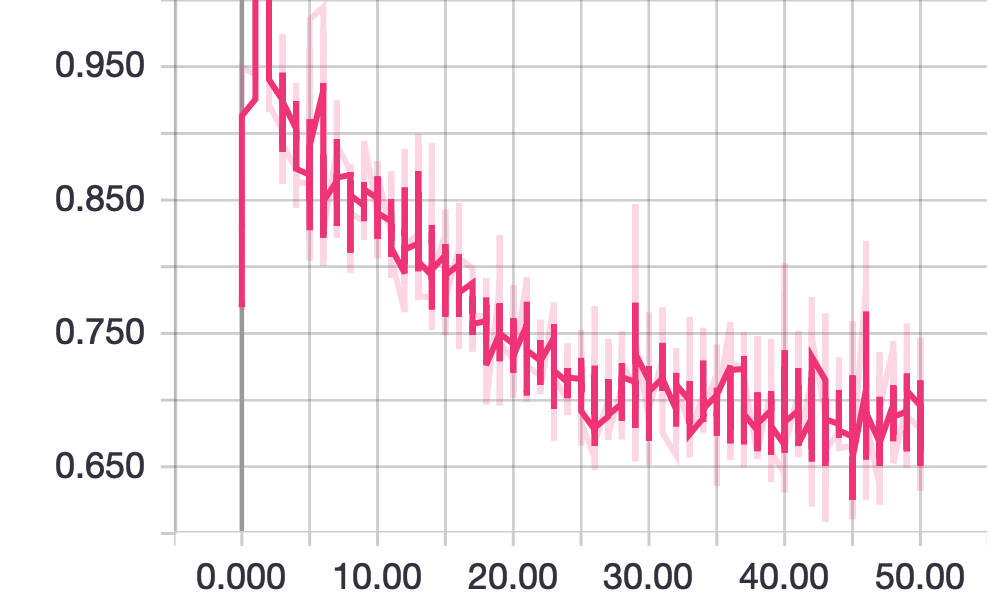
\includegraphics[width=0.3\textwidth]{arim/gan_training/bigan_loss_discriminator}}
		& \subfloat[ALAD discriminator
		training]{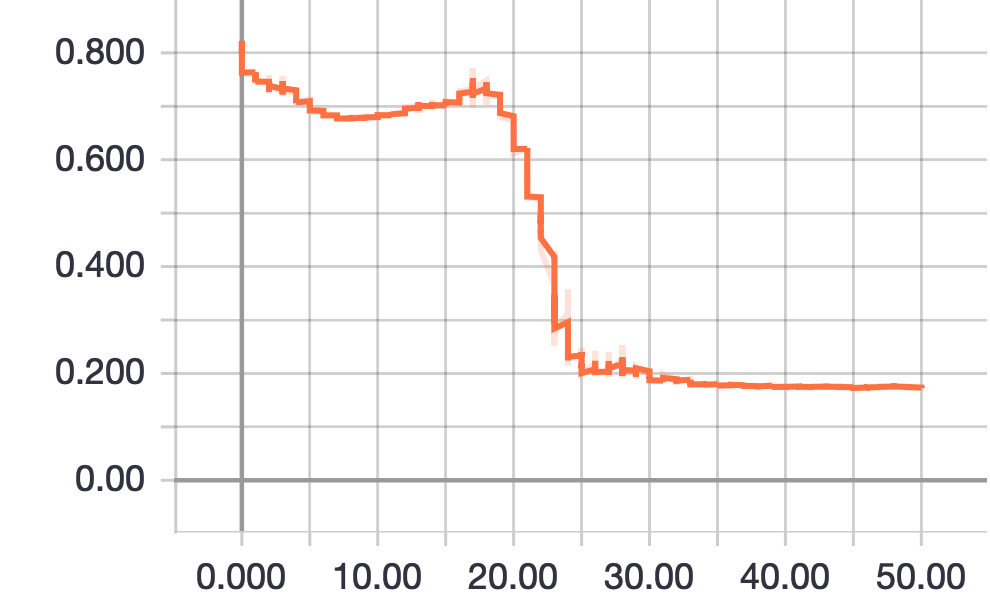
\includegraphics[width=0.3\textwidth]{arim/gan_training/alad_loss_discriminator}}
		\\
		\subfloat[AnoGAN generated image sample]{
\includegraphics[width=0.3\textwidth]{arim/gan_training/anogan_gan}} 
		& \subfloat[BiGAN generated image
		sample]{
\includegraphics[width=0.3\textwidth]{arim/gan_training/bigan_gan}} & \subfloat[ALAD
		generated image sample]{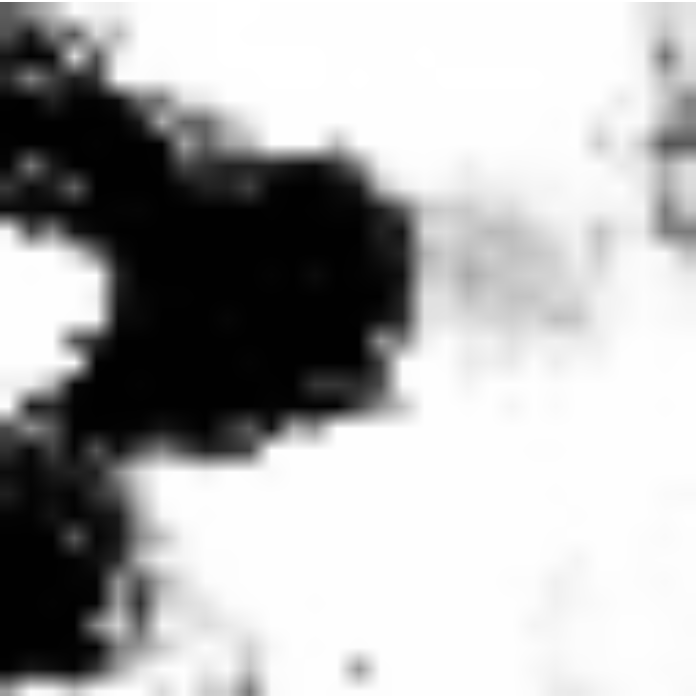
\includegraphics[width=0.3\textwidth]{arim/gan_training/alad_gan}}
	\end{tabular}
	\end{tabularx}
	\caption{Training information for the Pure GAN models. For graphs, x axis is the number of epochs and the y axis is the loss value}\label{fig:arim_training}
\end{figure}
%%%
As seen in the figure, discriminator is gradually learning to differentiate between the real and
generated image while the generator network does not seem to set its loss to a certain level as
desired. This trend is observed in the majority of the experiments and in the ablation study as
well. From the perspective of the image generation, samples generated from GANs are not contextually
sound enough to represent the target distribution of the SEM image dataset. To obtain a more concise
observation the reconstructions of these GANs will also be inspected. 
\begin{equation}
\label{eqn:ebgan_used}
\begin{aligned}
D(x)&=\|\operatorname{Dec}(E n c(x))-x\|\\[5pt]
V(G, D) &= D(G(z)) + D(x)+[m-D(G(z))]^{+} \\[5pt]
\mathcal{L}_{D}(x, z) &=D(x)+[m-D(G(z))]^{+} \\[5pt]
\mathcal{L}_{G}(z) &=D(G(z))
\end{aligned}
\end{equation}
Considering the results of these experiments, training objective of the EBGAN model is adopted to
obtain a more stable training with our dataset.  (See eqn. \ref{eqn:ebgan_used})


Defining loss function as a value of energy still preserves the adversarial aspect of the objective
function. An auto encoder network acts as a discriminator module and attains an energies to the real
and fake image samples with high energy values assigned to generated images. Generator tries to
"fool" the discriminator to decrease the amount of energy fake image is assigned. Here the energy
term is described as the ability of discriminator to reconsturct the given output, so it is a
reconstruction error based value. 

Using energy based GAN proved useful to obtain a consistent performance without having issues with
argued stabilization problems. Details regards to its training and model's reconstruction capability
will be discussed in its own section.
\subsection{Convergence of Encoder Training}
\label{sec:conv_enc}

Stabilizing the GAN training is actually the second step for a reconstruction based anomaly
detection approach. As proposed, generator network learns the mapping from the latent space $Z$ to
the image space $X$. However in order to test unknown images for anomalies, the latent
representation of the image must be extracted. From this point on this operation is called the
"inverse mapping". Generators are not able to provide this kind of inverse mapping so pure gan based
models followed different approaches to obtain this information.

AnoGAN model implements a backpropagation routine for a predetermined number of steps to approximate
the latent representation of the query image. It randomly initializes a latent representation vector
and updates it until the loss that is defined as the $\ell_{2}$ norm of the query image and
generated sample converges. The main disadvantage of this approach is the time constraint. Method
works with image patches so processing whole image takes a considerable amount of time compared to
other methods.

BiGAN and ALAD on the other hand, adds an additional encoder network to their adversarial training
to learn the inverse mapping while learning the image distribution (see eqn.
\ref{eqn:alad_bigan_eqn}).
\begin{equation}
\label{eqn:alad_bigan_eqn}
\begin{aligned} V\left(D, E, G\right) &=\mathbb{E}_{x \sim p_{\text{data}}}\left[\log D_{x z}(x, E(x))\right] \\ &+\mathbb{E}_{z \sim p_{Z}}\left[1-\log D_{x z}(G(z), z)\right]
\end{aligned}
\end{equation}

To learn both mappings, models learn the joint probability distribution of the image and the noise
pairs. Discriminator network therefore is modified to process this new representation (see
implementation details in appendix \ref{app:bigan} and \ref{app:alad}). Integrating an encoder
network solves the time constraint problem because the latent representation is acquired with
feeding the query image to the encoder network at the inference stage and the computation time is
negligible compared to AnoGAN's approximantion. Nonetheless addition of a new component to the
adversarial training brings new stabilization problems with regards to encoder network. Training of
the generator discriminator, implicitly affects the quality of the representation encoded. ALAD
implements additional discriminators to control the conditional probability distributions of the
learned joint distribution from both ends (For noise and for image) to improve the encoder
performance but experiments did not provide a considerable advance even with ablation study. Figure
\ref{fig:arim_encoder} presents the training graphs of the models and their obtained
reconstructions. AnoGAN model does not have a training graph for encoder since it uses a
backpropagation and it would have a convergence graph for each patch in the dataset. Instead, the
training graph of the first iteration of the proposed model's encoder is presented. 
\begin{figure}[h!]
	\def\tabularxcolumn#1{m{#1}}
	\begin{tabularx}{\linewidth}{@{}XXX@{}}
		\begin{tabular}{ccc}
			\subfloat[BiGAN Encoder Training]{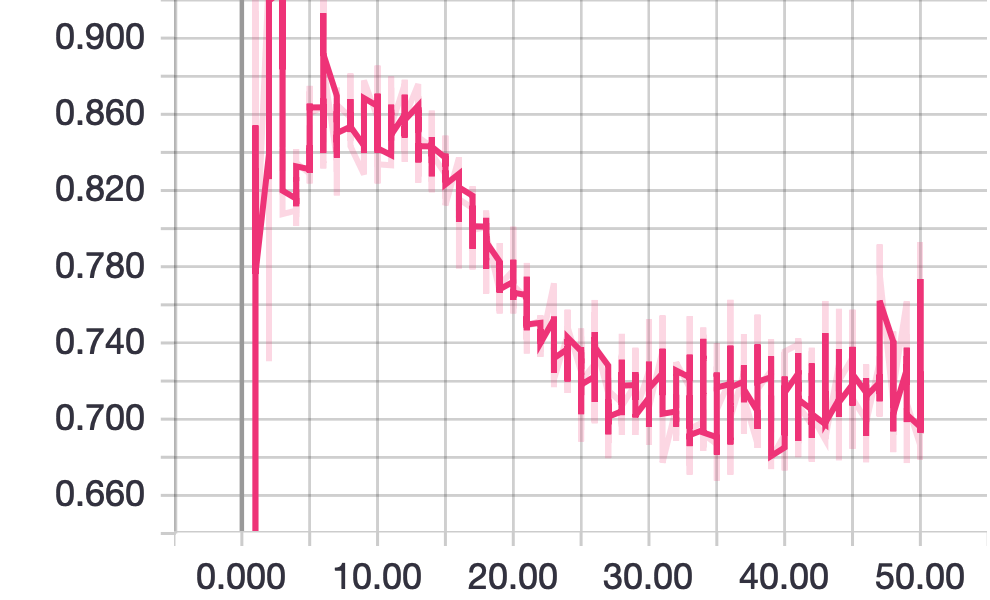
\includegraphics[width=0.3\textwidth]{arim/encoder_conv/bigan_loss_encoder}} 
			& \subfloat[ALAD Encoder
			Training]{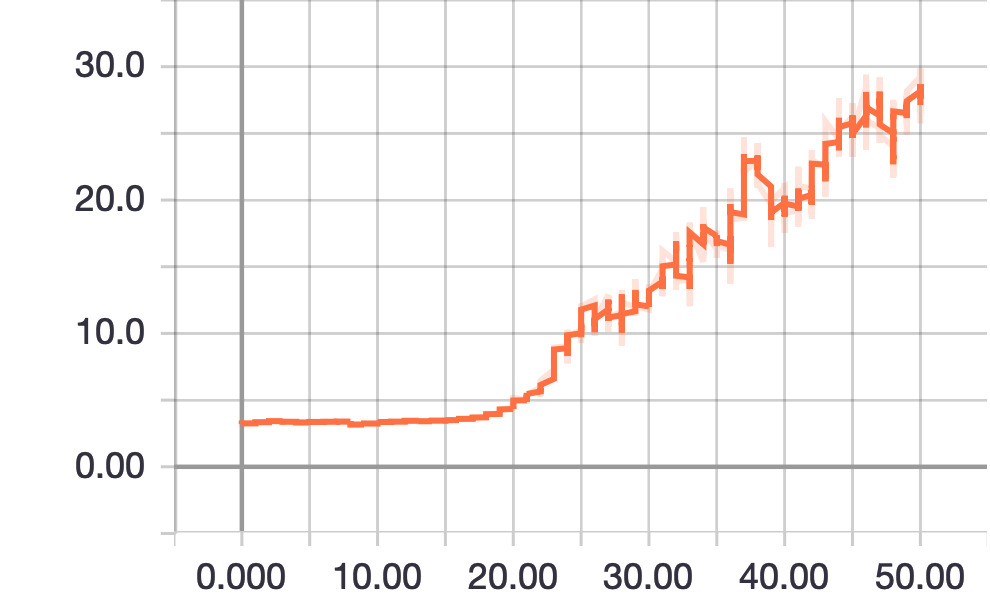
\includegraphics[width=0.3\textwidth]{arim/encoder_conv/alad_loss_encoder}} &
			\subfloat[ENCEBGAN Encoder
			Training]{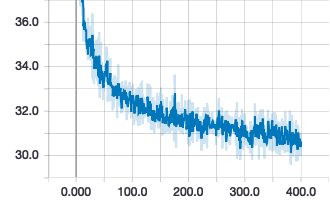
\includegraphics[width=0.3\textwidth]{arim/encoder_conv/enceb_loss_encoder}}
			
		\end{tabular}
	\end{tabularx}
	\caption{Training graphs of pure GAN models that implement encoder network and the first iteration of the proposed network}\label{fig:arim_encoder}
\end{figure}

By itself, these training graphs does not give us a reliable insight about encoder performance.
Other than its quantative results, encoder networks performance can be quantified with models'
ability to reconstruct a given image after training. At this point in pipeline, impact of a good
generator also comes into play. In both models, the training of the encoder network is computed by
feeding the latent representation obtained from the encoder and feeding it to the generator to
reconstruct the training data. So performance and proper training of the encoder network also
depends on the adversarial training of generator. In the minimax game played by BiGAN and ALAD, both
encoder and generator tries to fool the discriminator. Therefore stabilization problem of generator
inadvertantly affects the encoder convergence which also affects the quality of the reconstructions
obtained from the model. Some distortions and the information loss is expected in the generator
based reconstruction. In our dataset, these imperfections cause reconstructed samples to be
interpreted as anomalous sample though the input is a normal sample. Figure
\ref{fig:arim_reconstruct} shows the reconstructions from AnoGAN, BiGAN and ALAD's inference stage. 

\begin{figure}[!ht]	
	\def\tabularxcolumn#1{m{#1}}
	\begin{tabularx}{\linewidth}{@{}XXX@{}}
		\begin{tabular}{ccc}
			\subfloat[AnoGAN Query Image]{
\includegraphics[width=0.3\textwidth]{arim/encoder_conv/anogan_sample}} 
			& \subfloat[BiGAN Query
			Image]{
\includegraphics[width=0.3\textwidth]{arim/encoder_conv/bigan_sample}} &
			\subfloat[ALAD Query
			Image]{
\includegraphics[width=0.3\textwidth]{arim/encoder_conv/alad_sample}} \\
			\subfloat[AnoGAN Reconstruction]{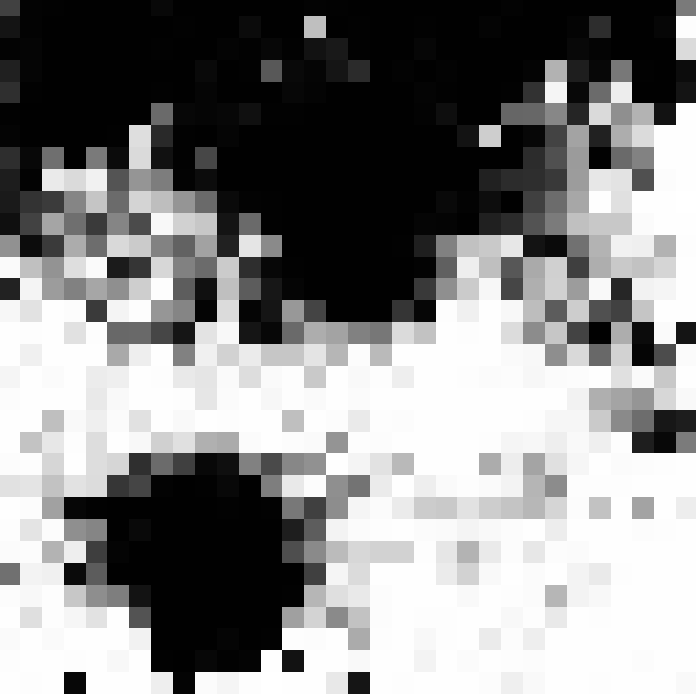
\includegraphics[width=0.3\textwidth]{arim/encoder_conv/anogan_reconstruct}} 
			& \subfloat[BiGAN
			Reconstruction]{
\includegraphics[width=0.3\textwidth]{arim/encoder_conv/bigan_reconstruct}}
			& \subfloat[ALAD
			Reconstruction]{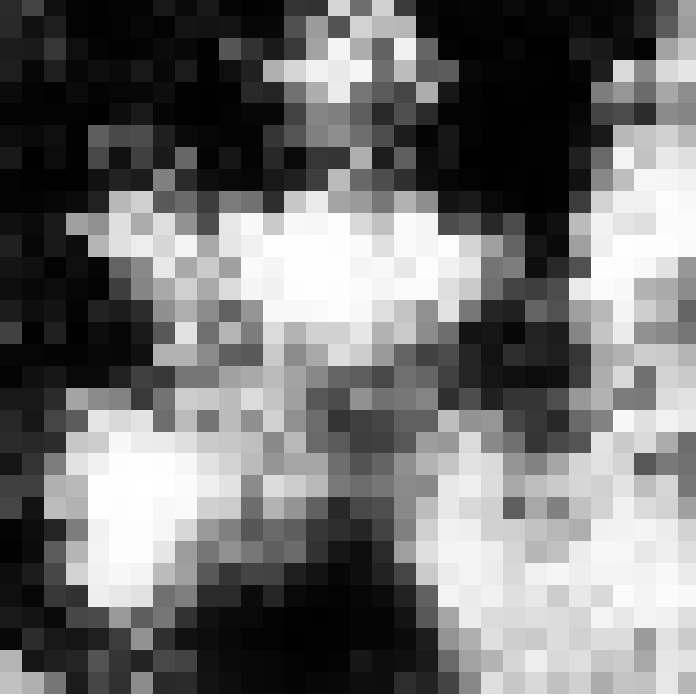
\includegraphics[width=0.3\textwidth]{arim/encoder_conv/alad_reconstruct}}
			
		\end{tabular}
	\end{tabularx}
	\caption{Reconstructed samples from the pure GAN models. Upper row is the given query image and the bottom row is their reconstructions}\label{fig:arim_reconstruct}
\end{figure}

Proposed model in this work also uses additional encoder network to get the inverse mapping
information. Several modifications are applied to the training in order to improve the stabilization
and ensure the convergence of the encoder. Eqn. \ref{eqn:ebgan_used} propose the modified generator
discriminator approach. Addition of the encoder network and its training is also based on an energy
based training.
\begin{equation}
\label{eqn:encebgan_used}
\begin{aligned}
D(x)&=\|\operatorname{Dec}(E n c(x))-x\|\\[5pt]
V(G,E, D) &= D(G(z)) + D(x)+[m-D(G(z))]^{+} + D(G(E(x))) \\[5pt]
\mathcal{L}_{E}(x) &= D(G(E(x)))
\end{aligned}
\end{equation}

Like AnoGAN and ALAD, proposed model also trains encoder network with generator networks help to
obtain the reconstruction. However, instead of training all the networks in the adversarial setting,
proposed model separates the trainig of the generator discriminator pair and the encoder network.
Training strategy presented in F-AnoGAN framework (see section \ref{sec:fanogan}) proposes an
initial adversarial training. In the second part of the training the encoder network is trained by
creating a pipeline with the other network components with fixed weights (inference mode) (See
figure \ref{fig:fanogan_training}). This approach focuses on the encoder training objective by
removing the dependency between encoder and generator which in turn also decreases the potential
stabilization issues of the generator network.

So far, configuring the models' objective function to an energy based setting and separating the
joint training into sequential steps give the model two opportunities:

\begin{itemize}
	\item The stabilization of the GAN training, which means better reconstruction performance.
	\item Easy convergence for encoder network because it isn't trained concurrently with the
	generator so learning latent reprensetation is uni directional gradient descent.
\end{itemize}

Next section will discussed the model with the mentioned changes and continue to analyze the
existent shortcomings despite the improvements.

\section{Encoded Energy Based Generative Adversarial Network}
\label{sec:encebgan}

The first iteration of the proposed model is called encoded energy based generative adversarial
network,or ENCEBGAN. This section presents how its built, its training scheme and the issues it
solved.

ENCEBGAN consists of an energy based generative adversarial network framework with an additional
encoder network. The roles of the networks are identical to BiGAN (\ref{sec:bigan}). Two main
differences are the change in the rationale in adversarial training component and separation of the
encoder network training. Figure \ref{fig:encebgan_model} presents the network components with an
emphasis on the training sequence.
\begin{figure}[h!]
	\centering
	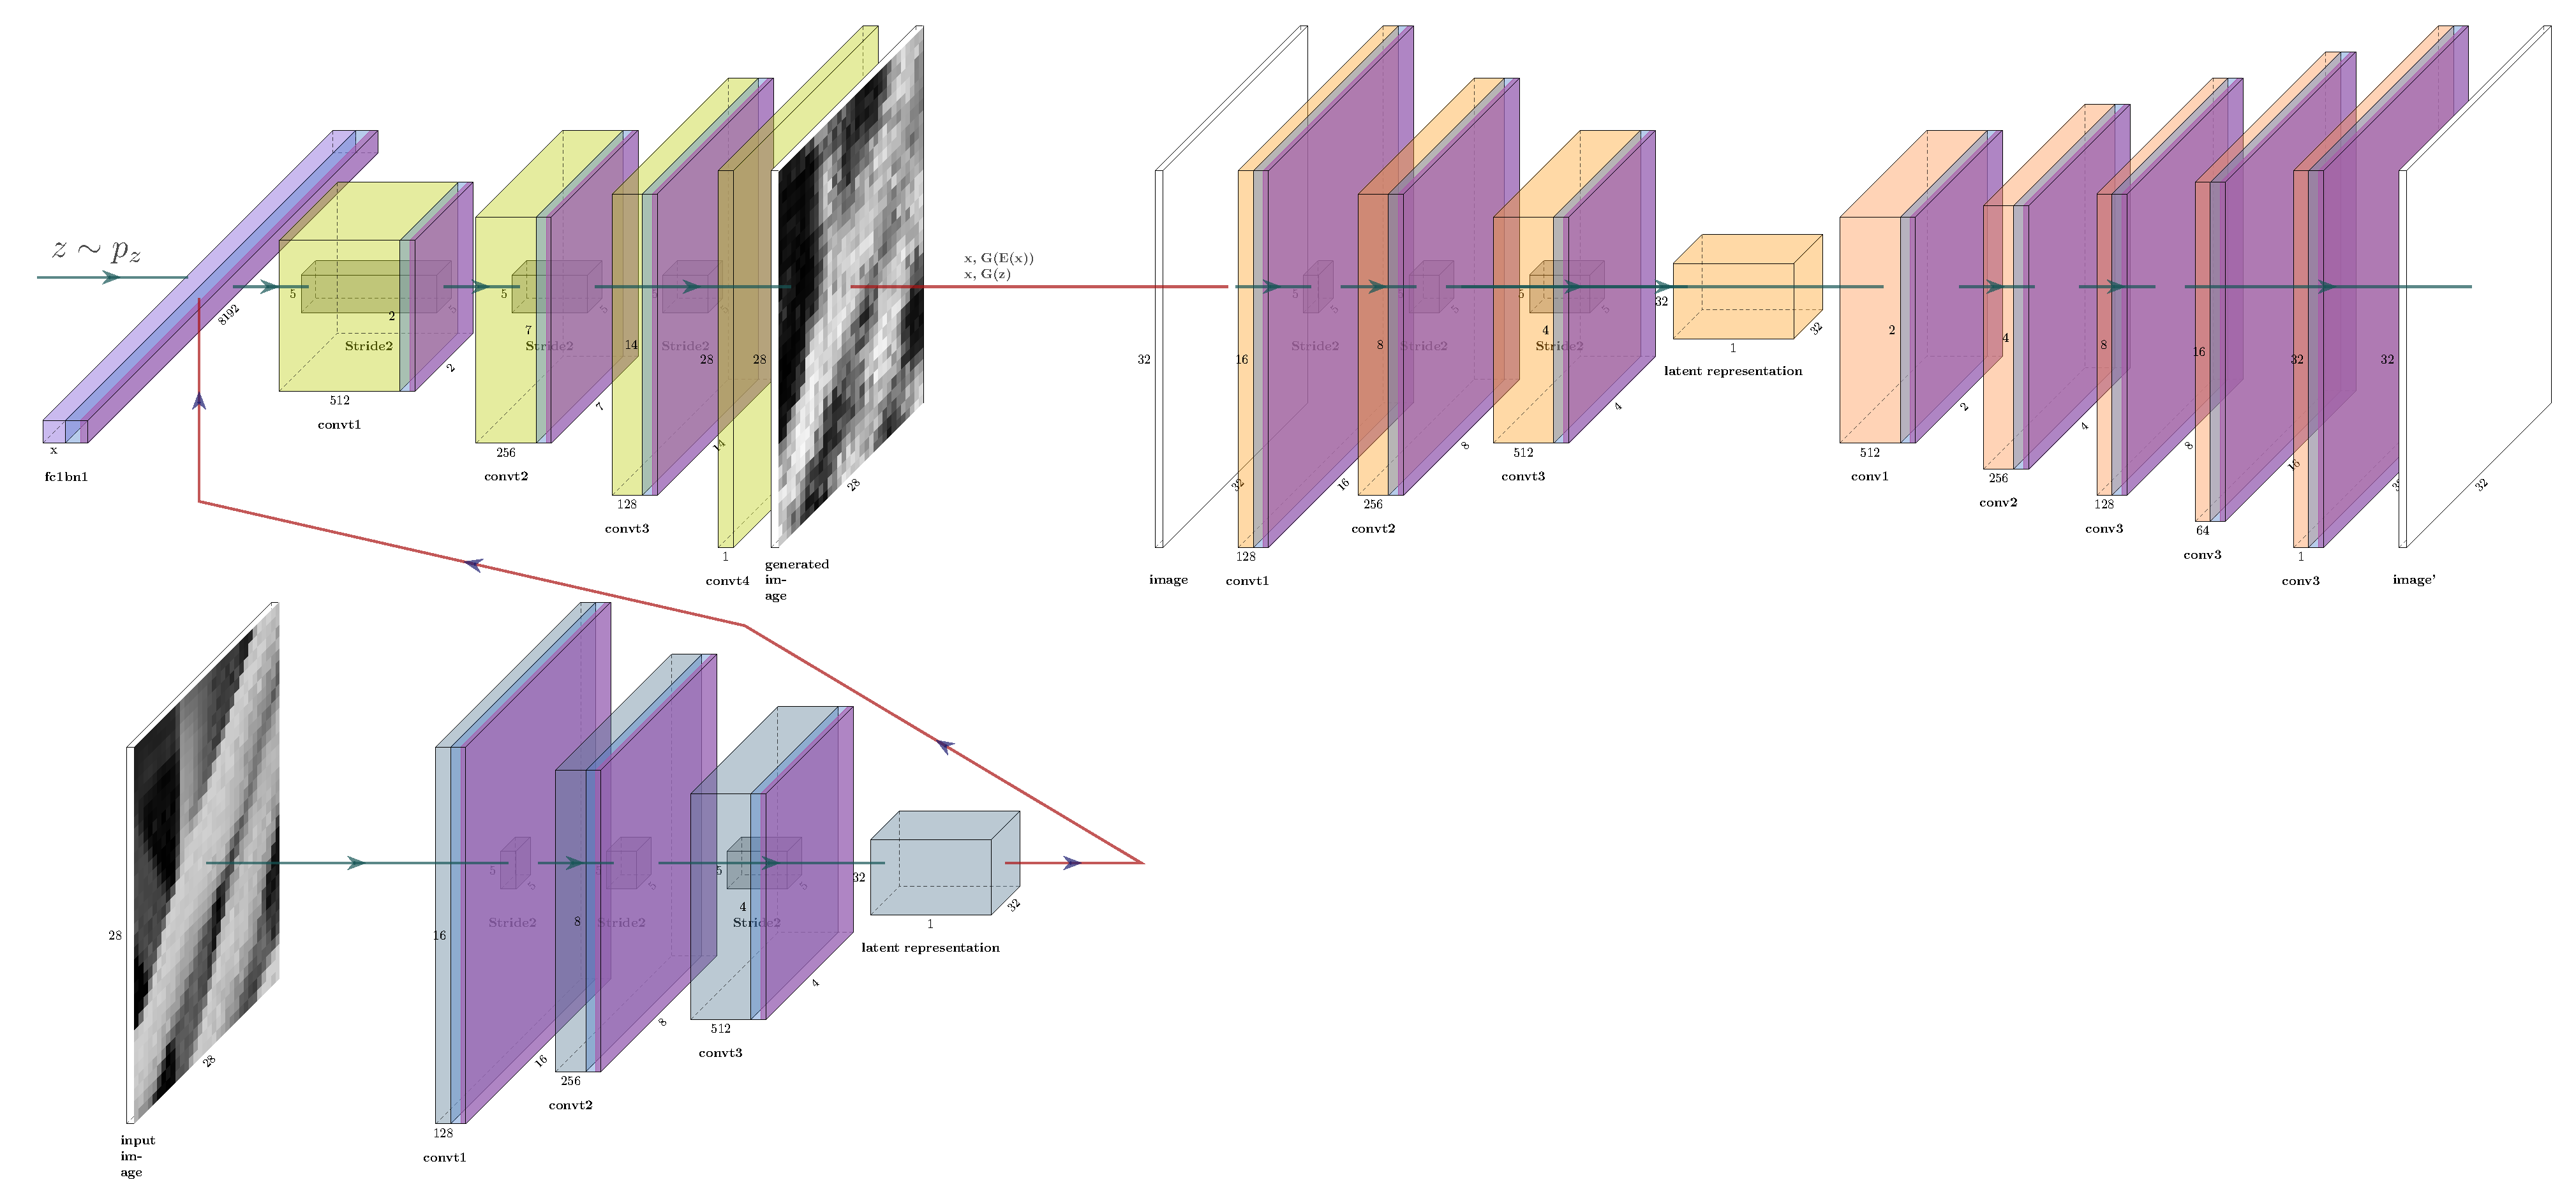
\includegraphics[width=1.0\textwidth]{arim/encebgan/encebgan}
	\caption{ENCEBGAN Model Overview }
	\label{fig:encebgan_model}
\end{figure}

Training of the model is divided into two sections. In the first section generator and discriminator
trains adversarially to learn the mapping from image space to latent space. While generator learns
the mapping, discriminator is concurrently learning to reconstruct the training dataset and learns
to encode the training data on its own. This latent representation will be used later on as an
auxilary information for anomaly score computation. After the adversarial training is completed,
pipeline is created from the encoder generator networks to form a conceptual autoencoder and whole
network is trained using the reconstruction error based objective function for the encoder network.
In second stage, generator and discriminator don't learn any additional information about the
dataset. This approach proved to be useful to stabilize both generator and encoder hence increased
the reconstruction quality of our model. Anomaly score computation is the same as the pure gan based
methods which is the reconstruction error between the query and the output of encoder generator
pipeline as depicted in equation \ref{eqn:enceb_ad}. 
\begin{equation}
	\label{eqn:enceb_ad}
	\mathcal{A}(x) = \norm{x - G(E(x))}^2
\end{equation}

Figure \ref{fig:arim_encebgan_info} presents the training graph information and reconstructed
samples as a comparison to reconstructions in figure \ref{fig:arim_reconstruct}.
\begin{figure}[!ht]	
	\def\tabularxcolumn#1{m{#1}}
	\begin{tabularx}{\linewidth}{@{}XXX@{}}
		\begin{tabular}{ccc}
			\subfloat[Generator Training Graph]{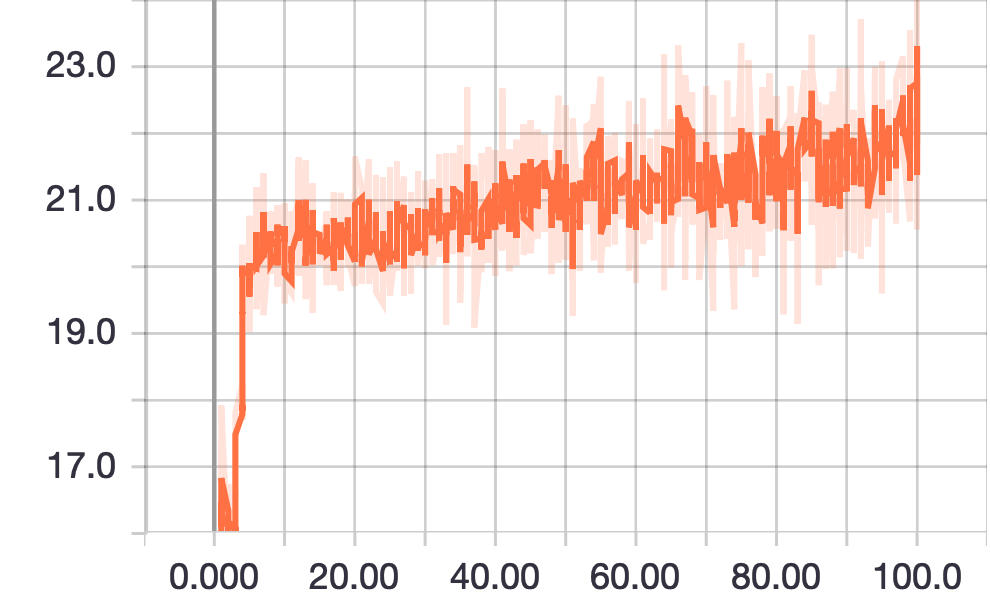
\includegraphics[width=0.3\textwidth]{arim/encebgan/encebgan_loss_generator}} 
			& \subfloat[Discriminator Training
			Graph]{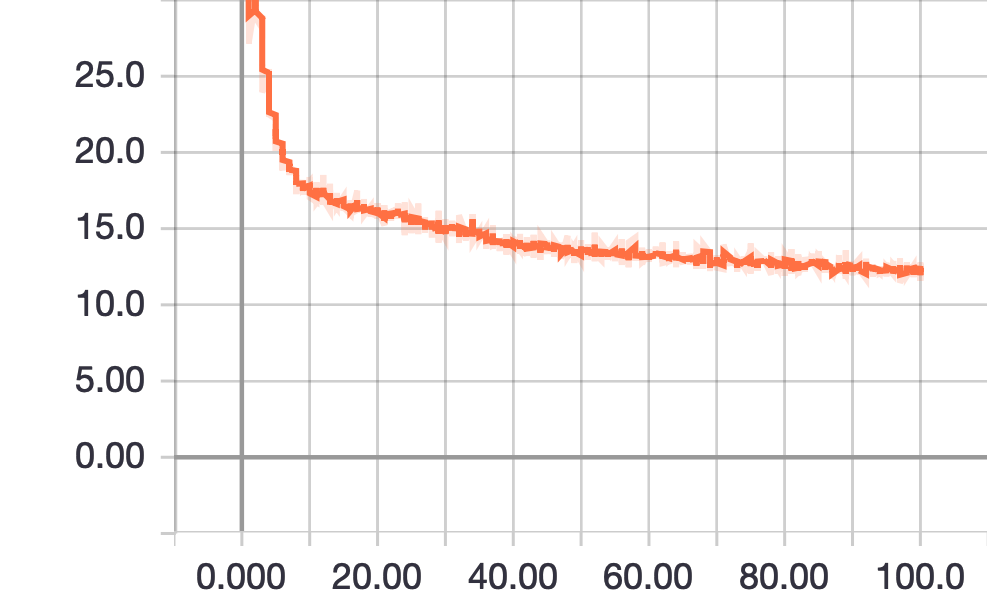
\includegraphics[width=0.3\textwidth]{arim/encebgan/encebgan_loss_discriminator}}
			& \subfloat[Encoder Training
			Graph]{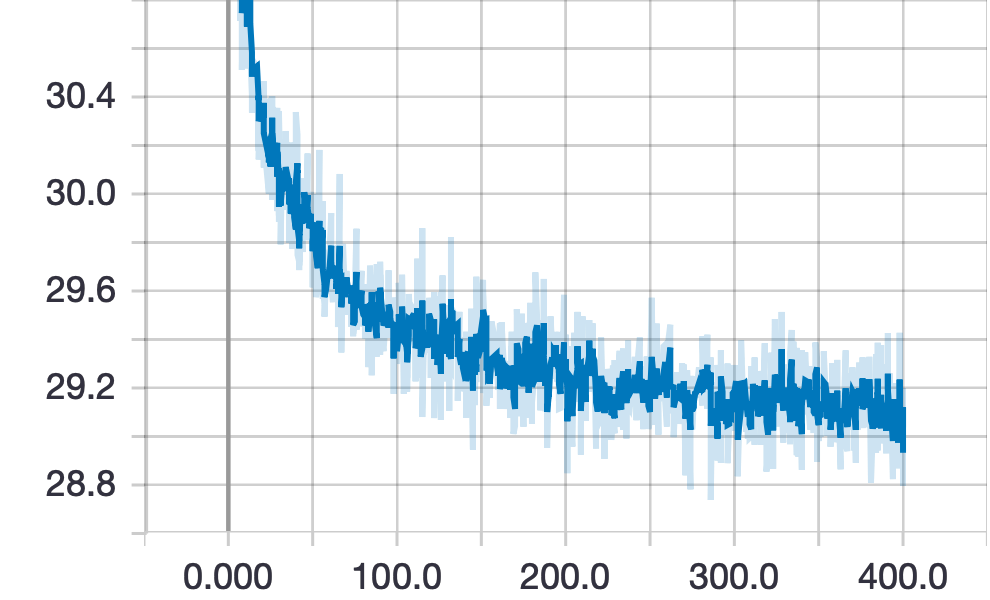
\includegraphics[width=0.3\textwidth]{arim/encebgan/encebgan_loss_encoder}} \\
			\subfloat[ENCEBGAN Generated Sample]{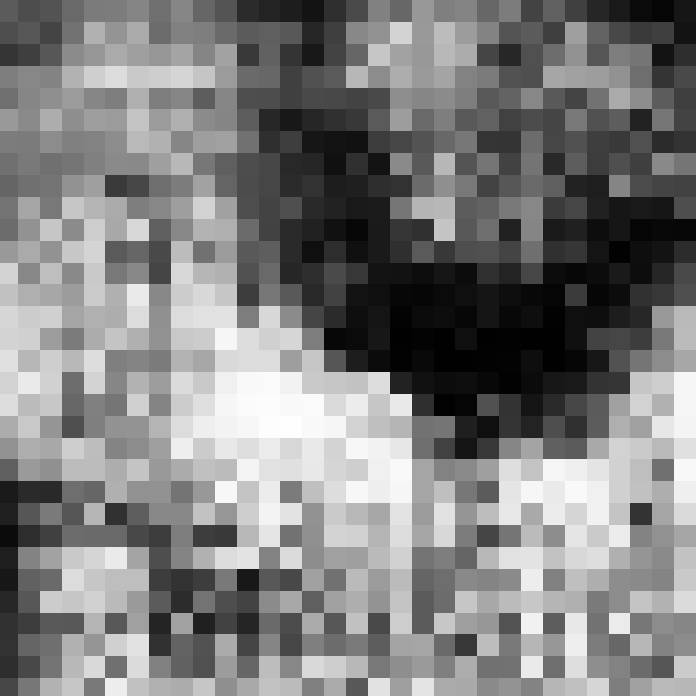
\includegraphics[width=0.3\textwidth]{arim/encebgan/encebgan_generated}} 
			& \subfloat[ENCEBGAN Query
			Sample]{
\includegraphics[width=0.3\textwidth]{arim/encebgan/encebgan_input}} &
			\subfloat[ENCEBGAN
			Reconstruction]{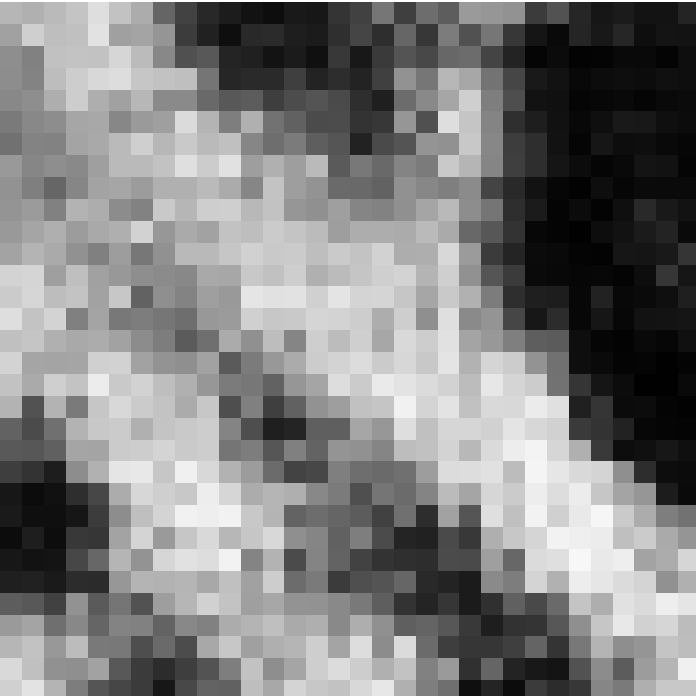
\includegraphics[width=0.3\textwidth]{arim/encebgan/encebgan_reconstruct}}\\
			
		\end{tabular}
	\end{tabularx}
	\caption{Training graphs and qualitative examples from ENCEBGAN Model}\label{fig:arim_encebgan_info}
\end{figure}

With previously mentioned architectural improvements, ENCEBGAN performed better than BiGAN and ALAD
and obtained the same performance as AnoGAN which will discussed in chapter \ref{chap:expres}.
Seperating the training of encoder and changing the adversarial objective function mechanics
consequently stabilized the convergence of both networks and the reconstruction quality has
increased compared to the pure gan based models.

Imperfections in the reconstructions are usually expected in reconstruction based anomaly detection
methods since the network trained to learn the latent representation is regularized to prevent
overfitting. In SEM image dataset, anomalous regions can occur in any level of the image with
varying levels of brightness. During the experiments of the models it is observed that,
imperfections in the reconstructions may be identified as anomalous regions even though the image is
anomaly free. This issue inadvertently cripples the anomaly detection performance of ENCEBGAN (and
other pure gan based models). 

Next section will discuss the anomaly score computation methods featured in both pure gan based and
autoencoder variant models, and explan the addition of a secondary encoder network to improve the
overall performance of the proposed model.

\subsection{Anomaly Score Computation}

% Why we divided Their difference
Previously we divided the state of the art gan based anomaly detection methods into two main
categories. Pure gan based models and autoencoder variants. The main difference between these groups
is that decoder (generator equivalent) network of these models is trained only with the latent
representation of the image supplied from the encoder network. Since they learn to reconstruct using
the encoded version of the training data, their reconstructions are superior compared to the pure
gan based methods. Figure \ref{fig:arim_anoscore} shows an example reconstruction from both GANomaly
and Skip-GANomaly \ref{sec:ganomaly}. 

\begin{figure}[!ht]	
	\def\tabularxcolumn#1{m{#1}}
	\begin{tabularx}{\linewidth}{@{}XXX@{}}
		\begin{tabular}{ccc}
			\subfloat[Query Sample]{
\includegraphics[width=0.3\textwidth]{arim/anomaly_score/anoscore_input}} 
			& \subfloat[GANomaly
			Reconstruction]{
\includegraphics[width=0.3\textwidth]{arim/anomaly_score/anoscore_ganomaly}}
			& \subfloat[Skip-GANomaly
			Reconstruction]{
\includegraphics[width=0.3\textwidth]{arim/anomaly_score/anoscore_sganomaly}}
			\\			
		\end{tabular}
	\end{tabularx}
	\caption{Reconstruction examples of Autoencoder Variant Models}\label{fig:arim_anoscore}
\end{figure}

Architectural difference between GANomaly and Skip-GANomaly is the additional skip connections
between the encoder and decoder network of the latter. This information transfer enables
Skip-GANomaly to retain more information about the data and help it to accumulate this data across
the layers during the decoding stage of the reconstruction. One interesting observation is that even
though the general quality of the Skip-GANomaly model is better than GANomaly on the SEM image
dataset, ablation study performed in chapter \ref{chap:expres}(see Table \ref{tab:ganomaly_ablation}
and \ref{tab:sganomaly_ablation}) shows that overall GANomalyprediction performance is superior
compared to Skip-GANomaly. 

Both anomaly score computation is based on the reconstruction based error, but GANomaly uses a
secondary encoder network to learn the latent representation of the reconstruction and uses this
information to compute the anomaly score (see eqn. \ref{eqn:ganomaly_as}). Skip-GANomaly on the
other hand composes the contextual data (reconstruction loss) with the latent loss which is obtained
from the feature layer of its discriminator network (see eqn. \ref{eqn:sganomaly_as}). We speculate
that training a secondary encoder network improved GANomaly model's interpretation of the anomalous
sample data. Erroneous predictions that are caused due to misinterpreting imperfect reconstructions
as samples that contains anomalous regions may be averted by interpreting both input image and its
reconstruction at the latent dimensional complexity. 

Considering these observations and related improvements, next section will present the final version
of the proposed model for anomaly detection. General architecture of the model, its training
procedure and its inference stage for anomaly detection will be discussed.

\section{Sequentially Encoded Energy Based Generative Adversarial Network}
\label{sec:sencebgan}

Sequentially encoded energy based generative adversarial network is the main proposed model that
aims to mitigate the disadvantageous outcomes of stabilization and convergence problems experienced
vy the previously mentioned methods (see chapter \ref{chap:sota}). Even though it is presented
incrementally throughout the chapter, its general architecture, training strategy and its approach
to anomaly detection problem will be discussed.
\begin{figure}[h!]
	\centering
	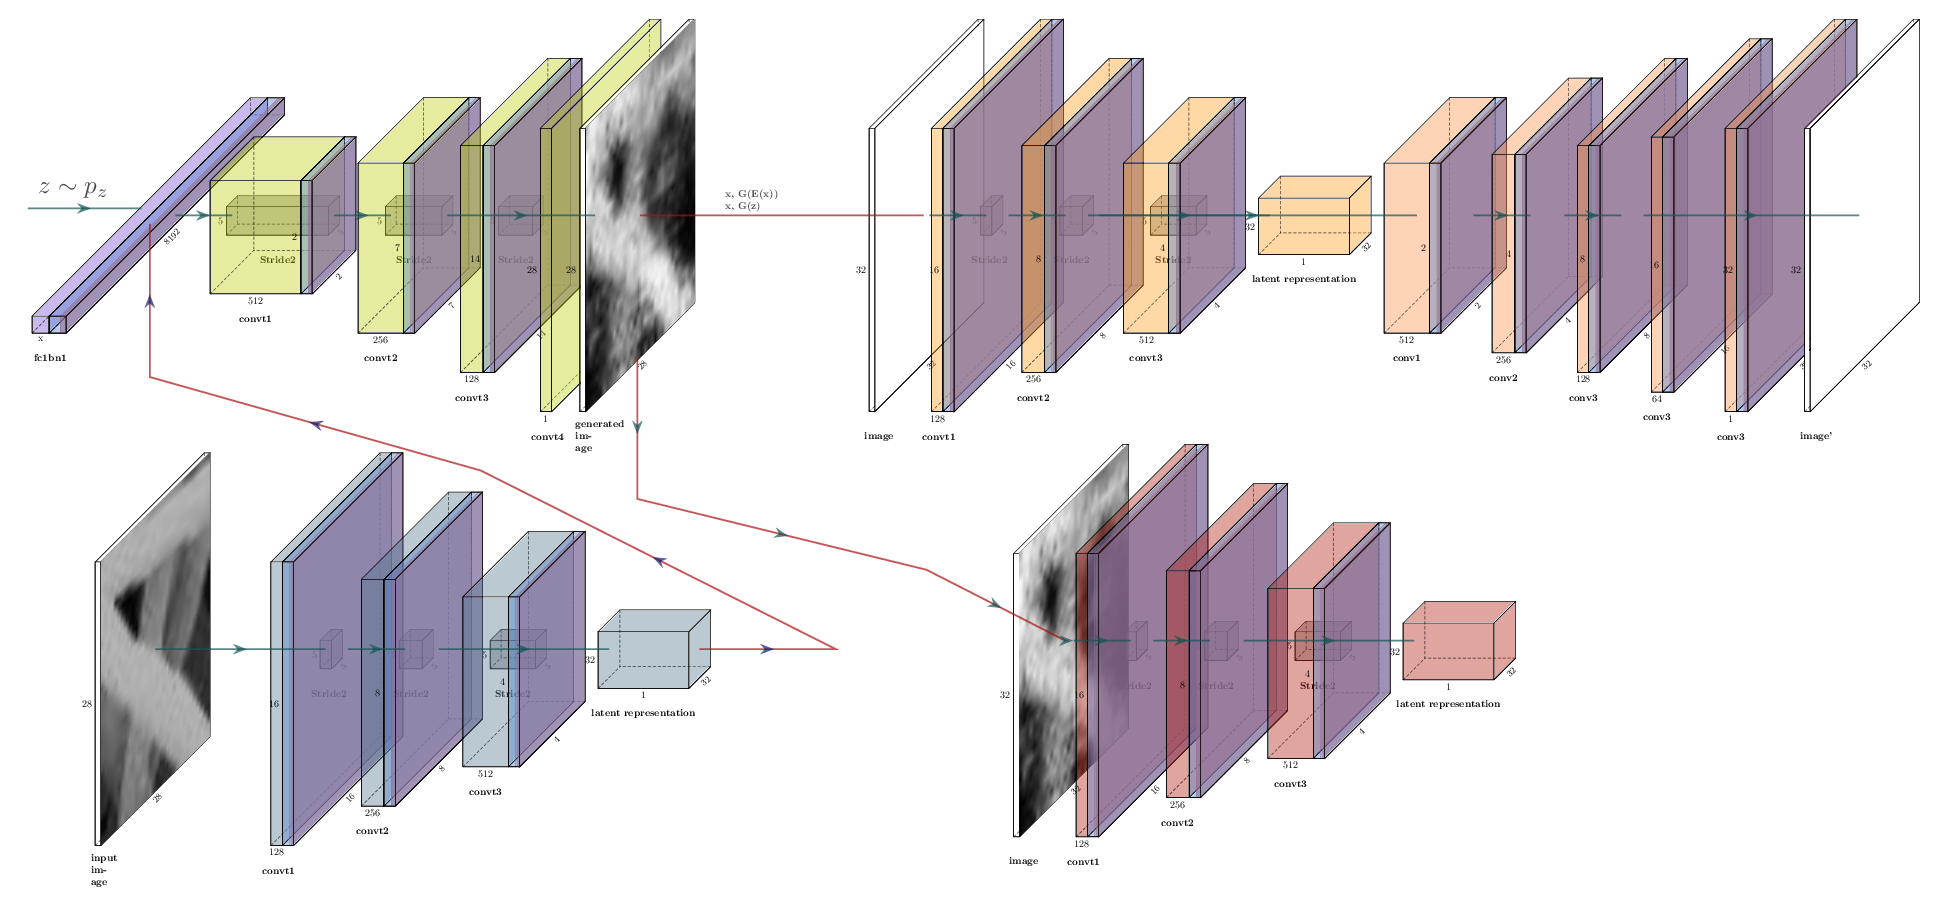
\includegraphics[width=1.0\textwidth]{arim/sencebgan/sencebgan}
	\caption{SENCEBGAN Model Overview }
	\label{fig:sencebgan_model}
\end{figure}

SENCEBGAN model consists of an energy based generative adversarial network and 2 additional encoder
networks. The first encoder network learns the representation of training data and its called
generator encoder or $E_{G}$. Second encoder learns the latent representation of the reconstructions
of the training data provided by the generator network. This encoder network will be mentioned as
reconstruction encoder or $E_{R}$. Training objective of the model is given in equation
\ref{eqn:sencebgan_formula}.
\begin{equation}
	\begin{aligned}
		D(x)&=\|\operatorname{Dec}(E n c(x))-x\|\\[5pt]
		V(G,E_{G},E_{R}, D) &= \underbrace{D(G(z))}_{\text{Generator}} + \underbrace{D(x)+[m-D(G(z))]^{+}}_{\text{Discriminator}} +\\ & \underbrace{D(G(E_{G}(x)))}_{\text{Encoder}_{G}} + \underbrace{\norm{E_{G}(x) - E_{R}(G(E_{G}(x)))}^2}_{\text{Encoder}_{R}}
	\end{aligned}
	\label{eqn:sencebgan_formula}
\end{equation}

Training objective is divided into three separate sequences. In the first stage of the training,
energy based gan framework is trained. After the training is completed, autoencoder architecture is
formed by merging $E_{G}$ and Generator $G$ with fixed weights. Combined with discriminator (also
fixed weights) $E_{G}$ is trained using the reconstruction error produced from the temporary
autoencoder configuration. In the last stage, $E_{R}$ is trained to learn the latent representation
of the reconstructed samples. Training is performed using the $\ell_{2}$ norm of the encoded
representation residual (see eqn. \ref{eqn:sencebgan_loss}). 
\begin{equation}
	\label{eqn:sencebgan_loss}
	\begin{aligned}
		\mathcal{L}_{E_{G}}(x) &= D(G(E(x))) \\[5pt]
		\mathcal{L}_{E_{R}}(x) &= \norm{E_{G}(x) - E_{R}(G(E_{G}))(x)}^2
 	\end{aligned}
\end{equation}

SENCEBGAN model separates anomaly detection computation into image based and latent dimension based
categories. Different anomaly score computations are tested to measure the impact of the additional
encoder networks and observe both implicit encoding and reconstruction capability of the
discriminator network. 
\begin{equation}
	\label{eqn:sencebgan_eqn_im}
	\begin{aligned}
	\mathcal{A}_{R}(x) & = \norm{x - G(E_{G}(x))}^ 2 \\[5pt]
	\mathcal{A}_{R_{D}}(x) & = \norm{D(x) - D(G(E_{G}(x)))}^2\\[5pt]
	\mathcal{A}_{IC}(x) & = \lambda \cdot \mathcal{A}_{R}(x) + (1 - \lambda) \cdot \mathcal{A}_{R_{D}}
	\end{aligned}
\end{equation}

Score functions defined in equation \ref{eqn:sencebgan_eqn_im} defines the anomaly measure using
spatial data. $\mathcal{A}_{R}(x)$ calculates the reconstruction error during the inference stage.
This anomaly score is the one used in all pure GAN based models. In order to test the reconstruction
capability of the discriminator $\mathcal{A}_{R_{D}}(x)$ score is employed. This score is calculated
by performing 2 consecutive reconstructions on the sample image. $\mathcal{A}_{IC}(x)$ is image
based combination anomaly score implemented to measure each of the image based anomaly scores'
affect on an ensemble approach.
\begin{equation}
	\label{eqn:sencebgan_eqn_z}
	\begin{aligned}
	\mathcal{A}_{L}(x) & = \norm{E_{G}(x) - E_{R}(G(E_{G}(x)))}^2  \\[5pt]
	\mathcal{A}_{L_{D}}(x) & = \norm{E_{G}(x) - L_{D_{Z}}(G(E_{G}(x)))}^2 \\[5pt]
	\mathcal{A}_{L_{D_{Z}}}(x) & = \norm{L_{D_{Z}}(x) - L_{D_{Z}}(G(E_{G}(x)))}^2 \\[5pt]
	\mathcal{A}_{LC}(x) & = \lambda \cdot \mathcal{A}_{L} + (1 - \lambda) \cdot \mathcal{A}_{L_{D_{Z}}} 
	\end{aligned}
\end{equation}

Secondary encoder network $E_{R}$ added to the model's pipeline enabled model to capability to
inspect the normality of query images in latent dimensional space and provided an alternative medium
regards to anomaly score computation. Inspired by the GANomaly model's (see sec. \ref{sec:ganomaly})
evaluation method, various types of anomaly score evaluations based on the latent representation
space is depicted in equation \ref{eqn:sencebgan_eqn_z}. $\mathcal{A}_{L}(x)$ measures anomaly score
based on the $\ell_{2}$ norm of the difference between encodings obtained during the pipeline.
Encoding capability of the discriminator network is also explored in these category.
$\mathcal{A}_{L_{D}}(x)$ and $\mathcal{A}_{L_{D_{Z}}}(x)$ scores tests the anomaly score by
comparing the latent representation obtained by the discriminator network. Finally, combined anomaly
score for latent represenation is employed to measure the affect of each score to an ensemble
methods. 
 
In terms of the performance, proposed model performed better than all previously mentioned models
except GANomaly. Performance analysis and observations regarding to its potential improvements and
different configurations will be explored in chapter \ref{chap:expres}.


\endgroup

%-------------------------------------------------------------------------------
\chapter{Experimental Results }
\label{chap:expres}
%!TEX root = ../2019_7_Ozgumus_Semsi_Yigit.tex

\begingroup

This chapter presents the performance of the gan based anomaly detection models and proposed model. 


\section{Experiment Settings}




\subsection{Performance Metrics}
This section will introduce the performance metrics used for the interpretation of the experiments performed.
These are:
\begin{itemize}
	\item Precision
	\item Recall
	\item F1 Score
	\item AUROC (Area Under Receiver Operating Characteristic curve)
\end{itemize}

 \textbf{Recall} is the ability of a model to find all the relevant cases within a dataset. In our case detection 
of all anomalies in a test would give us a recall of 1.0. \textbf{Precision} on the other hand is the ability 
ofa classification model to identify \textbf{only} the relevant data points. While recall expresses 
the ability to find all relevant instances in a dataset, precision expresses the proportion of the 
data points our model says was relevant actually were relevant. The calculation of the both metrics 
is given below
\begin{align}
\textbf{recall} & = \frac{\text{true positives}}{\text{true positives} + \text{false negatives}} \\[5pt]
\textbf{precision} & = \frac{\text{true positives}}{\text{true positives} + \text{false positives}}
\end{align}

Precision and recall comprises a trade off situation. If the model favors the precision, the recall 
decreases because eliminating the false positives inadvertently increases the false negative rate and 
vice versa. To give equal importance to both metrics, \textbf{F1 score} is used. The F1 score is the 
harmonic mean of precision and recall taking both metrics into account in the following equation:
\begin{equation}
\text{F}_{1} = 2 \times \frac{\text{precision} \times \text{recall}}{\text{precision} + \text{recall}}
\end{equation}

The last metric we use to interpret the model performance is area under receiver operating characteristic 
curve, \textbf{AUROC} for short. ROC curve visualizes the trade of relationship between the false positive 
and true positive rate. True positive rate is actually recall. False positive rate is the probability 
of false detection for the system. The calculations for these rates are provided below:
\begin{align}
\textbf{True Positive Rate} & = \frac{\text{true positives}}{\text{true positives} + \text{false negatives}} \\[5pt]
\textbf{False Positive Rate} & = \frac{\text{false positives}}{\text{true negatives} + \text{false positives}}
\end{align}

the AUROC value can be obtained by calculating the area under the ROC curve which has a range between 0 and 1 with a higher number indicating better classification performance.

\section{GAN Based Model Analysis}
% Anogan

\begin{table}[]
	\centering
	\caption{Ablation study for AnoGAN to test the effect of various training improvements for stabilization.}
	\label{tab:anogan_ablation}
	\resizebox{\textwidth}{!}{%
		\begin{tabular}{|c|l|llll|}
			\hline
			\multicolumn{2}{|c|}{\multirow{2}{*}{\textbf{Model}}} & \multicolumn{4}{c|}{\textbf{Metrics}} \\ \cline{3-6} 
			\multicolumn{2}{|c|}{} & AUROC & \multicolumn{1}{c}{Precision} & \multicolumn{1}{c}{Recall} & \multicolumn{1}{c|}{F1 Score} \\ \hline
			\multirow{8}{*}{AnoGAN} & Normal & \multicolumn{1}{c}{} & \multicolumn{1}{c}{} & \multicolumn{1}{c}{} & \multicolumn{1}{c|}{} \\ \cline{2-6} 
			& IN & \multicolumn{1}{c}{} & \multicolumn{1}{c}{} & \multicolumn{1}{c}{} & \multicolumn{1}{c|}{} \\ \cline{2-6} 
			& SL & \multicolumn{1}{c}{} & \multicolumn{1}{c}{} & \multicolumn{1}{c}{} & \multicolumn{1}{c|}{} \\ \cline{2-6} 
			& LF & \multicolumn{1}{c}{} & \multicolumn{1}{c}{} & \multicolumn{1}{c}{} & \multicolumn{1}{c|}{} \\ \cline{2-6} 
			& IN + SL & \multicolumn{1}{c}{} & \multicolumn{1}{c}{} & \multicolumn{1}{c}{} & \multicolumn{1}{c|}{} \\ \cline{2-6} 
			& IN + LF & \multicolumn{1}{c}{} & \multicolumn{1}{c}{} & \multicolumn{1}{c}{} & \multicolumn{1}{c|}{} \\ \cline{2-6} 
			& SL + LF & \multicolumn{1}{c}{} & \multicolumn{1}{c}{} & \multicolumn{1}{c}{} & \multicolumn{1}{c|}{} \\ \cline{2-6} 
			& LF + SL + IN & \multicolumn{1}{c}{} & \multicolumn{1}{c}{} & \multicolumn{1}{c}{} & \multicolumn{1}{c|}{} \\ \hline
		\end{tabular}%
	}
\end{table}
% Bigan
 test
\begin{table}[]
	\centering
	\caption{Ablation study for BiGAN to test the effect of various training improvements for stabilization.}
	\label{tab:bigan_ablation}
	\resizebox{\textwidth}{!}{%
		\begin{tabular}{|c|l|llll|}
			\hline
			\multicolumn{2}{|c|}{\multirow{2}{*}{\textbf{Model}}} & \multicolumn{4}{c|}{\textbf{Metrics}} \\ \cline{3-6} 
			\multicolumn{2}{|c|}{} & AUROC & \multicolumn{1}{c}{Precision} & \multicolumn{1}{c}{Recall} & \multicolumn{1}{c|}{F1 Score} \\ \hline
			\multirow{8}{*}{BiGAN} & Normal & \multicolumn{1}{c}{0.39614} & \multicolumn{1}{c}{} & \multicolumn{1}{c}{} & \multicolumn{1}{c|}{} \\ \cline{2-6} 
			& IN & \multicolumn{1}{c}{0.59329} & \multicolumn{1}{c}{} & \multicolumn{1}{c}{} & \multicolumn{1}{c|}{} \\ \cline{2-6} 
			& SL & \multicolumn{1}{c}{0.54633} & \multicolumn{1}{c}{} & \multicolumn{1}{c}{} & \multicolumn{1}{c|}{} \\ \cline{2-6} 
			& LF & \multicolumn{1}{c}{0.63394} & \multicolumn{1}{c}{} & \multicolumn{1}{c}{} & \multicolumn{1}{c|}{} \\ \cline{2-6} 
			& IN + SL & \multicolumn{1}{c}{0.53644} & \multicolumn{1}{c}{} & \multicolumn{1}{c}{} & \multicolumn{1}{c|}{} \\ \cline{2-6} 
			& IN + LF & \multicolumn{1}{c}{0.54526} & \multicolumn{1}{c}{} & \multicolumn{1}{c}{} & \multicolumn{1}{c|}{} \\ \cline{2-6} 
			& SL + LF & \multicolumn{1}{c}{0.57391} & \multicolumn{1}{c}{} & \multicolumn{1}{c}{} & \multicolumn{1}{c|}{} \\ \cline{2-6} 
			& LF + SL + IN & \multicolumn{1}{c}{0.36905} & \multicolumn{1}{c}{} & \multicolumn{1}{c}{} & \multicolumn{1}{c|}{} \\ \hline
		\end{tabular}%
	}
\end{table}

% ALAD
\begin{table}[]
	\centering
	\caption{Ablation study for ALAD to test the effect of various training improvements for stabilization.}
	\label{tab:alad_ablation}
	\resizebox{\textwidth}{!}{%
		\begin{tabular}{|c|l|llll|}
			\hline
			\multicolumn{2}{|c|}{\multirow{2}{*}{\textbf{Model}}} & \multicolumn{4}{c|}{\textbf{Metrics}} \\ \cline{3-6} 
			\multicolumn{2}{|c|}{} & AUROC & \multicolumn{1}{c}{Precision} & \multicolumn{1}{c}{Recall} & \multicolumn{1}{c|}{F1 Score} \\ \hline
			\multirow{8}{*}{ALAD} & Normal & \multicolumn{1}{c}{} & \multicolumn{1}{c}{} & \multicolumn{1}{c|}{} & \multicolumn{1}{c}{} \\ \cline{2-6} 
			& IN & \multicolumn{1}{c}{} & \multicolumn{1}{c}{} & \multicolumn{1}{c}{} & \multicolumn{1}{c|}{} \\ \cline{2-6} 
			& SL & \multicolumn{1}{c}{} & \multicolumn{1}{c}{} & \multicolumn{1}{c}{} & \multicolumn{1}{c|}{} \\ \cline{2-6} 
			& LF & \multicolumn{1}{c}{} & \multicolumn{1}{c}{} & \multicolumn{1}{c}{} & \multicolumn{1}{c|}{} \\ \cline{2-6} 
			& IN + SL & \multicolumn{1}{c}{} & \multicolumn{1}{c}{} & \multicolumn{1}{c}{} & \multicolumn{1}{c|}{} \\ \cline{2-6} 
			& IN + LF & \multicolumn{1}{c}{} & \multicolumn{1}{c}{} & \multicolumn{1}{c}{} & \multicolumn{1}{c|}{} \\ \cline{2-6} 
			& SL + LF & \multicolumn{1}{c}{} & \multicolumn{1}{c}{} & \multicolumn{1}{c}{} & \multicolumn{1}{c|}{} \\ \cline{2-6} 
			& LF + SL + IN & \multicolumn{1}{c}{} & \multicolumn{1}{c}{} & \multicolumn{1}{c}{} & \multicolumn{1}{c|}{} \\ \hline
		\end{tabular}%
	}
\end{table}

\section{AR Based Model Analysis}

% GAnomaly
\begin{table}[]
	\centering
	\caption{Ablation study for GANomaly to test the effect of various training improvements for stabilization. }
	\label{tab:ganomaly_ablation}
	\resizebox{\textwidth}{!}{%
		\begin{tabular}{|c|l|llll|}
			\hline
			\multicolumn{2}{|c|}{\multirow{2}{*}{\textbf{Model}}} & \multicolumn{4}{c|}{\textbf{Metrics}} \\ \cline{3-6} 
			\multicolumn{2}{|c|}{} & AUROC & \multicolumn{1}{c}{Precision} & \multicolumn{1}{c}{Recall} & \multicolumn{1}{c|}{F1 Score} \\ \hline
			\multirow{8}{*}{GANomaly} & Normal & \multicolumn{1}{c}{} & \multicolumn{1}{c}{} & \multicolumn{1}{c}{} & \multicolumn{1}{c}{} \\ \cline{2-6} 
			& IN & \multicolumn{1}{c}{} & \multicolumn{1}{c}{} & \multicolumn{1}{c}{} & \multicolumn{1}{c|}{} \\ \cline{2-6} 
			& SL & \multicolumn{1}{c}{} & \multicolumn{1}{c}{} & \multicolumn{1}{c}{} & \multicolumn{1}{c|}{} \\ \cline{2-6} 
			& LF & \multicolumn{1}{c}{} & \multicolumn{1}{c}{} & \multicolumn{1}{c}{} & \multicolumn{1}{c|}{} \\ \cline{2-6} 
			& IN + SL & \multicolumn{1}{c}{} & \multicolumn{1}{c}{} & \multicolumn{1}{c}{} & \multicolumn{1}{c|}{} \\ \cline{2-6} 
			& IN + LF & \multicolumn{1}{c}{} & \multicolumn{1}{c}{} & \multicolumn{1}{c}{} & \multicolumn{1}{c|}{} \\ \cline{2-6} 
			& SL + LF & \multicolumn{1}{c}{} & \multicolumn{1}{c}{} & \multicolumn{1}{c}{} & \multicolumn{1}{c|}{} \\ \cline{2-6} 
			& LF + SL + IN & \multicolumn{1}{c}{} & \multicolumn{1}{c}{} & \multicolumn{1}{c}{} & \multicolumn{1}{c|}{} \\ \hline
		\end{tabular}%
	}
\end{table}
% Skip Ganomaly

\begin{table}[]
	\centering
	\caption{Ablation study for Skip-GANomaly to test the effect of various training improvements for stabilization.}
	\label{tab:sganomaly_ablation}
	\resizebox{\textwidth}{!}{%
		\begin{tabular}{|c|l|llll|}
			\hline
			\multicolumn{2}{|c|}{\multirow{2}{*}{\textbf{Model}}} & \multicolumn{4}{c|}{\textbf{Metrics}} \\ \cline{3-6} 
			\multicolumn{2}{|c|}{} & AUROC & \multicolumn{1}{c}{Precision} & \multicolumn{1}{c}{Recall} & \multicolumn{1}{c|}{F1 Score} \\ \hline
			\multirow{8}{*}{Skip-GANomaly} & Normal & \multicolumn{1}{c}{} & \multicolumn{1}{c}{} & \multicolumn{1}{c}{} & \multicolumn{1}{c|}{} \\ \cline{2-6} 
			& IN & \multicolumn{1}{c}{} & \multicolumn{1}{c}{} & \multicolumn{1}{c}{} & \multicolumn{1}{c|}{} \\ \cline{2-6} 
			& SL & \multicolumn{1}{c}{} & \multicolumn{1}{c}{} & \multicolumn{1}{c}{} & \multicolumn{1}{c|}{} \\ \cline{2-6} 
			& LF & \multicolumn{1}{c}{} & \multicolumn{1}{c}{} & \multicolumn{1}{c}{} & \multicolumn{1}{c|}{} \\ \cline{2-6} 
			& IN + SL & \multicolumn{1}{c}{} & \multicolumn{1}{c}{} & \multicolumn{1}{c}{} & \multicolumn{1}{c|}{} \\ \cline{2-6} 
			& IN + LF & \multicolumn{1}{c}{} & \multicolumn{1}{c}{} & \multicolumn{1}{c}{} & \multicolumn{1}{c|}{} \\ \cline{2-6} 
			& SL + LF & \multicolumn{1}{c}{} & \multicolumn{1}{c}{} & \multicolumn{1}{c}{} & \multicolumn{1}{c|}{} \\ \cline{2-6} 
			& LF + SL + IN & \multicolumn{1}{c}{} & \multicolumn{1}{c}{} & \multicolumn{1}{c}{} & \multicolumn{1}{c|}{} \\ \hline
		\end{tabular}%
	}
\end{table}
\section{Improved Model Analysis}
\section{Discussion of Experiment Results}

This chapter will explain the experimental results for all the models and improvements. It will also
point out a discussion about what could be improved and the future direction.

There will be 3 classes of models to be considered. 
\begin{itemize}
    \item Models that maps $z$ to $x$ to find the image distrbituion and uses inverse sample for
    reconstruction $\rightarrow$ AnoGAN, BiGAN and ALAD
    \item Models that maps directly image distribution by integrating an encoder to the generator
    module hence creating in practise an autoencoder, and uses again, reconstruction $\rightarrow$
    Ganomaly and skip ganomaly
    \item Models that tries new methods to explore different solution strategies \begin{itemize}
        \item Training with full image $\rightarrow$ Segmentation papers
        \item Ganomaly + Noise addition (one Class paper concurrent work) to improve the performance
        of the image distribution learning.
        \item Energy Based GANS (loss function change), Can this method be applied to the encoder
        network as well, to better capture the noise distribution.
    \end{itemize}
\end{itemize}

\begin{itemize}
    \item All models will be tested with the standard improvements of the gan training. \begin{itemize}
        \item Label Flipping $\rightarrow$ improves gradints of the discriminator
        \item Soft Labels $\rightarrow$ Better than 0,1 reference the papers
        \item Adding noise to the input image and rectrated image to confuse discriminator
        $\rightarrow$ robustness
    \end{itemize}
    \item Best performance models then will be tested with a training with validation that is based
    on the reconstruction of the image. 
    \item All model results with ablation study
    \item Improved model results
    \item Visual Results like precision recall, AUC curve, Histogram of Anomalies
    \item Numerical Results like the result of the model performances in a table `†'
\end{itemize}

\endgroup
%-------------------------------------------------------------------------------
\chapter{Conclusion and Future Work}
\label{chap:conc}
%!TEX root = ../2019_7_Ozgumus_Semsi_Yigit.tex

\begingroup

	
In this work, we tackled a problem of building an anomaly detection framework that utilizes a 
GAN and encoder networks. In particular, we investigated different 
GAN based anomaly detection and feature learning approaches and analyzed their corresponding 
performance with our SEM image dataset. Based on the analysis regarding the stabilization and 
convergence problems experienced by the networks, modified architecture is proposed. In order to support 
our analyses, an ablation study is performed to mitigate the generator instabilities and the 
effect of training networks in an adversarial setting concurrently or sequentially is tested through 
an incremental model proposition.

Experiments presented in Chapter \ref{chap:expres} show that GAN based anomaly detection methods that 
are tested on the SEM Image dataset gives a contradictory performance scores with respect to the visual 
quality of the reconstructions. Even in model configurations which no convergence issue or mode collapse problem 
occurs, visual reconstruction imperfections cause model's performance to not pass a $0.6$ threshold AUROC score.
Models that inherit the adversarial training aspect of GANs but uses an autoencoders in 
their generator networks produced better reconstructions and achieved a higher performance in terms 
of both AUROC score and the overall precision / recall capacity. These observations point out the importance 
of adversarial feature learning process that take effect in these models and how it affects the overall success 
of the anomaly detection quality.

Proposed model which addresses the issues detected in the experiments produced a better performance 
than the other GAN based anomaly detection models. Reconstructions obtained by the model showed that 
separating the networks to stabilize the training procedure improved the visual resemblance while there 
is still a room to improve for the quality of the reconstructions. In particular noisy reconstructions of 
some of the patches has a high chance of being identified as an anomalous sample. Observation of autoencoder 
variant models such as GANomaly and Skip-GANomaly also showed that computing the anomaly representation using 
latent dimensional space instead of the image space can decrease the impact of the problem of reconstruction quality. 
Model proposed based on this observations produced an AUROC score above $0.7$ in the experiments. We speculate 
that main factor to further improve this approach also depends on the quality of the reconstructions.

As the future work which can be built on top the results of this thesis, it is possible to investigate 
further open issues. Energy based GANs are relatively new topic and the 
quality of the reconstructions has a potential for improvement. Functionality of the autoencoder based 
discriminator network can also be extended to learn the joint distribution of the image and latent 
representation like in BiGAN (see Section \ref{sec:bigan}) to investigate how energy based adversarial 
loss impact on the concurrent learning of bidirectional mapping. 

Moreover, acquiring a relevant data for a problem is still an important issue in all types of machine 
learning task. Apart from its generation capabilities and its contribution to the adversarial feature 
learning process, GANs and its autoencoder variants can be used for the data augmentation task.
Particularly \cite{DBLP:journals/corr/abs-1808-07632} proposes an oversampling method for infrequent 
normal samples which focuses on to improve the false positive rate for unsupervised anomaly detection tasks. 

\endgroup
 

%-------------------------------------------------------------------------------
\appendix
\chapter{Model Implementation Details}
\label{chap:imp_details}
%!TEX root = ../2019_7_Ozgumus_Semsi_Yigit.tex

\begingroup

This section contains all the model implementation details. The repository for the thesis 
can be found at \href{https://github.com/yigitozgumus/Polimi_Thesis}{this address}. All the
experiments are conducted with the corresponding configuration files in the \textbf{configs} folder.
Tensorflow 1.13\footnote{\href{https://www.tensorflow.org}{https://www.tensorflow.org}} is 
used as the underlying framework with Python 3.7\footnote{\href{https://www.python.org/downloads/release/python-370/}{https://www.python.org/downloads/release/python-370/}}

\section{AnoGAN Implementation}
\label{app:anogan}

\footnotesize
\begin{longtable}[c]{@{}lccccc@{}}
	\caption{Architecture and Hyperparameters of AnoGAN Model}
	\label{tab:anogan_imp}\\
	\toprule
	Operation & Kernel & Stride & Feature Maps/ Units & BN ? & Activation \\* \midrule
	\endfirsthead
	\toprule
	Operation & Kernel & Stride & Feature Maps/ Units & BN ? & Activation \\* \midrule
	\endhead
	\bottomrule
	\endfoot
	\endlastfoot
	\multicolumn{6}{l}{\textbf{Generator}} \\
	Dense & \multicolumn{1}{c}{} &  & 4 $\times$ 4 $\times$ 512 & $\checkmark$ & Leaky Relu \\
	Transposed Convolution & \multicolumn{1}{c}{4$\times$4} & 2$\times$2 & 512 & $\checkmark$ & Leaky Relu \\
	Transposed Convolution & \multicolumn{1}{c}{4$\times$4} & 2$\times$2 & 256 & $\checkmark$ & Leaky Relu \\
	Transposed Convolution & \multicolumn{1}{c}{4$\times$4} & 2$\times$2 & 128 & $\checkmark$ & Leaky Relu \\
	Transposed Convolution & \multicolumn{1}{c}{5$\times$5} & 1$\times$1 & 1 &  & TanH \\ \hline
	Latent Dimension & 256 & \multicolumn{1}{l}{} & \multicolumn{1}{l}{} & \multicolumn{1}{l}{} & \multicolumn{1}{l}{} \\
	Leaky Relu Slope & 0.2 & \multicolumn{1}{l}{} & \multicolumn{1}{l}{} & \multicolumn{1}{l}{} & \multicolumn{1}{l}{} \\
	Batch Norm Momentum & 0.8 & \multicolumn{1}{l}{} & \multicolumn{1}{l}{} & \multicolumn{1}{l}{} & \multicolumn{1}{l}{} \\
	Optimizer & \multicolumn{5}{l}{$\text { Adam }(\mathrm{lr}=5 \mathrm{e}-5, \text { beta } 1=0.5, \text { beta } 2=0.999)$} \\ \hline
	\multicolumn{6}{l}{\textbf{Discriminator}} \\
	Convolution & \multicolumn{1}{c}{4$\times$4} & 2$\times$2 & 64 & $\checkmark$ & Leaky Relu \\
	Convolution & \multicolumn{1}{c}{4$\times$4} & 2$\times$2 & 128 & $\checkmark$ & Leaky Relu \\
	Convolution & \multicolumn{1}{c}{4$\times$4} & 2$\times$2 & 256 & $\checkmark$ & Leaky Relu \\
	Dense & \multicolumn{1}{c}{} &  & 1 &  & Sigmoid \\ \hline
	Leaky ReLU Slope & 0.2 & \multicolumn{1}{l}{} & \multicolumn{1}{l}{} & \multicolumn{1}{l}{} & \multicolumn{1}{l}{} \\
	Batch Norm Momentum & 0.8 & \multicolumn{1}{l}{} & \multicolumn{1}{l}{} & \multicolumn{1}{l}{} & \multicolumn{1}{l}{} \\
	Optimizer & \multicolumn{5}{l}{$\text { Adam }(\mathrm{lr}=1 \mathrm{e}-6, \text { beta } 1=0.5, \text { beta } 2=0.999)$} \\ \hline
	Epochs & 50 & \multicolumn{1}{l}{} & \multicolumn{1}{l}{} & \multicolumn{1}{l}{} & \multicolumn{1}{l}{} \\
	Batch Size & 64 & \multicolumn{1}{l}{} & \multicolumn{1}{l}{} & \multicolumn{1}{l}{} & \multicolumn{1}{l}{} \\ \hline
\end{longtable}

\section{BiGAN Implementation}
\label{app:bigan}

\footnotesize
\begin{longtable}[c]{@{}lccccc@{}}
	\caption{Architecture and Hyperparameters of BiGAN Model}
	\label{tab:bigan_imp}\\
	\toprule
	Operation & Kernel & Stride & Feature Maps/ Units & BN ? & Activation \\* \midrule
	\endfirsthead
	\toprule
	Operation & Kernel & Stride & Feature Maps/ Units & BN ? & Activation \\* \midrule
	\endhead
	\bottomrule
	\endfoot
	\endlastfoot
	\multicolumn{6}{l}{\textbf{Generator}} \\
	Dense & \multicolumn{1}{c}{} &  & 4 $\times$ 4 $\times$ 512 & $\checkmark$ & Leaky Relu \\
	Transposed Convolution & \multicolumn{1}{c}{4$\times$4} & 2$\times$2 & 512 & $\checkmark$ & Leaky Relu \\
	Transposed Convolution & \multicolumn{1}{c}{4$\times$4} & 2$\times$2 & 256 & $\checkmark$ & Leaky Relu \\
	Transposed Convolution & \multicolumn{1}{c}{4$\times$4} & 2$\times$2 & 128 & $\checkmark$ & Leaky Relu \\
	Transposed Convolution & \multicolumn{1}{c}{$\times$5} & 1$\times$1 & 1 &  & TanH \\ \hline
	Latent Dimension & 256 & \multicolumn{1}{l}{} & \multicolumn{1}{l}{} & \multicolumn{1}{l}{} & \multicolumn{1}{l}{} \\
	Leaky Relu Slope & 0.2 & \multicolumn{1}{l}{} & \multicolumn{1}{l}{} & \multicolumn{1}{l}{} & \multicolumn{1}{l}{} \\
	Batch Norm Momentum & 0.8 & \multicolumn{1}{l}{} & \multicolumn{1}{l}{} & \multicolumn{1}{l}{} & \multicolumn{1}{l}{} \\
	Optimizer & \multicolumn{5}{l}{$\text { Adam }(\mathrm{lr}=5 \mathrm{e}-5, \text { beta } 1=0.5, \text { beta } 2=0.999)$} \\ \hline
	\multicolumn{6}{l}{\textbf{Discriminator}} \\
	Convolution & \multicolumn{1}{c}{4$\times$4} & 2$\times$2 & 64 & $\checkmark$ & Leaky Relu \\
	Convolution & \multicolumn{1}{c}{4$\times$4} & 2$\times$2 & 128 & $\checkmark$ & Leaky Relu \\
	Convolution & \multicolumn{1}{c}{4$\times$4} & 2$\times$2 & 256 & $\checkmark$ & Leaky Relu \\
	Dense & \multicolumn{1}{c}{} &  & 1 &  & Sigmoid \\ \hline
	Leaky Relu Slope & 0.2 & \multicolumn{1}{l}{} & \multicolumn{1}{l}{} & \multicolumn{1}{l}{} & \multicolumn{1}{l}{} \\
	Batch Norm Momentum & 0.8 & \multicolumn{1}{l}{} & \multicolumn{1}{l}{} & \multicolumn{1}{l}{} & \multicolumn{1}{l}{} \\
	Optimizer & \multicolumn{5}{l}{$\text { Adam }(\mathrm{lr}=1 \mathrm{e}-6, \text { beta } 1=0.5, \text { beta } 2=0.999)$} \\ \hline
	\multicolumn{6}{l}{\textbf{Encoder}} \\
	Convolution & \multicolumn{1}{c}{4$\times$4} & 2$\times$2 & 64 &  & Leaky Relu \\
	Convolution & \multicolumn{1}{c}{4$\times$4} & 2$\times$2 & 128 & $\checkmark$ & Leaky Relu \\
	Convolution & \multicolumn{1}{c}{4$\times$4} & 2$\times$2 & 256 & $\checkmark$ & Leaky Relu \\
	Dense & \multicolumn{1}{c}{} &  & 256 &  &  \\ \hline
	Leaky Relu Slope & 0.2 & \multicolumn{1}{l}{} & \multicolumn{1}{l}{} & \multicolumn{1}{l}{} & \multicolumn{1}{l}{} \\
	Batch Norm Momentum & 0.8 & \multicolumn{1}{l}{} & \multicolumn{1}{l}{} & \multicolumn{1}{l}{} & \multicolumn{1}{l}{} \\
	Optimizer & \multicolumn{5}{l}{$\text { Adam }(\mathrm{lr}=1 \mathrm{e}-6, \text { beta } 1=0.5, \text { beta } 2=0.999)$} \\ \hline
	Epochs & 50 & \multicolumn{1}{l}{} & \multicolumn{1}{l}{} & \multicolumn{1}{l}{} & \multicolumn{1}{l}{} \\
	Batch Size & 64 & \multicolumn{1}{l}{} & \multicolumn{1}{l}{} & \multicolumn{1}{l}{} & \multicolumn{1}{l}{} \\ \hline 
	
\end{longtable}


\section{ALAD Implementation}
\label{app:alad}

\footnotesize
\begin{longtable}[c]{@{}lccccc@{}}
	\caption{Architecture and Hyperparameters of ALAD Model}
	\label{tab:alad_imp}\\
	\toprule
	Operation & Kernel & Stride & Feature Maps/ Units & BN ? & Activation \\* \midrule
	\endfirsthead
	\toprule
	Operation & Kernel & Stride & Feature Maps/ Units & BN ? & Activation \\* \midrule
	\endhead
	\bottomrule
	\endfoot
	\endlastfoot
	%%HERE
	\multicolumn{6}{l}{\textbf{Generator}} \\
	Dense & \multicolumn{1}{c}{} &  & 4 $\times$ 4 $\times$ 512 & $\checkmark$ & Leaky Relu \\
	Transposed Convolution & \multicolumn{1}{c}{4$\times$4} & 2$\times$2 & 512 & $\checkmark$ & Leaky Relu \\
	Transposed Convolution & \multicolumn{1}{c}{4$\times$4} & 2$\times$2 & 256 & $\checkmark$ & Leaky Relu \\
	Transposed Convolution & \multicolumn{1}{c}{4$\times$4} & 2$\times$2 & 128 & $\checkmark$ & Leaky Relu \\
	Transposed Convolution & \multicolumn{1}{c}{4$\times$4} & 1$\times$1 & 1 &  & TanH \\ \hline
	Latent Dimension & 256 & \multicolumn{1}{l}{} & \multicolumn{1}{l}{} & \multicolumn{1}{l}{} & \multicolumn{1}{l}{} \\
	Leaky Relu Slope & 0.2 & \multicolumn{1}{l}{} & \multicolumn{1}{l}{} & \multicolumn{1}{l}{} & \multicolumn{1}{l}{} \\
	Batch Norm Momentum & 0.8 & \multicolumn{1}{l}{} & \multicolumn{1}{l}{} & \multicolumn{1}{l}{} & \multicolumn{1}{l}{} \\
	Optimizer & \multicolumn{5}{l}{$\text { Adam }(\mathrm{lr}=5 \mathrm{e}-5, \text { beta } 1=0.5, \text { beta } 2=0.999)$} \\ \hline
	\multicolumn{6}{l}{\textbf{Discriminator XZ}} \\
	Convolution($x$) & \multicolumn{1}{c}{4$\times$4} & 2$\times$2 & 128 & $\checkmark$ & Leaky Relu \\
	Convolution($x$) & \multicolumn{1}{c}{4$\times$4} & 2$\times$2 & 256 & $\checkmark$ & Leaky Relu \\
	Convolution($x$) & \multicolumn{1}{c}{4$\times$4} & 2$\times$2 & 512 & $\checkmark$ & Leaky Relu \\
	Reshape & \multicolumn{5}{l}{$\text{Batch} \times 512 \times 4 \times 4$} \\
	Convolution($z$) & \multicolumn{1}{c}{4$\times$4} & 2$\times$2 & 512 & Dropout & Leaky Relu \\
	Convolution($z$) & \multicolumn{1}{c}{4$\times$4} & 2$\times$2 & 512 & Dropout & Leaky Relu \\
	Concatenate &\multicolumn{5}{l}{} \\
	Convolution & \multicolumn{1}{c}{1$\times$1} & 1$\times$1 & 1024 & Dropout & Leaky Relu \\
	Convolution & \multicolumn{1}{c}{1$\times$1} & 1$\times$1 & 1024 & Dropout & Leaky Relu \\
	Dense & \multicolumn{1}{c}{} &  & 1 &  & Sigmoid \\ \hline
	Leaky ReLU Slope & 0.2 & \multicolumn{1}{l}{} & \multicolumn{1}{l}{} & \multicolumn{1}{l}{} & \multicolumn{1}{l}{} \\
	Dropout Rate & 0.2 & \multicolumn{1}{l}{} & \multicolumn{1}{l}{} & \multicolumn{1}{l}{} & \multicolumn{1}{l}{} \\
	Batch Norm Momentum & 0.8 & \multicolumn{1}{l}{} & \multicolumn{1}{l}{} & \multicolumn{1}{l}{} & \multicolumn{1}{l}{} \\
	Optimizer & \multicolumn{5}{l}{$\text { Adam }(\mathrm{lr}=1 \mathrm{e}-6, \text { beta } 1=0.5, \text { beta } 2=0.999)$} \\ \hline
	\multicolumn{6}{l}{\textbf{Encoder}} \\
	Convolution & \multicolumn{1}{c}{4$\times$4} & 2$\times$2 & 32 & $\checkmark$ & Leaky Relu \\
	Convolution & \multicolumn{1}{c}{4$\times$4} & 2$\times$2 & 64 & $\checkmark$ & Leaky Relu \\
	Convolution & \multicolumn{1}{c}{4$\times$4} & 2$\times$2 & 128 & $\checkmark$ & Leaky Relu \\
	Convolution & \multicolumn{1}{c}{4$\times$4} & 2$\times$2 & 256 & $\checkmark$ & Leaky Relu \\
	Convolution & \multicolumn{1}{c}{4$\times$4} & 2$\times$2 & 256 &  &  \\ \hline
	Leaky Relu Slope & 0.2 & \multicolumn{1}{l}{} & \multicolumn{1}{l}{} & \multicolumn{1}{l}{} & \multicolumn{1}{l}{} \\
	Batch Norm Momentum & 0.8 & \multicolumn{1}{l}{} & \multicolumn{1}{l}{} & \multicolumn{1}{l}{} & \multicolumn{1}{l}{} \\
	Optimizer & \multicolumn{5}{l}{$\text { Adam }(\mathrm{lr}=1 \mathrm{e}-6, \text { beta } 1=0.5, \text { beta } 2=0.999)$} \\ \hline
	\multicolumn{6}{l}{\textbf{Discriminator XX}} \\
	Concatenate &\multicolumn{5}{l}{f} \\
	Convolution & \multicolumn{1}{c}{4$\times$4} & 2$\times$2 & 64 & Dropout & Leaky Relu \\
	Convolution & \multicolumn{1}{c}{4$\times$4} & 2$\times$2 & 128 & Dropout & Leaky Relu \\
	Dense & \multicolumn{1}{c}{} &  & 1 &  & Sigmoid \\ \hline
	Leaky ReLU Slope & 0.2 & \multicolumn{1}{l}{} & \multicolumn{1}{l}{} & \multicolumn{1}{l}{} & \multicolumn{1}{l}{} \\
	Batch Norm Momentum & 0.8 & \multicolumn{1}{l}{} & \multicolumn{1}{l}{} & \multicolumn{1}{l}{} & \multicolumn{1}{l}{} \\
	Optimizer & \multicolumn{5}{l}{$\text { Adam }(\mathrm{lr}=1 \mathrm{e}-6, \text { beta } 1=0.5, \text { beta } 2=0.999)$} \\ \hline
	\multicolumn{6}{l}{\textbf{Discriminator ZZ}} \\
	Dense & \multicolumn{1}{c}{4$\times$4} & 2$\times$2 & 64 & Dropout & Leaky Relu \\
	Dense & \multicolumn{1}{c}{4$\times$4} & 2$\times$2 & 32 & Dropout & Leaky Relu \\
	Dense & \multicolumn{1}{c}{4$\times$4} & 2$\times$2 & 1 & Dropout & Leaky Relu \\ \hline
	Leaky ReLU Slope & 0.2 & \multicolumn{1}{l}{} & \multicolumn{1}{l}{} & \multicolumn{1}{l}{} & \multicolumn{1}{l}{} \\
	Dropout Rate & 0.2 & \multicolumn{1}{l}{} & \multicolumn{1}{l}{} & \multicolumn{1}{l}{} & \multicolumn{1}{l}{} \\
	Batch Norm Momentum & 0.8 & \multicolumn{1}{l}{} & \multicolumn{1}{l}{} & \multicolumn{1}{l}{} & \multicolumn{1}{l}{} \\
	Optimizer & \multicolumn{5}{l}{$\text { Adam }(\mathrm{lr}=1 \mathrm{e}-6, \text { beta } 1=0.5, \text { beta } 2=0.999)$} \\ \hline
	Epochs & 50 & \multicolumn{1}{l}{} & \multicolumn{1}{l}{} & \multicolumn{1}{l}{} & \multicolumn{1}{l}{} \\
	Batch Size & 64 & \multicolumn{1}{l}{} & \multicolumn{1}{l}{} & \multicolumn{1}{l}{} & \multicolumn{1}{l}{} \\ \hline
\end{longtable}


\section{GANomaly Implementation}
\label{app:ganomaly}

\footnotesize
\begin{longtable}[c]{@{}lccccc@{}}
	\caption{Architecture and Hyperparameters of GANomaly Model}
	\label{tab:ganomaly_imp}\\
	\toprule
	Operation & Kernel & Stride & Feature Maps/ Units & BN ? & Activation \\* \midrule
	\endfirsthead
	\toprule
	Operation & Kernel & Stride & Feature Maps/ Units & BN ? & Activation \\* \midrule
	\endhead
	\bottomrule
	\endfoot
	\endlastfoot
	%%HERE
	\multicolumn{6}{l}{\textbf{Generator}} \\
	\multicolumn{6}{l}{\textbf{Encoder}} \\
	Convolution & \multicolumn{1}{c}{5$\times$5} & 2$\times$2 & 64 &  & Leaky Relu \\
	Convolution & \multicolumn{1}{c}{5$\times$5} & 2$\times$2 & 128 & $\checkmark$ & Leaky Relu \\
	Convolution & \multicolumn{1}{c}{5$\times$5} & 2$\times$2 & 256 & $\checkmark$ & Leaky Relu \\
	Dense & \multicolumn{1}{c}{} &  & 256 &  &  \\ 
	\multicolumn{6}{l}{\textbf{Decoder}} \\
	Transposed Convolution & \multicolumn{1}{c}{4$\times$4} & 2$\times$2 & 256 & $\checkmark$ & Leaky Relu \\
	Transposed Convolution & \multicolumn{1}{c}{4$\times$4} & 2$\times$2 & 128 & $\checkmark$ & Leaky Relu \\
	Transposed Convolution & \multicolumn{1}{c}{4$\times$4} & 2$\times$2 & 64 & $\checkmark$ & Leaky Relu \\
	Transposed Convolution & \multicolumn{1}{c}{4$\times$4} & 2$\times$2 & 32 & $\checkmark$ & Leaky Relu \\
	Transposed Convolution & \multicolumn{1}{c}{4$\times$4} & 2$\times$2 & 16 & $\checkmark$ & Leaky Relu \\
	Transposed Convolution & \multicolumn{1}{c}{4$\times$4} & 1$\times$1 & 1 &  & TanH \\ \hline
	Latent Dimension & 256 & \multicolumn{1}{l}{} & \multicolumn{1}{l}{} & \multicolumn{1}{l}{} & \multicolumn{1}{l}{} \\
	Leaky Relu Slope & 0.2 & \multicolumn{1}{l}{} & \multicolumn{1}{l}{} & \multicolumn{1}{l}{} & \multicolumn{1}{l}{} \\
	Batch Norm Momentum & 0.8 & \multicolumn{1}{l}{} & \multicolumn{1}{l}{} & \multicolumn{1}{l}{} & \multicolumn{1}{l}{} \\
	Optimizer & \multicolumn{5}{l}{$\text { Adam }(\mathrm{lr}=5 \mathrm{e}-5, \text { beta } 1=0.5, \text { beta } 2=0.999)$} \\ \hline
	\multicolumn{6}{l}{\textbf{Encoder 2}} \\
	Convolution & \multicolumn{1}{c}{5$\times$5} & 2$\times$2 & 64 &  & Leaky Relu \\
	Convolution & \multicolumn{1}{c}{5$\times$5} & 2$\times$2 & 128 & $\checkmark$ & Leaky Relu \\
	Convolution & \multicolumn{1}{c}{5$\times$5} & 2$\times$2 & 256 & $\checkmark$ & Leaky Relu \\
	Dense & \multicolumn{1}{c}{} &  & 256 &  &  \\ 
	\multicolumn{6}{l}{\textbf{Discriminator}} \\
	Convolution & \multicolumn{1}{c}{4$\times$4} & 2$\times$2 & 64 & $\checkmark$ & Leaky Relu \\
	Convolution & \multicolumn{1}{c}{4$\times$4} & 2$\times$2 & 128 & $\checkmark$ & Leaky Relu \\
	Convolution & \multicolumn{1}{c}{4$\times$4} & 2$\times$2 & 256 & $\checkmark$ & Leaky Relu \\
	Dense & \multicolumn{1}{c}{} &  & 1 &  & Sigmoid \\ \hline
	Leaky Relu Slope & 0.2 & \multicolumn{1}{l}{} & \multicolumn{1}{l}{} & \multicolumn{1}{l}{} & \multicolumn{1}{l}{} \\
	Batch Norm Momentum & 0.8 & \multicolumn{1}{l}{} & \multicolumn{1}{l}{} & \multicolumn{1}{l}{} & \multicolumn{1}{l}{} \\
	Optimizer & \multicolumn{5}{l}{$\text { Adam }(\mathrm{lr}=1 \mathrm{e}-6, \text { beta } 1=0.5, \text { beta } 2=0.999)$} \\ \hline
	Epochs & 50 & \multicolumn{1}{l}{} & \multicolumn{1}{l}{} & \multicolumn{1}{l}{} & \multicolumn{1}{l}{} \\
	Batch Size & 64 & \multicolumn{1}{l}{} & \multicolumn{1}{l}{} & \multicolumn{1}{l}{} & \multicolumn{1}{l}{} \\ \hline
\end{longtable}


\section{Skip-GANomaly Implementation}
\label{app:sganomaly}
\footnotesize
\begin{longtable}[c]{@{}lccccc@{}}
	\caption{Architecture and Hyperparameters of Skip-GANomaly Model}
	\label{tab:sganomaly_imp}\\
	\toprule
	Operation & Kernel & Stride & Feature Maps/ Units & BN ? & Activation \\* \midrule
	\endfirsthead
	\toprule
	Operation & Kernel & Stride & Feature Maps/ Units & BN ? & Activation \\* \midrule
	\endhead
	\bottomrule
	\endfoot
	\endlastfoot
	%%HERE
	\multicolumn{6}{l}{\textbf{Generator}} \\
	Convolution & \multicolumn{1}{c}{5$\times$5} & 2$\times$2 & 64 & $\checkmark$ & Leaky Relu \\
	Convolution & \multicolumn{1}{c}{5$\times$5} & 2$\times$2 & 128 & $\checkmark$ & Leaky Relu \\
	Convolution & \multicolumn{1}{c}{5$\times$5} & 2$\times$2 & 256 & $\checkmark$ & Leaky Relu \\
	Convolution & \multicolumn{1}{c}{5$\times$5} & 2$\times$2 & 512 & $\checkmark$ & Leaky Relu \\
	Convolution & \multicolumn{1}{c}{5$\times$5} & 2$\times$2 & 512 & $\checkmark$ & Leaky Relu \\
	Transposed Convolution & \multicolumn{1}{c}{5$\times$5} & 2$\times$2 & 512 & $\checkmark$ & Leaky Relu \\
	Transposed Convolution & \multicolumn{1}{c}{5$\times$5} & 2$\times$2 & 256 & $\checkmark$ & Leaky Relu \\
	Transposed Convolution & \multicolumn{1}{c}{5$\times$5} & 2$\times$2 & 128 & $\checkmark$ & Leaky Relu \\
	Transposed Convolution & \multicolumn{1}{c}{5$\times$5} & 2$\times$2 & 64 & $\checkmark$ & Leaky Relu \\
	Transposed Convolution & \multicolumn{1}{c}{5$\times$5} & 2$\times$2 & 1 &  &  \\ \hline
	Latent Dimension & 256 & \multicolumn{1}{l}{} & \multicolumn{1}{l}{} & \multicolumn{1}{l}{} & \multicolumn{1}{l}{} \\
	Leaky Relu Slope & 0.2 & \multicolumn{1}{l}{} & \multicolumn{1}{l}{} & \multicolumn{1}{l}{} & \multicolumn{1}{l}{} \\
	Batch Norm Momentum & 0.8 & \multicolumn{1}{l}{} & \multicolumn{1}{l}{} & \multicolumn{1}{l}{} & \multicolumn{1}{l}{} \\
	Optimizer & \multicolumn{5}{l}{$\text { Adam }(\mathrm{lr}=5 \mathrm{e}-5, \text { beta } 1=0.5, \text { beta } 2=0.999)$} \\ \hline
	\multicolumn{6}{l}{\textbf{Discriminator}} \\
	Convolution & \multicolumn{1}{c}{5$\times$5} & 2$\times$2 & 64 & $\checkmark$ & Leaky Relu \\
	Convolution & \multicolumn{1}{c}{5$\times$5} & 2$\times$2 & 128 & $\checkmark$ & Leaky Relu \\
	Convolution & \multicolumn{1}{c}{5$\times$5} & 2$\times$2 & 256 & $\checkmark$ & Leaky Relu \\
	Dense & \multicolumn{1}{c}{} &  & 1 &  & Sigmoid \\ \hline
	Leaky Relu Slope & 0.2 & \multicolumn{1}{l}{} & \multicolumn{1}{l}{} & \multicolumn{1}{l}{} & \multicolumn{1}{l}{} \\
	Batch Norm Momentum & 0.8 & \multicolumn{1}{l}{} & \multicolumn{1}{l}{} & \multicolumn{1}{l}{} & \multicolumn{1}{l}{} \\
	Optimizer & \multicolumn{5}{l}{$\text { Adam }(\mathrm{lr}=1 \mathrm{e}-6, \text { beta } 1=0.5, \text { beta } 2=0.999)$} \\ \hline
	Epochs & 50 & \multicolumn{1}{l}{} & \multicolumn{1}{l}{} & \multicolumn{1}{l}{} & \multicolumn{1}{l}{} \\
	Batch Size & 64 & \multicolumn{1}{l}{} & \multicolumn{1}{l}{} & \multicolumn{1}{l}{} & \multicolumn{1}{l}{} \\ \hline
\end{longtable}

\section{ENCEBGAN Implementation}
\label{app:encebgan}
\begin{longtable}[c]{@{}lccccc@{}}
	\caption{Architecture and Hyperparameters of ENCEBGAN Model}
	\label{tab:encebgan_imp}\\
	\toprule
	Operation & Kernel & Stride & Feature Maps/ Units & BN ? & Activation \\* \midrule
	\endfirsthead
	\toprule
	Operation & Kernel & Stride & Feature Maps/ Units & BN ? & Activation \\* \midrule
	\endhead
	\bottomrule
	\endfoot
	\endlastfoot
	\multicolumn{6}{l}{\textbf{Generator}} \\
	Dense & \multicolumn{1}{c}{} &  & 4 $\times$ 4 $\times$ 256 & $\checkmark$ & Leaky Relu \\
	Transposed Convolution & \multicolumn{1}{c}{5$\times$5} & 2$\times$2 & 128 & $\checkmark$ & Leaky Relu \\
	Transposed Convolution & \multicolumn{1}{c}{5$\times$5} & 2$\times$2 & 64 & $\checkmark$ & Leaky Relu \\
	Transposed Convolution & \multicolumn{1}{c}{5$\times$5} & 2$\times$2 & 32 & $\checkmark$ & Leaky Relu \\
	Transposed Convolution & \multicolumn{1}{c}{5$\times$5} & 2$\times$2 & 1 &  & TanH\\
	Latent Dimension & 256 & \multicolumn{1}{l}{} & \multicolumn{1}{l}{} & \multicolumn{1}{l}{} & \multicolumn{1}{l}{} \\
	Leaky Relu Slope & 0.2 & \multicolumn{1}{l}{} & \multicolumn{1}{l}{} & \multicolumn{1}{l}{} & \multicolumn{1}{l}{} \\
	Batch Norm Momentum & 0.8 & \multicolumn{1}{l}{} & \multicolumn{1}{l}{} & \multicolumn{1}{l}{} & \multicolumn{1}{l}{} \\
	Optimizer & \multicolumn{5}{l}{$\text { Adam }(\mathrm{lr}=1 \mathrm{e}-5, \text { beta } 1=0.5, \text { beta } 2=0.999)$} \\ \hline
	\multicolumn{6}{l}{\textbf{Discriminator}} \\
	Convolution & \multicolumn{1}{c}{5$\times$5} & 2$\times$2 & 32 & $\checkmark$ & Leaky Relu \\
	Convolution & \multicolumn{1}{c}{5$\times$5} & 2$\times$2 & 64 & $\checkmark$ & Leaky Relu \\
	Convolution & \multicolumn{1}{c}{5$\times$5} & 2$\times$2 & 128 & $\checkmark$ & Leaky Relu \\
	Dense & \multicolumn{1}{c}{} &  & 256 &  &  \\ \hline
	Transposed Convolution & \multicolumn{1}{c}{5$\times$5} & 2$\times$2 & 256 & $\checkmark$ & Leaky Relu \\
	Transposed Convolution & \multicolumn{1}{c}{5$\times$5} & 2$\times$2 & 128 & $\checkmark$ & Leaky Relu \\
	Transposed Convolution & \multicolumn{1}{c}{5$\times$5} & 2$\times$2 & 64 & $\checkmark$ & Leaky Relu \\
	Transposed Convolution & \multicolumn{1}{c}{5$\times$5} & 2$\times$2 & 32 & $\checkmark$ & Leaky Relu \\
	Transposed Convolution & \multicolumn{1}{c}{5$\times$5} & 2$\times$2 & 1 &  & TanH\\ \hline
	Latent Dimension & 256 & \multicolumn{1}{l}{} & \multicolumn{1}{l}{} & \multicolumn{1}{l}{} & \multicolumn{1}{l}{} \\
	Leaky Relu Slope & 0.2 & \multicolumn{1}{l}{} & \multicolumn{1}{l}{} & \multicolumn{1}{l}{} & \multicolumn{1}{l}{} \\
	Batch Norm Momentum & 0.8 & \multicolumn{1}{l}{} & \multicolumn{1}{l}{} & \multicolumn{1}{l}{} & \multicolumn{1}{l}{} \\
	Optimizer & \multicolumn{5}{l}{$\text { Adam }(\mathrm{lr}=5 \mathrm{e}-6, \text { beta } 1=0.5, \text { beta } 2=0.999)$} \\ \hline
	Epochs & 100 & \multicolumn{1}{l}{} & \multicolumn{1}{l}{} & \multicolumn{1}{l}{} & \multicolumn{1}{l}{} \\
	Batch Size & 64 & \multicolumn{1}{l}{} & \multicolumn{1}{l}{} & \multicolumn{1}{l}{} & \multicolumn{1}{l}{} \\ \hline
	\multicolumn{6}{l}{\textbf{Encoder}} \\
	Convolution & \multicolumn{1}{c}{5$\times$5} & 2$\times$2 & 64 &  & Leaky Relu \\
	Convolution & \multicolumn{1}{c}{5$\times$5} & 2$\times$2 & 128 & $\checkmark$ & Leaky Relu \\
	Convolution & \multicolumn{1}{c}{5$\times$5} & 2$\times$2 & 256 & $\checkmark$ & Leaky Relu \\
	Dense & \multicolumn{1}{c}{} &  & 256 &  &  \\ \hline
	Leaky Relu Slope & 0.2 & \multicolumn{1}{l}{} & \multicolumn{1}{l}{} & \multicolumn{1}{l}{} & \multicolumn{1}{l}{} \\
	Batch Norm Momentum & 0.8 & \multicolumn{1}{l}{} & \multicolumn{1}{l}{} & \multicolumn{1}{l}{} & \multicolumn{1}{l}{} \\
	Optimizer & \multicolumn{5}{l}{$\text { Adam }(\mathrm{lr}=5 \mathrm{e}-5, \text { beta } 1=0.5, \text { beta } 2=0.999)$} \\ \hline
	Epochs & 400 & \multicolumn{1}{l}{} & \multicolumn{1}{l}{} & \multicolumn{1}{l}{} & \multicolumn{1}{l}{} \\
	Batch Size & 64 & \multicolumn{1}{l}{} & \multicolumn{1}{l}{} & \multicolumn{1}{l}{} & \multicolumn{1}{l}{} \\ \hline
		
\end{longtable}

\section{SENCEBGAN Implementation}
\label{app:sencebgan}
\begin{longtable}[c]{@{}lccccc@{}}
	\caption{Architecture and Hyperparameters of SENCEBGAN Model}
	\label{tab:sencebgan_imp}\\
	\toprule
	Operation & Kernel & Stride & Feature Maps/ Units & BN ? & Activation \\* \midrule
	\endfirsthead
	\toprule
	Operation & Kernel & Stride & Feature Maps/ Units & BN ? & Activation \\* \midrule
	\endhead
	\bottomrule
	\endfoot
	\endlastfoot
		\multicolumn{6}{l}{\textbf{Generator}} \\
	Dense & \multicolumn{1}{c}{} &  & 4 $\times$ 4 $\times$ 256 & $\checkmark$ & Leaky Relu \\
	Transposed Convolution & \multicolumn{1}{c}{5$\times$5} & 2$\times$2 & 128 & $\checkmark$ & Leaky Relu \\
	Transposed Convolution & \multicolumn{1}{c}{5$\times$5} & 2$\times$2 & 64 & $\checkmark$ & Leaky Relu \\
	Transposed Convolution & \multicolumn{1}{c}{5$\times$5} & 2$\times$2 & 32 & $\checkmark$ & Leaky Relu \\
	Transposed Convolution & \multicolumn{1}{c}{5$\times$5} & 2$\times$2 & 1 &  & TanH\\ \hline
	Latent Dimension & 256 & \multicolumn{1}{l}{} & \multicolumn{1}{l}{} & \multicolumn{1}{l}{} & \multicolumn{1}{l}{} \\
	Leaky Relu Slope & 0.2 & \multicolumn{1}{l}{} & \multicolumn{1}{l}{} & \multicolumn{1}{l}{} & \multicolumn{1}{l}{} \\
	Batch Norm Momentum & 0.8 & \multicolumn{1}{l}{} & \multicolumn{1}{l}{} & \multicolumn{1}{l}{} & \multicolumn{1}{l}{} \\
	Optimizer & \multicolumn{5}{l}{$\text { Adam }(\mathrm{lr}=1 \mathrm{e}-5, \text { beta } 1=0.5, \text { beta } 2=0.999)$} \\ \hline
	\multicolumn{6}{l}{\textbf{Discriminator}} \\
	Convolution & \multicolumn{1}{c}{5$\times$5} & 2$\times$2 & 32 & $\checkmark$ & Leaky Relu \\
	Convolution & \multicolumn{1}{c}{5$\times$5} & 2$\times$2 & 64 & $\checkmark$ & Leaky Relu \\
	Convolution & \multicolumn{1}{c}{5$\times$5} & 2$\times$2 & 128 & $\checkmark$ & Leaky Relu \\
	Dense & \multicolumn{1}{c}{} &  & 256 &  &  \\ \hline
	Transposed Convolution & \multicolumn{1}{c}{5$\times$5} & 2$\times$2 & 256 & $\checkmark$ & Leaky Relu \\
	Transposed Convolution & \multicolumn{1}{c}{5$\times$5} & 2$\times$2 & 128 & $\checkmark$ & Leaky Relu \\
	Transposed Convolution & \multicolumn{1}{c}{5$\times$5} & 2$\times$2 & 64 & $\checkmark$ & Leaky Relu \\
	Transposed Convolution & \multicolumn{1}{c}{5$\times$5} & 2$\times$2 & 32 & $\checkmark$ & Leaky Relu \\
	Transposed Convolution & \multicolumn{1}{c}{5$\times$5} & 2$\times$2 & 1 &  & TanH\\ \hline
	Latent Dimension & 256 & \multicolumn{1}{l}{} & \multicolumn{1}{l}{} & \multicolumn{1}{l}{} & \multicolumn{1}{l}{} \\
	Leaky Relu Slope & 0.2 & \multicolumn{1}{l}{} & \multicolumn{1}{l}{} & \multicolumn{1}{l}{} & \multicolumn{1}{l}{} \\
	Batch Norm Momentum & 0.8 & \multicolumn{1}{l}{} & \multicolumn{1}{l}{} & \multicolumn{1}{l}{} & \multicolumn{1}{l}{} \\
	Optimizer & \multicolumn{5}{l}{$\text { Adam }(\mathrm{lr}=5 \mathrm{e}-6, \text { beta } 1=0.5, \text { beta } 2=0.999)$} \\ \hline
	Epochs & 100 & \multicolumn{1}{l}{} & \multicolumn{1}{l}{} & \multicolumn{1}{l}{} & \multicolumn{1}{l}{} \\
	Batch Size & 64 & \multicolumn{1}{l}{} & \multicolumn{1}{l}{} & \multicolumn{1}{l}{} & \multicolumn{1}{l}{} \\ \hline
	\multicolumn{6}{l}{$\bold{Encoder_{G}}$} \\
	Convolution & \multicolumn{1}{c}{5$\times$5} & 2$\times$2 & 64 &  & Leaky Relu \\
	Convolution & \multicolumn{1}{c}{5$\times$5} & 2$\times$2 & 128 & $\checkmark$ & Leaky Relu \\
	Convolution & \multicolumn{1}{c}{5$\times$5} & 2$\times$2 & 256 & $\checkmark$ & Leaky Relu \\
	Dense & \multicolumn{1}{c}{} &  & 256 &  &  \\ \hline
	Leaky Relu Slope & 0.2 & \multicolumn{1}{l}{} & \multicolumn{1}{l}{} & \multicolumn{1}{l}{} & \multicolumn{1}{l}{} \\
	Batch Norm Momentum & 0.8 & \multicolumn{1}{l}{} & \multicolumn{1}{l}{} & \multicolumn{1}{l}{} & \multicolumn{1}{l}{} \\
	Optimizer & \multicolumn{5}{l}{$\text { Adam }(\mathrm{lr}=5 \mathrm{e}-5, \text { beta } 1=0.5, \text { beta } 2=0.999)$} \\ \hline
	Epochs & 100 & \multicolumn{1}{l}{} & \multicolumn{1}{l}{} & \multicolumn{1}{l}{} & \multicolumn{1}{l}{} \\
	Batch Size & 64 & \multicolumn{1}{l}{} & \multicolumn{1}{l}{} & \multicolumn{1}{l}{} & \multicolumn{1}{l}{} \\ \hline
	\multicolumn{6}{l}{$\bold{Encoder_{R}}$} \\
	Convolution & \multicolumn{1}{c}{5$\times$5} & 2$\times$2 & 64 &  & Leaky Relu \\
	Convolution & \multicolumn{1}{c}{5$\times$5} & 2$\times$2 & 128 & $\checkmark$ & Leaky Relu \\
	Convolution & \multicolumn{1}{c}{5$\times$5} & 2$\times$2 & 256 & $\checkmark$ & Leaky Relu \\
	Dense & \multicolumn{1}{c}{} &  & 256 &  &  \\ \hline
	Leaky Relu Slope & 0.2 & \multicolumn{1}{l}{} & \multicolumn{1}{l}{} & \multicolumn{1}{l}{} & \multicolumn{1}{l}{} \\
	Batch Norm Momentum & 0.8 & \multicolumn{1}{l}{} & \multicolumn{1}{l}{} & \multicolumn{1}{l}{} & \multicolumn{1}{l}{} \\
	Optimizer & \multicolumn{5}{l}{$\text { Adam }(\mathrm{lr}=5 \mathrm{e}-5, \text { beta } 1=0.5, \text { beta } 2=0.999,)$} \\ \hline
	Epochs & 400 & \multicolumn{1}{l}{} & \multicolumn{1}{l}{} & \multicolumn{1}{l}{} & \multicolumn{1}{l}{} \\
	Batch Size & 64 & \multicolumn{1}{l}{} & \multicolumn{1}{l}{} & \multicolumn{1}{l}{} & \multicolumn{1}{l}{} \\ \hline
\end{longtable}

\endgroup
\cleardoublepage
%\chapter*{Bibliography}
\backmatter
\printbibliography

\end{document}
